\documentclass[11pt]{article}
\usepackage{tabularx} 
\setlength\extrarowheight{2pt}
\usepackage{graphicx} % Required for inserting images
\usepackage{amsmath}
\usepackage{comment}
\usepackage{listings}
\usepackage{caption}
\usepackage{threeparttable}
\captionsetup{font=large}
\usepackage{algorithm2e}
\usepackage{subfigure}
\usepackage{float}
\usepackage{adjustbox}
\usepackage{indentfirst}
\usepackage{biblatex}
\usepackage[legalpaper, portrait, margin=1in]{geometry}
\addbibresource{proj.bib}
\renewcommand{\baselinestretch}{1.2} % adjust line spacing
\setlength{\parindent}{2em}


\title{P8106 Final Project \\ Predictive Modeling for COVID-19 Recovery Time}
\author{Tianshu Liu, Jiong Ma, Lincole Jiang}
\date{May 2023}

\begin{document}
\maketitle

\begin{center}
{\tableofcontents}
\end{center}

\setcounter{page}{0}
\newpage

\section{Introduction}

COVID-19 (Coronavirus Disease 2019) is an infectious disease caused by the severe acute respiratory syndrome coronavirus 2 (SARS-CoV-2). For this study, we analyze data from three existing cohort studies that collected recovery information through questionnaires and medical records and existing data leveraged on personal characteristics prior to the pandemic. The primary analysis considers regression models that treat recovery time as a continuous response; whereas the secondary analysis trains classification models that treat recovery time as a binary outcome (30 days as benchmark). The ultimate goal is to develop models for recovery time prediction purpose and identify important risk factors for long recovery time. The optimal regression and classification models are selected based on the lowest root mean square error (RMSE) and highest accuracy in resampling, respectively.
\begin{comment}
    For primary analysis, we considered a regular linear regression (OLS) model; regularized linear regression models including the least absolute shrinkage and selection operator (LASSO), ridge regression, elastic net, partial least square (PLS), and principle component regression (PCR) models; nonlinear models like including the generalized additive model (GAM) and the multivariate adaptive regression splines (MARS); discriminant analysis tools like linear discriminant analysis (LDA); and finally tree-based methods including a regression tree, bagging, boosting, and random forest (RF). For secondary analysis, we developed a binary predictive model from a candidate of non-linear models including MARS, GAM, negative Bayes (NB); Quadratic Discriminant Analysis (QDA); tree-based methods including a classification tree, bagging, RF, and boosting; and finally support vector machine models with linear (SVML) and radial (SVMR) kernels. Finally, the optimal regression and classification models are selected based on the least root mean square error (RMSE) and highest accuracy, respectively. 
\end{comment}

\section{Exploratory Analysis and Data Visualization}

The dataset for our analysis was selected randomly from the original dataset with 10000 observations. Using the \texttt{sample} function from base \texttt{R}, two random samples of size 2000 are drawn using random seed \texttt{3196} and \texttt{2575}, keeping 3623 unique observations. Before model training, the dataset is partitioned using the \texttt{createDataPartition()} in \texttt{caret} package into training data (80\%, n=2900) and testing data (20\%, n=723) with random seed \texttt{2023}. Here exploratory analysis and data visualization are conducted on the training data only.

Our dataset contains 14 predictors, 6 of which are numeric and 8 of which are categorical. \texttt{recovery\_time} is directly used as a continuous response in primary analysis and is converted to a binary factor outcome ($> 30$ days as \texttt{gt30} vs. $\le 30$ days as \texttt{lt30}) in secondary analysis. The summary of our dataset is shown in Table \ref{tab:datasummary} generated by \texttt{skim()} in \texttt{skimr} package.

A more in-depth exploratory analysis and visualization is detailed in Figure \ref{fig:eda}: for primary analysis, Figure \ref{fig:eda1} shows the scatter plots of the continuous outcome w.r.t each continuous variable with smoothing lines, Figure \ref{fig:eda2} displays grouped boxplots of the continuous response w.r.t categorical variables. Similarly, for secondary analysis, Figure \ref{fig:eda3} shows boxplots of each continuous variable w.r.t. the two response levels and Figure \ref{fig:eda4} shows barplots of each categorical variable w.r.t the response levels. In particular, we note a roughly U-shaped trend between bmi and the continuous recovery time and somewhat plausible associations between gender, smoking status, vaccination status, and severity of infection with recovery time. To visualize the distribution of the response variable, a histogram in Figure \ref{fig:eda5} is plotted for the continuous outcome, which has a slightly right-skewed bell-shape distribution; and a barplot for the classified binary outcome shown in Figure \ref{fig:eda6}, indicating imbalanced response: the number of observations with recovery time greater than 30 is roughly 2.5 times more than the the number of observations with recovery time less than or equal to 30. Finally, to examine multicollinearity of explanatory variables, the \texttt{corrplot()} function from the \texttt{corrplot} package is used to sketch a correlation plot of continuous explanatory variables in Figure \ref{fig:eda7}, which shows substantial correlation between SBP levels and age as well as bmi and height.


\section{Model Training}

In this section, we detail the model tuning process for both the regression models in the primary analysis as well as the classification models for secondary analysis. All the categorical variable are transformed to dummy variables prior to model fitting, so there are 18 predictors in total. The process of model training is conducted with \texttt{caret} package using the following steps for each model:
\begin{enumerate}
\item Define the training control object using \texttt{trainControl()}. In this project, 10-fold cross validation (CV) is conducted in each model training process.
\item Set random seed of \texttt{2023}, train the model using \texttt{train()}, passing formula, training data, and the training control object. RMSE and Rsquared are used as the summary metric in primary analysis, Accuracy and Kappa are used in secondary analysis.
\item Visualize the CV performance and select the best tuning parameters with minimum average CV error or maximum average CV accuracy.
\end{enumerate}

\subsection{Primary Analysis}

\subsubsection{Model Tuning}

\begin{enumerate}

\item \textbf{Linear model (LM)} assumes linearity, homoscedasticity, independent observations, normality of residuals or error terms and no multicolinearity. A linear model without any tuning parameters can be fitted by using \texttt{method = "lm"}.

\item \textbf{Lasso} model is a regularized linear model by plugging in a lasso penalty term. Besides the assumptions in linear model, it also assumes all the variables are transformed to be on the same scale and the true model is sparse. When training a lasso model using \texttt{method = "glmnet"}, the tuning parameters contains \texttt{alpha = 1} and \texttt{lambda} using a sequence of 100 values from $e^{-7}$ to $e^0$. Figure \ref{fig:lasso} shows CV result for lasso model. The best tuning parameter is \texttt{lambda = 0.001495865}.

\item \textbf{Ridge} model is a regularized linear model using a ridge penalty. It also assumes that the independent variables are scaled. When setting \texttt{method = "glmnet"}, the tuning parameters are \texttt{alpha = 0} and \texttt{lambda} ranging from $e^{-5}$ to $e^1$. Figure \ref{fig:ridge} shows CV result for ridge model. The best tuning parameter for \texttt{lambda = 0.8594049}.

\item \textbf{Elastic Net} is another type of regularized linear regression model combining both lasso and ridge penalties whose assumptions are similar to the lasso and ridge model. When using \texttt{method = "glmnet"}, the grid of tuning parameters contains 2 parameters: \texttt{alpha} using a sequence of 11 values from \texttt{0} to \texttt{1} and \texttt{lambda} using a sequence of 50 values from $e^{-8}$ to $e^0$. Figure \ref{fig:enet} shows CV result for elastic net model. The best tuning parameter are \texttt{alpha = 0.9} and \texttt{lambda = 0.001051915}.

\item \textbf{Principal Component Regression (PCR)} is a technique to do dimension reduction and regression using principal components which assumes that the variables are centered and scaled and the response does not supervise the identification of the principal components. A PCR model can be trained by specifying \texttt{method = "pcr"}. The tuning range of \texttt{ncomp} is from 1 to 18. The CV result is shown in Figure \ref{fig:pcr}. The best tuning parameter is \texttt{ncomp = 18} indicating no dimension reduction is conducted.


\item \textbf{Partial Least Square (PLS)} reduces the data dimensions by creating latent variables as predictors in a regression model, which shares almost similar assumptions with PCR model but identifies new features in a supervised way. A PLS model can be fitted by using \texttt{method = "pls"}. The tuning range of \texttt{ncomp} is from 1 to 18. Figure \ref{fig:pls} shows the CV result. The best tuning parameter is \texttt{ncomp = 13}.
 
\item\textbf{ Generalized Additive Model (GAM)} is a regression model which allows for flexible nonlinearities in several variables, but retains the additive structure of linear models, as well as for interactions between independent variables. Additive smooth functions are used in GAM model which are assumed to be differentiable at all points and do not interact with each other. When specifying \texttt{method = "gam"}, the grid of tuning parameters contains \texttt{method = "GCV.Cp"} and \texttt{select} to be \texttt{TRUE} or \texttt{FALSE}. Figure \ref{fig:gam} shows CV result for GAM model. The best tuning parameter is \texttt{select = TRUE}.

\item \textbf{Multivariate Adaptive Regression Splines (MARS)} is a regression technique that creates piece wise linear models using hinge function to handle nonlinear relationships. Thus, MARS assumes that the predictors have a linear relationship with the response within each segment separated by cut points. When training a MARS model using \texttt{method = "earth"}, the grid of tuning parameters contains 2 parameters: \texttt{degree} ranging from 1 to 5 and \texttt{nprune} ranging from 2 to 14. Figure \ref{fig:mars} shows CV result for MARS model. The best tuning parameters are \texttt{degree = 4} and \texttt{nprune = 6}.

\item \textbf{K-nearest Neighbour (KNN)} is a non-parametric algorithm based on the distance between the predictors. KNN assumes the predictor variables are measured on the same scale, no missing values, and similarity in response between observations close to each other in the predictor space. When training a KNN model using \texttt{method = "knn"}, there is only one tuning parameter k ranging from 1 to 20. Figure \ref{fig:knn} shows CV result for KNN model. The best tuning parameter is \texttt{k = 6}.

\item \textbf{Bagging} is an ensemble technique that averages the predictions of multiple individual base models to reduce the variance. It assumes diverse base models are trained independently on each bootstrapped training set. It can be implemented by using \texttt{method = "ranger"}. The tuning grid contains 3 parameters: \texttt{mtry = 18}, \texttt{splitrule = "variance"} and \texttt{min.node.size} ranging from 1 to 20. The CV result is shown in Figure \ref{fig:bagging}. The best tuning parameter is \texttt{min.node.size = 16}. 

\item \textbf{Random Forest (RF)} provides an improvement of bagging by introducing randomness to decorrelate the trees. A number of decision trees with randomly chosen predictors are independently built on bootstrapped training samples. When training RF using \texttt{method = "ranger"}, the tuning parameters are \texttt{mtry} ranging from 1 to 18 which is the number of randomly selected predictors, \texttt{splitrule = "variance"} and \texttt{min.node.size} ranging from 12 to 18. The CV result is shown in Figure \ref{fig:rf}. The best tuning parameters are \texttt{mtry = 14} and \texttt{min.node.size = 16}.

\item \textbf{Boosting} is an ensemble model that combines weak learners to create a strong predictions. Unlike bagging and RF, trees in boosting are grown sequentially. A boosting model can be trained by specifying \texttt{method = "gbm"}. The tuning parameters are \texttt{n.trees} ranging from 2000 to 4000, \texttt{interaction.depth} ranging from 1 to 4, \texttt{shrinkage} ranging from 0.001 to 0.005, and \texttt{n.minobsinnode} to be 1 or 10. The CV result is shown in Figure \ref{fig:boosting}. The best tuning parameters are \texttt{n.trees = 3000}, \texttt{interaction.depth = 3}, \texttt{shrinkage = 0.0025} and \texttt{n.minobsinnode = 1}.

\item \textbf{Regression tree} is a supervised algorithm that segments the predictor space into a number of simple regions and fits a simple model in each region. It is a piecewise constant model that assumes a hierarchical structure in the data, where the response can be divided into segments based on the values of the input features. It can be implemented by specifying \texttt{method = "rpart"} with \texttt{cp} as the tuning parameter ranging from $e^{-6}$ to $e^{-3}$. The CV result is shown in Figure \ref{fig:regtree}. The best tuning parameter is \texttt{cp = 0.04251515}.

\end{enumerate}
\subsubsection{Model Selection}

\texttt{resamples()} is used to compare models based on CV results. Figure \ref{fig:resample1} shows the resampled result of all regression models based on CV RMSE and Rsquared. Boosting is selected as the final regression model with the lowest median CV RMSE (22.55 in CV RMSE, 0.4937 in CV Rsquared).

\subsection{Secondary Analysis}

\subsubsection{Model Tuning}
\begin{enumerate}

\item \textbf{Logistic Regression} assumes linearity between the log odd of the binary outcome and the independent predictors. A logistic model without any tuning parameters is fitted by using \texttt{method = "glm"}.

\item \textbf{Penalized Logistic Regression} is a variation of logistic regression that incorporates penalty terms. Thus, it has the same assumptions as logistic regression but strongly recommends to scale the predictors. It can be fitted by using \texttt{method = "glmnet"}. There are 2 tuning parameters including \texttt{alpha} ranging from 0 to 1 and \texttt{lambda} ranging from the $e^{-10}$ to $e^{-5}$. Figure \ref{fig:plogi} shows the CV result. The best tuning parameters are \texttt{alpha = 0.95} and \texttt{lambda = 0.00387}. 

\item \textbf{GAM} for binary response has the same assumptions as continuous response. A GAM model with \texttt{select} as tuning parameter can be fitted by specifying \texttt{method = "gam"}. The CV result is shown in \ref{fig:gam_bin}. The best tuning parameter is selected as \texttt{select = TRUE}.

\item \textbf{MARS} for binary response has the same assumptions as continuous response. It can be fitted by using \texttt{method = "earth"}. The tuning parameters are \texttt{degree}, ranging from 1 to 3, and the \texttt{nprune}, ranging from 2 to the total number of the predictors. The CV result is shown in \ref{fig:mars_bin}. The best tuning parameters are \texttt{nprune = 11} and \texttt{degree = 1}.

\item \textbf{Linear Discriminant Analysis(LDA)} is a dimensionality reduction and classification technique used to find linear combinations of features that best separate multiple classes or groups in a dataset. The key assumptions include normality, homoscedasticity, linearity, independence, large sample size and balanced classes. A LDA model without any tuning parameters can be fitted by using \texttt{method = "lda"}. 

\item \textbf{Quadratic Discriminant Analysis(QDA)} is a classification algorithm similar to LDA but allows for more flexible decision boundaries. The assumptions of QDA are similar to LDA, but the linearity assumption is relaxed. A QDA model without any tuning parameters can be fitted by using the \texttt{method = "qda"}. 

\item \textbf{Naive Bayes(NB)} is a classification algorithm based on Bayes' theorem which assumes that features are independent of each other, given the class variable. It can be fitted by specifying \texttt{method = "nb"}. The 3 parameters in the tuning grid are \texttt{usekernel} set to be \texttt{FALSE} or \texttt{TRUE}, \texttt{adjust} ranging from 0.1 to 1, and \texttt{fL = 1}. The CV result is shown in \ref{fig:nb}. The best tuning parameters are \texttt{usekernel = TRUE} and \texttt{adjust = 0.2}. 

\item \textbf{Bagging} for binary response has the same assumptions as continuous response. It is implemented by using the \texttt{method = "ranger"}. The tuning parameters include \texttt{mtry = 18}, \texttt{splitrule = "gini"}, and \texttt{min.node.size} ranging from 1 to 19. The CV result is shown in \ref{fig:bagging_bin}. The best tuning parameter of  \texttt{min.node.size} is \texttt{15}. 

\item \textbf{Random Forest (RF)} for binary response has the same assumptions as continuous response. It is implemented by using the \texttt{method = "ranger"}. The tuning parameters are \texttt{mtry} ranging from 1 to 18, \texttt{splitrule = "gini"}, and \texttt{min.node.size} ranging from 10 to 18. The CV result is shown in \ref{fig:rf_bin}. The best tuning parameters are  \texttt{min.node.size = 16}, and \texttt{mtry = 4}.

\item \textbf{Boosting} for binary response has the same assumptions as continuous response. It is fitted by using \texttt{method = "gbm"}. The tuning parameters include \texttt{n.trees} ranging from 6000 to 8000, \texttt{interaction.depth} from 1 to 3, \texttt{shrinkage} from 0.0025 to 0.01, and \texttt{n.minobsinnode} to be 1 or 10 . The CV result is shown in \ref{fig:boosting_bin}. The best tuning parameters are: 
\texttt{n.trees = 7000}, \texttt{interaction.depth = 2}, \texttt{shrinkage = 0.005}, and \texttt{n.minobsinnode = 1}. 

\item \textbf{Classification Tree} assumes binary splits, recursive partitioning, independence, relevant predictors, and balanced classes. It is fitted by using the \texttt{method = "rpart"}. The tuning parameter is \texttt{cp} ranging from $e^{-6}$ to $e^{-4}$. The CV result is shown in \ref{fig:classtree}. The best tuning parameter is \texttt{cp = 0.004961126}. 

\item \textbf{Support Vector Machine(SVM)} aims to find an optimal hyperplane that maximally separates the data points of different classes. The linear SVM assumes linear separability, feature independence, feature scaling, large margin, and the noise-free data. It is fitted by using \texttt{method = "svmLinear"}. The tuning parameter \texttt{C} is set to range from $e^{-6}$ to $e^{3}$ but the best tuning parameter tends to approach 0. SVM with radial kernel (SVMR) is effective when the data is not linearly separable. It is fitted by specifying \texttt{method = "svmRadialSigma"}. The 2 tuning parameters are \texttt{C} ranging from $e^{-2}$ to $e^{5}$ and \texttt{sigma} ranging from $e^{-4}$ to $e^{1}$. The CV result is shown in \ref{fig:svmr}. The best tuning parameters are \texttt{sigma = 0.1353353} and \texttt{C = 0.8539397}.

\end{enumerate}

\subsubsection{Model Selection}
Accuracy and Kappa are used as metrics to select classification models.
The resampled results of models are shown in Figure \ref{fig:resample2}.  SVMR is selected as the final model with highest median CV accuracy (0.7190 in accuracy, 0.2018 in Kappa statistic).

\section{Results}

\subsection{Interpretation}

Since boosting, the optimal regression model, is often considered as a black-box model, a variable importance plot (VIP) shown in Figure \ref{fig:boostingvip} can help to identify the most significant contributors, including \texttt{BMI}, \texttt{studyB}, and \texttt{LDL}. For further investigation, partial dependence plots (PDPs) in Figure \ref{fig:boostingpdp} indicates how \texttt{bmi} and \texttt{studyB} contribute to the prediction. Since \texttt{bmi} shows a roughly U-shaped curve, the same as expected from EDA, a patient with a too low or too high value of bmi tends to have longer recovery time from COVID-19. For those from study B, a high bmi value would lead to a large amount of recovery time

For SVMR is selected as the optimal classification model which does not provide prediction probabilities, we derive ad-hoc prediction probabilities and variable importance scores only for better interpretation. As shown in Figure \ref{fig:svmrvip}, the most important variables in SVMR are \texttt{studyB}, \texttt{vaccine1}, and \texttt{studyC}, followed by \texttt{bmi}, \texttt{gender1}, and \texttt{height}. Figure \ref{fig:svmrpdp} shows PDPs of these variables, indicating a patient from study C without vaccination is more likely to have recovery time greater than 30 days. Similar to the boosting model in primary analysis, PDP of \texttt{bmi} also shows a U-shaped curve, indicating that extreme bmi values may lead to longer recovery time which is consistent with the boosting model selected in primary analysis.

\subsection{Training/Test Performance}

The RMSE for the boosting model in training data and test data are 19.1267 and 22.3039, respectively. For the SVMR model, prediction accuracy is 0.7917 in training data and 0.7344 in test data.

\section{Conclusions}

In this project, regression and classification models are fitted to predict recovery time from COVID-19. Boosting is finally selected as the optimal regression model based on 10-fold CV RMSE, and SVMR is selected as the optimal classification model based on 10-fold CV accuracy. Since both final models are non-linear mode and most non-linear models perform better than linear models especially in primary analysis, it may suggest the non-linear relationship between the response and the predictors of interest. 

Both of the models emphasize \texttt{bmi} as a significant risk factor which has a U-shaped contribution to recovery time. Both extremely high or low bmi values can prolong recovery time from COVID-19. Since \texttt{bmi} is an important measure of body fat based on height and weight, it’s important to maintain a healthy weight by adopting a sustainable lifestyle.

\begin{table}[]
\small
\centering
\caption{Training data summary table}
\label{tab:datasummary}
\begin{tabular}{lllllllllll}
\cline{1-7}
   & type    & name           & n\_missing & factor\_levels & \multicolumn{2}{l}{factor\_counts}          &         &        &       &       \\ \cline{1-7}
1  & factor  & gender         & 0          & 2              & \multicolumn{2}{l}{0: 1468, 1: 1432}        &         &        &       &       \\
2  & factor  & race           & 0          & 4              & \multicolumn{3}{l}{1: 1909, 3: 568, 4: 291, 2: 132}   &        &       &       \\
3  & factor  & smoking        & 0          & 3              & \multicolumn{2}{l}{0: 1763, 1: 845, 2: 292} &         &        &       &       \\
4  & factor  & hypertension   & 0          & 2              & \multicolumn{2}{l}{0: 1514, 1: 1386}        &         &        &       &       \\
5  & factor  & diabetes       & 0          & 2              & \multicolumn{2}{l}{0: 2446, 1: 454}         &         &        &       &       \\
6  & factor  & vaccine        & 0          & 2              & \multicolumn{2}{l}{1: 1708, 0: 1192}        &         &        &       &       \\
7  & factor  & severity       & 0          & 2              & \multicolumn{2}{l}{0: 2619, 1: 281}         &         &        &       &       \\
8  & factor  & study          & 0          & 3              & \multicolumn{2}{l}{B: 1750, A: 580, C: 570} &         &        &       &       \\ \cline{1-7}
   &         &                &            &                &                         &                   &         &        &       &       \\ \hline
   & type    & name           & n\_missing & mean           & sd                      & p0                & p25     & p50    & p75   & p100  \\ \hline
9  & numeric & age            & 0          & 60.0672414     & 4.51267381              & 45                & 57      & 60     & 63    & 77    \\
10 & numeric & height         & 0          & 170.167207     & 6.03841364              & 151.2             & 166.1   & 170.15 & 174.1 & 188.6 \\
11 & numeric & weight         & 0          & 80.1959655     & 6.9998749               & 57.1              & 75.4    & 80.3   & 84.9  & 103.4 \\
12 & numeric & bmi            & 0          & 27.7552414     & 2.72664281              & 19.7              & 25.9    & 27.7   & 29.5  & 39.8  \\
13 & numeric & SBP            & 0          & 130.192414     & 8.08421168              & 104               & 125     & 130    & 136   & 158   \\
14 & numeric & LDL            & 0          & 110.26931      & 19.8722782              & 32                & 97      & 110    & 124   & 174   \\
15 & numeric & recovery\_time & 0          & 43.0248276     & 30.5053912              & 3                 & 28      & 38     & 49    & 365   \\ \hline
\end{tabular}
\end{table}

\newpage

\begin{figure}
    \centering
    % 1
    \subfigure[Scatter plot of continuous variables]{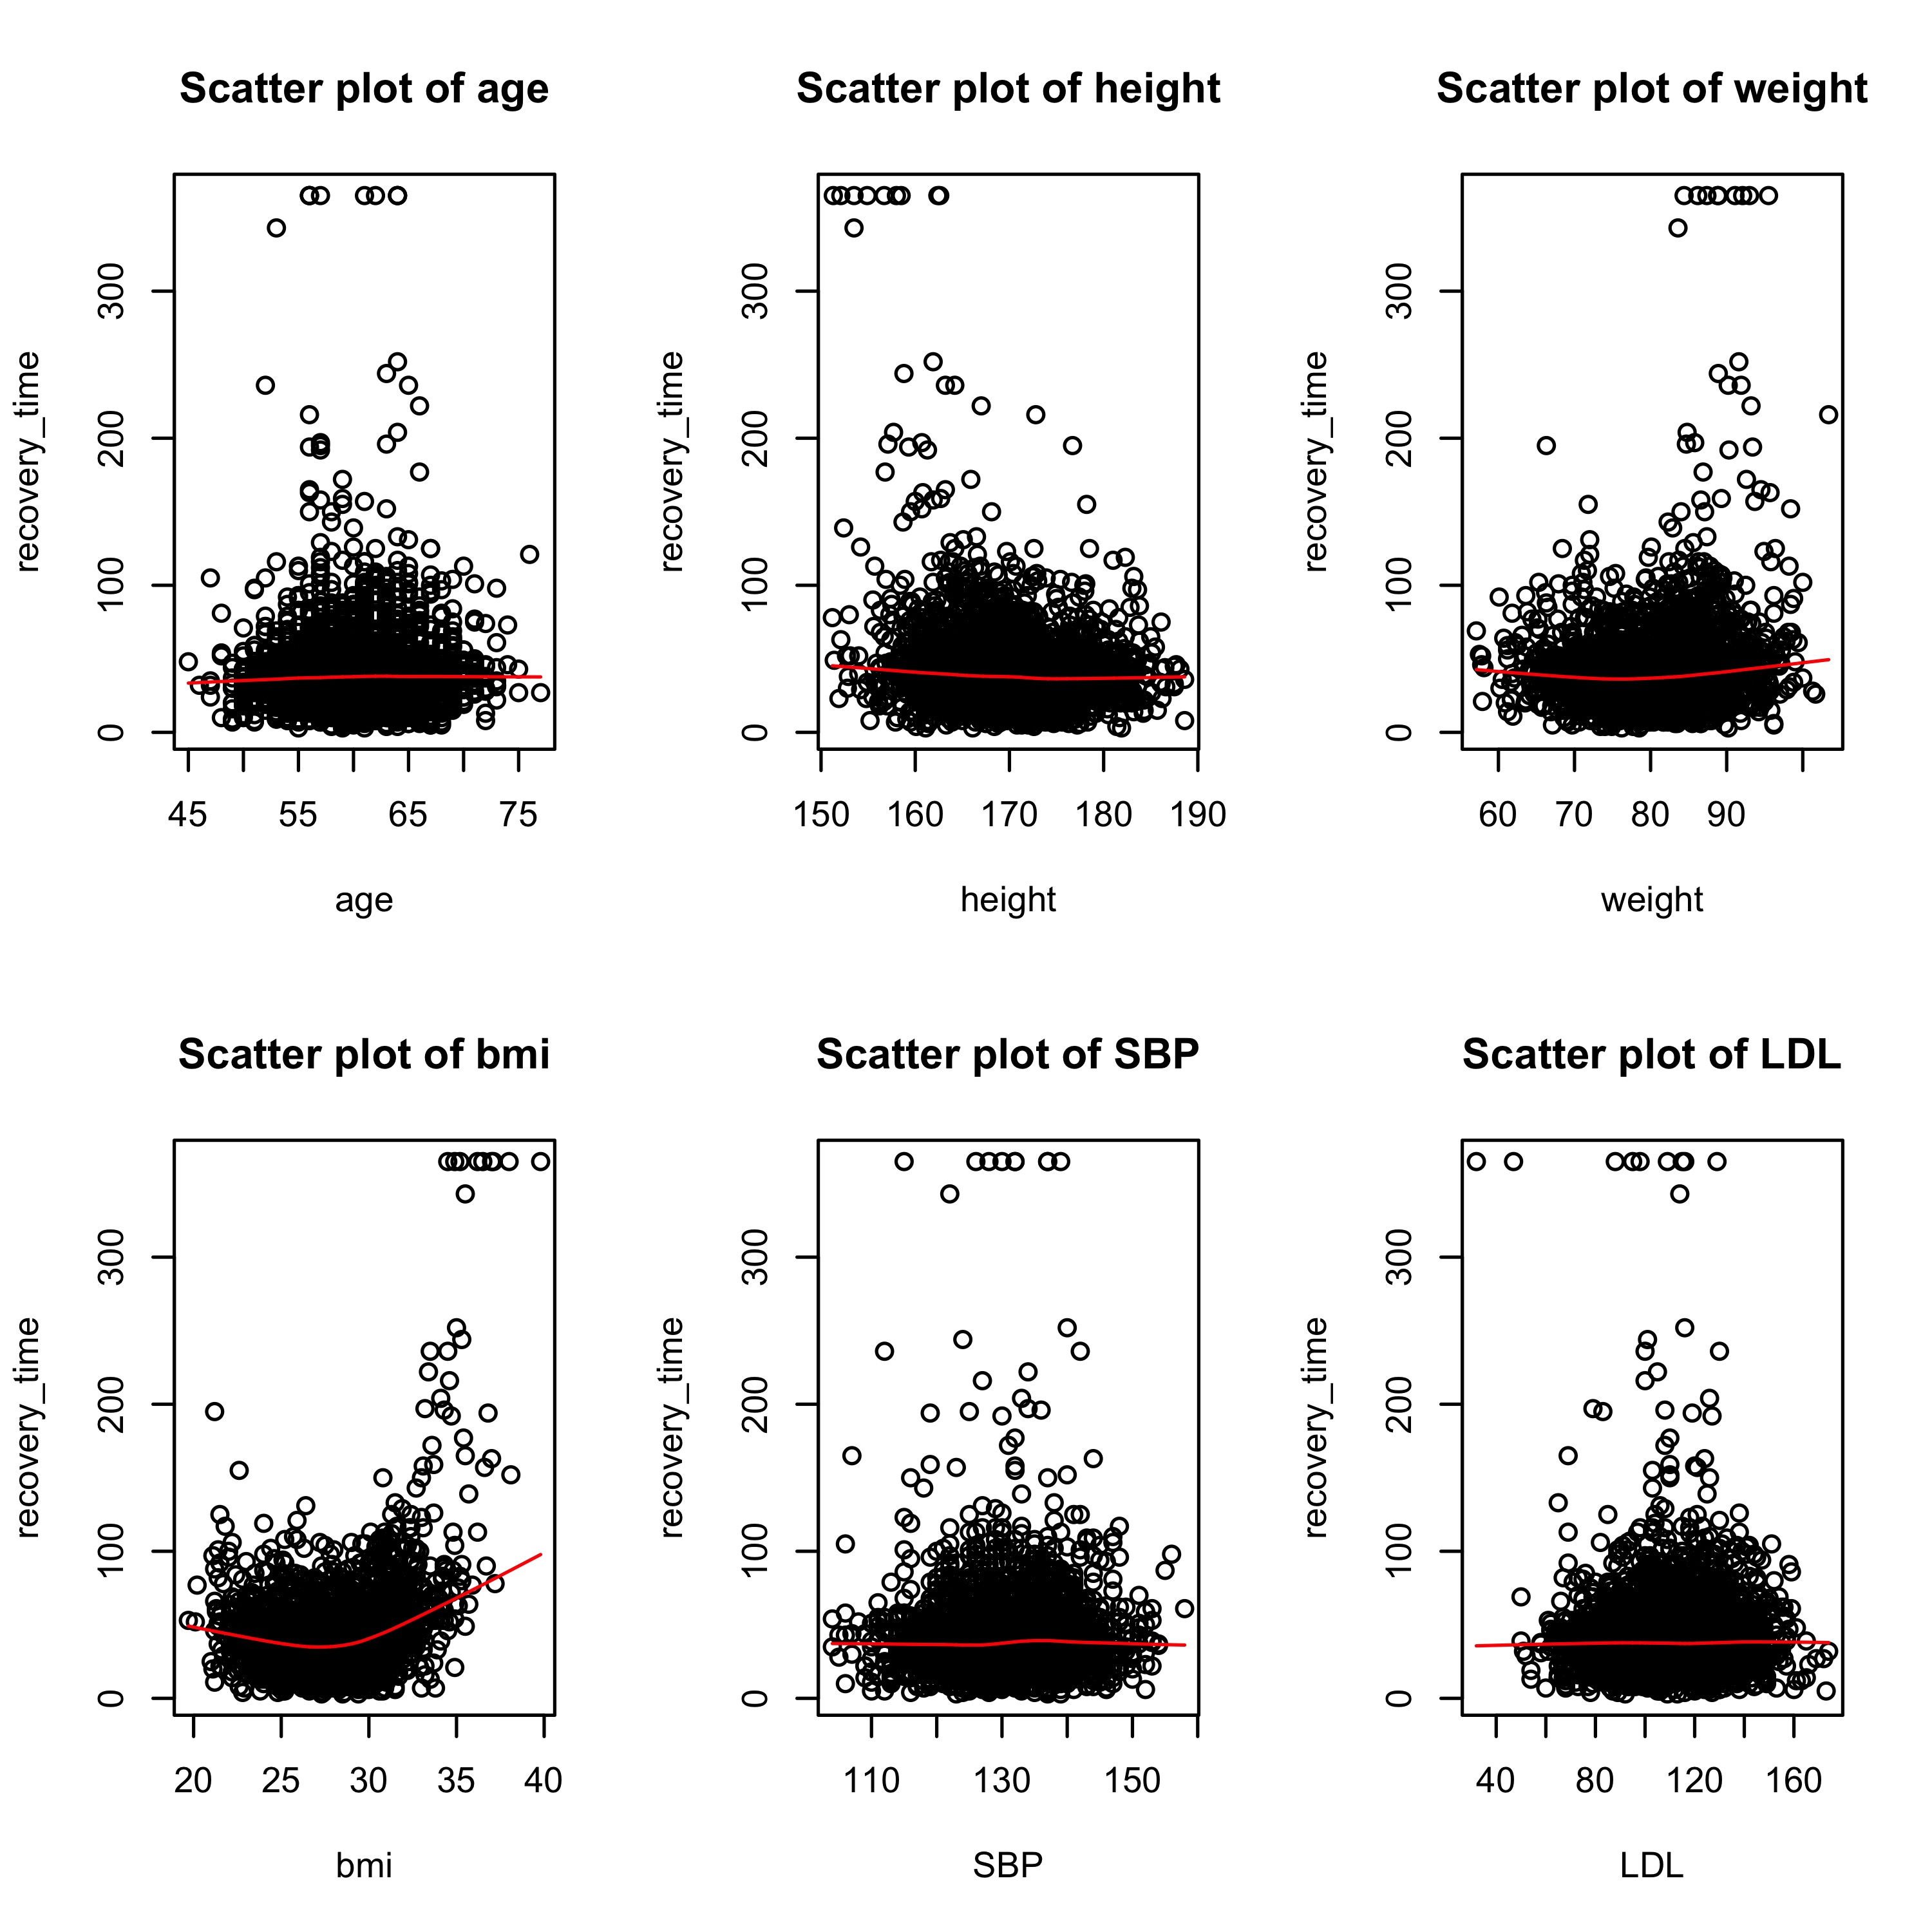
\includegraphics[width=0.36\textwidth]{eda/eda1_sactter.jpeg}\label{fig:eda1}}
    \hspace{0.1cm}
    % 2
    \subfigure[Boxplots of categorical variables]{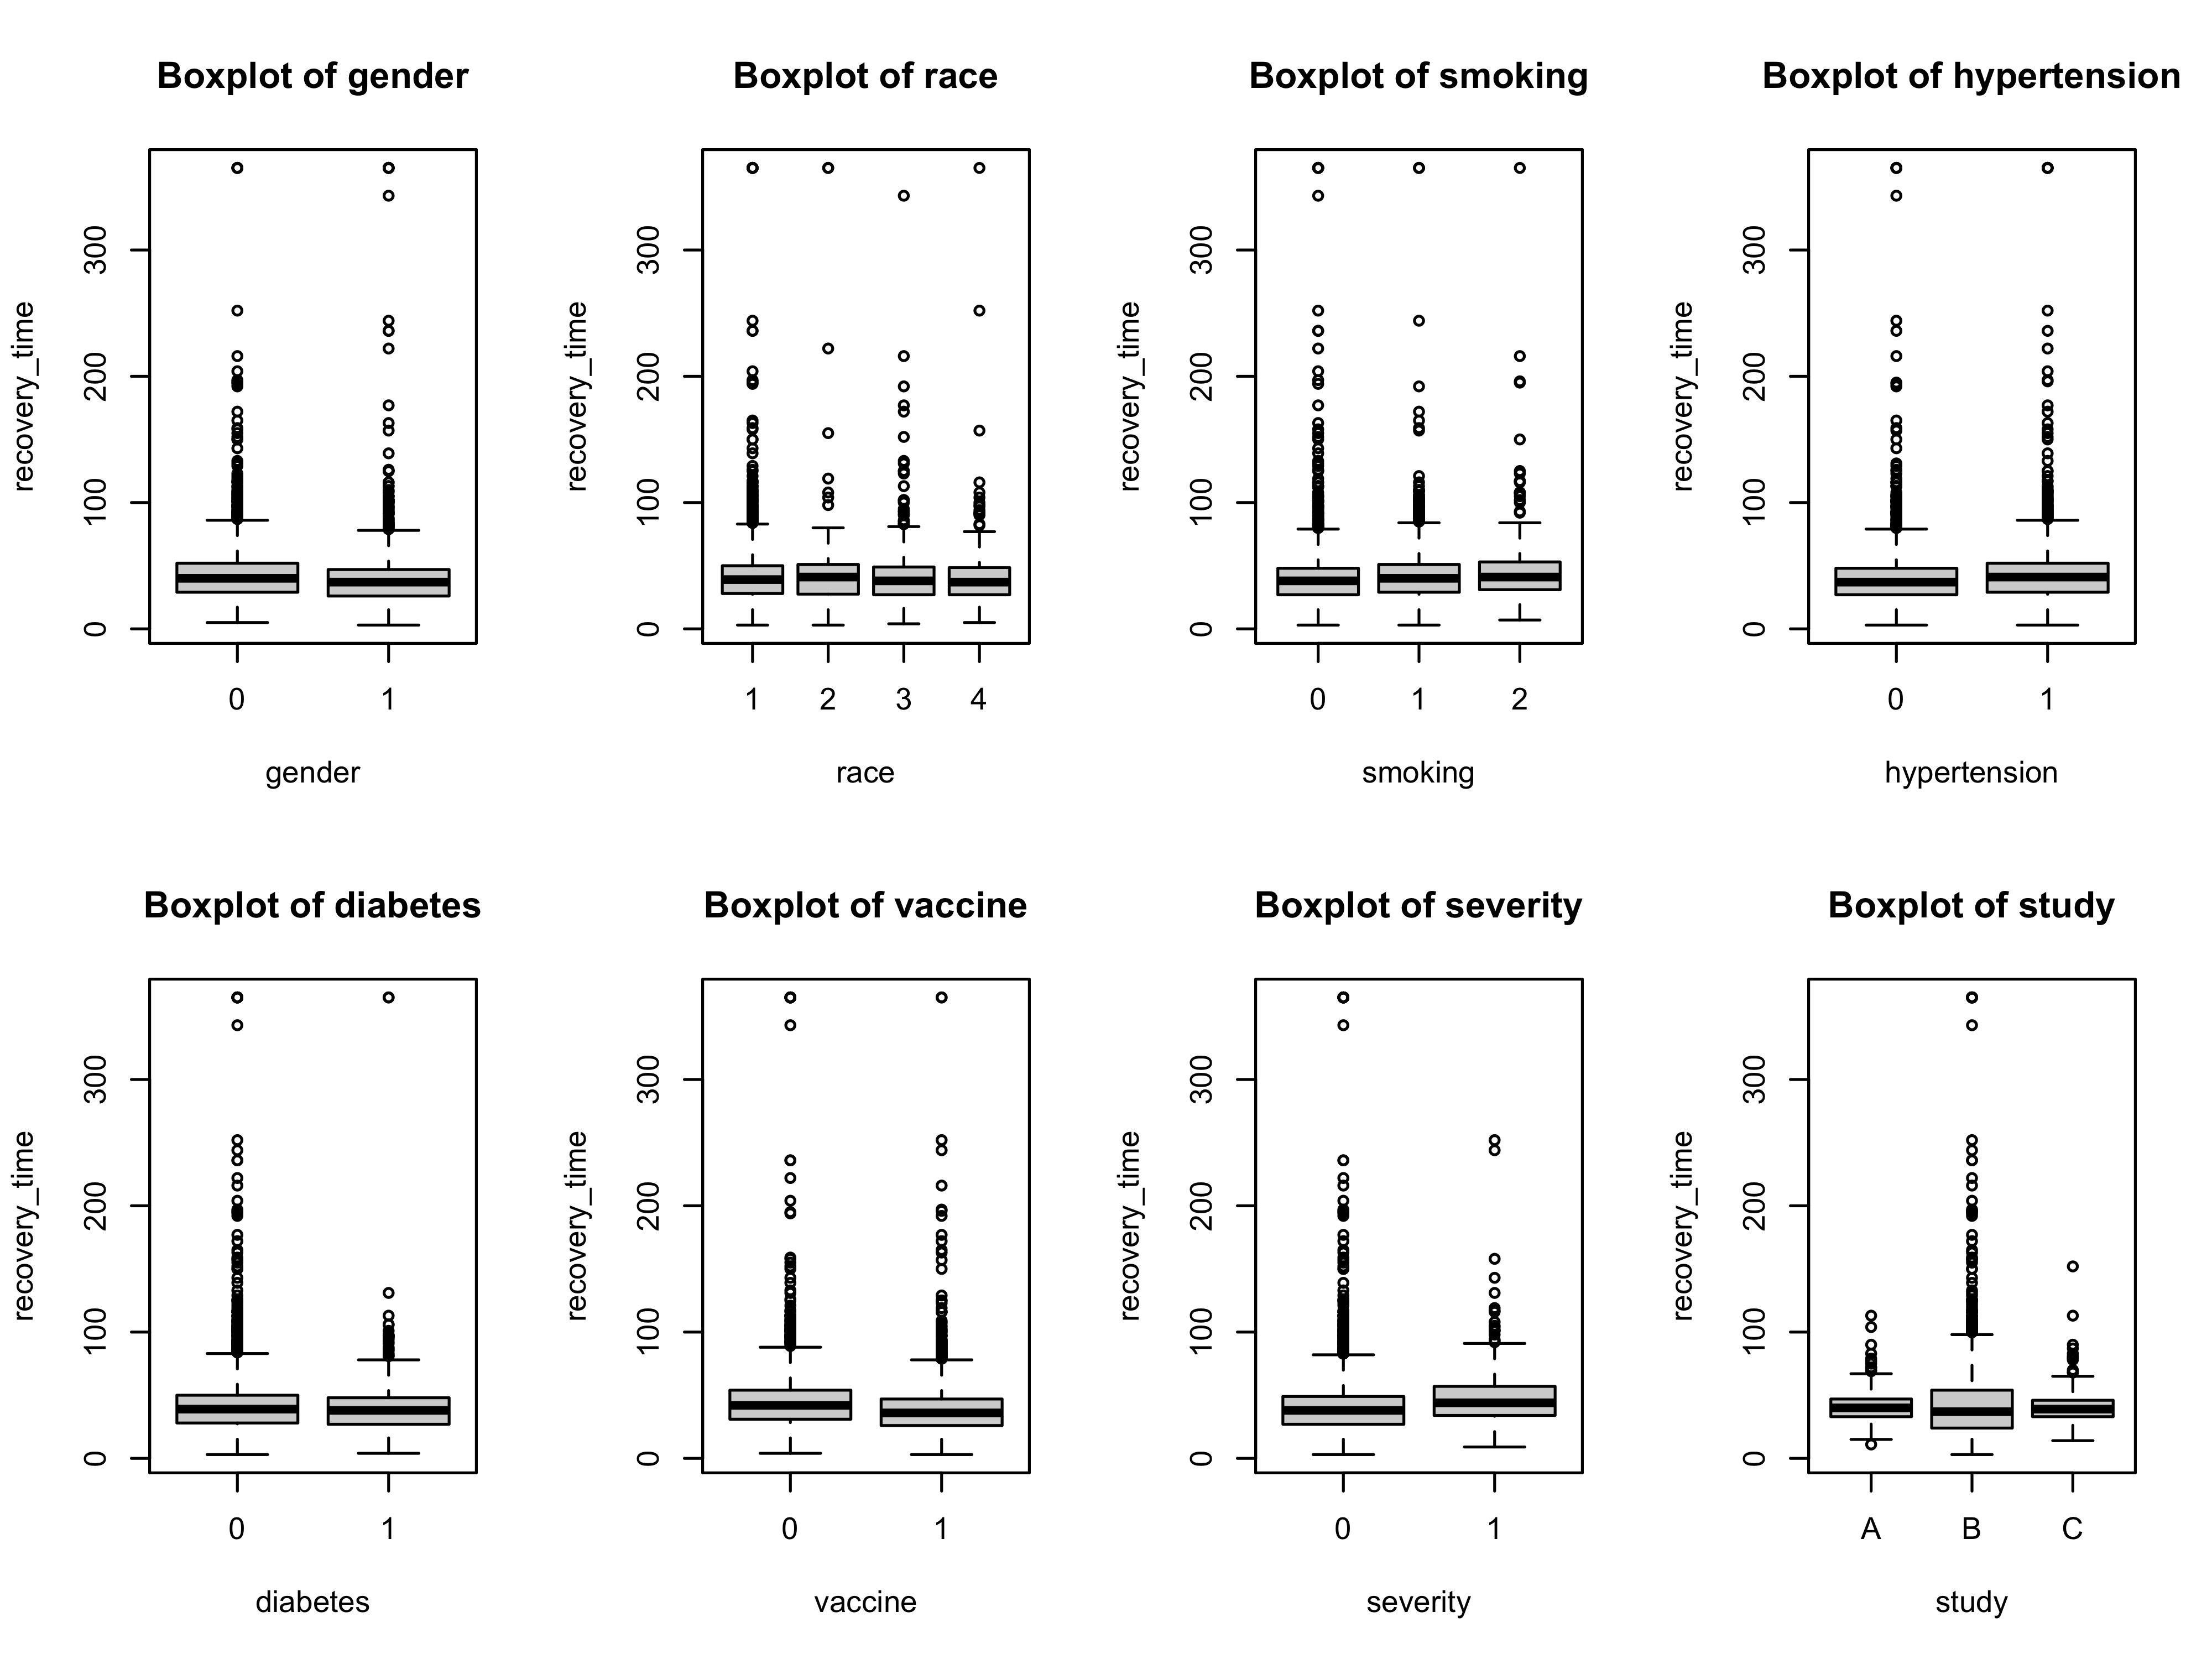
\includegraphics[width=0.48\textwidth]{eda/eda1_boxplot.jpeg}\label{fig:eda2}}
    
    % 3
    \subfigure[Boxplots of continuous variables]{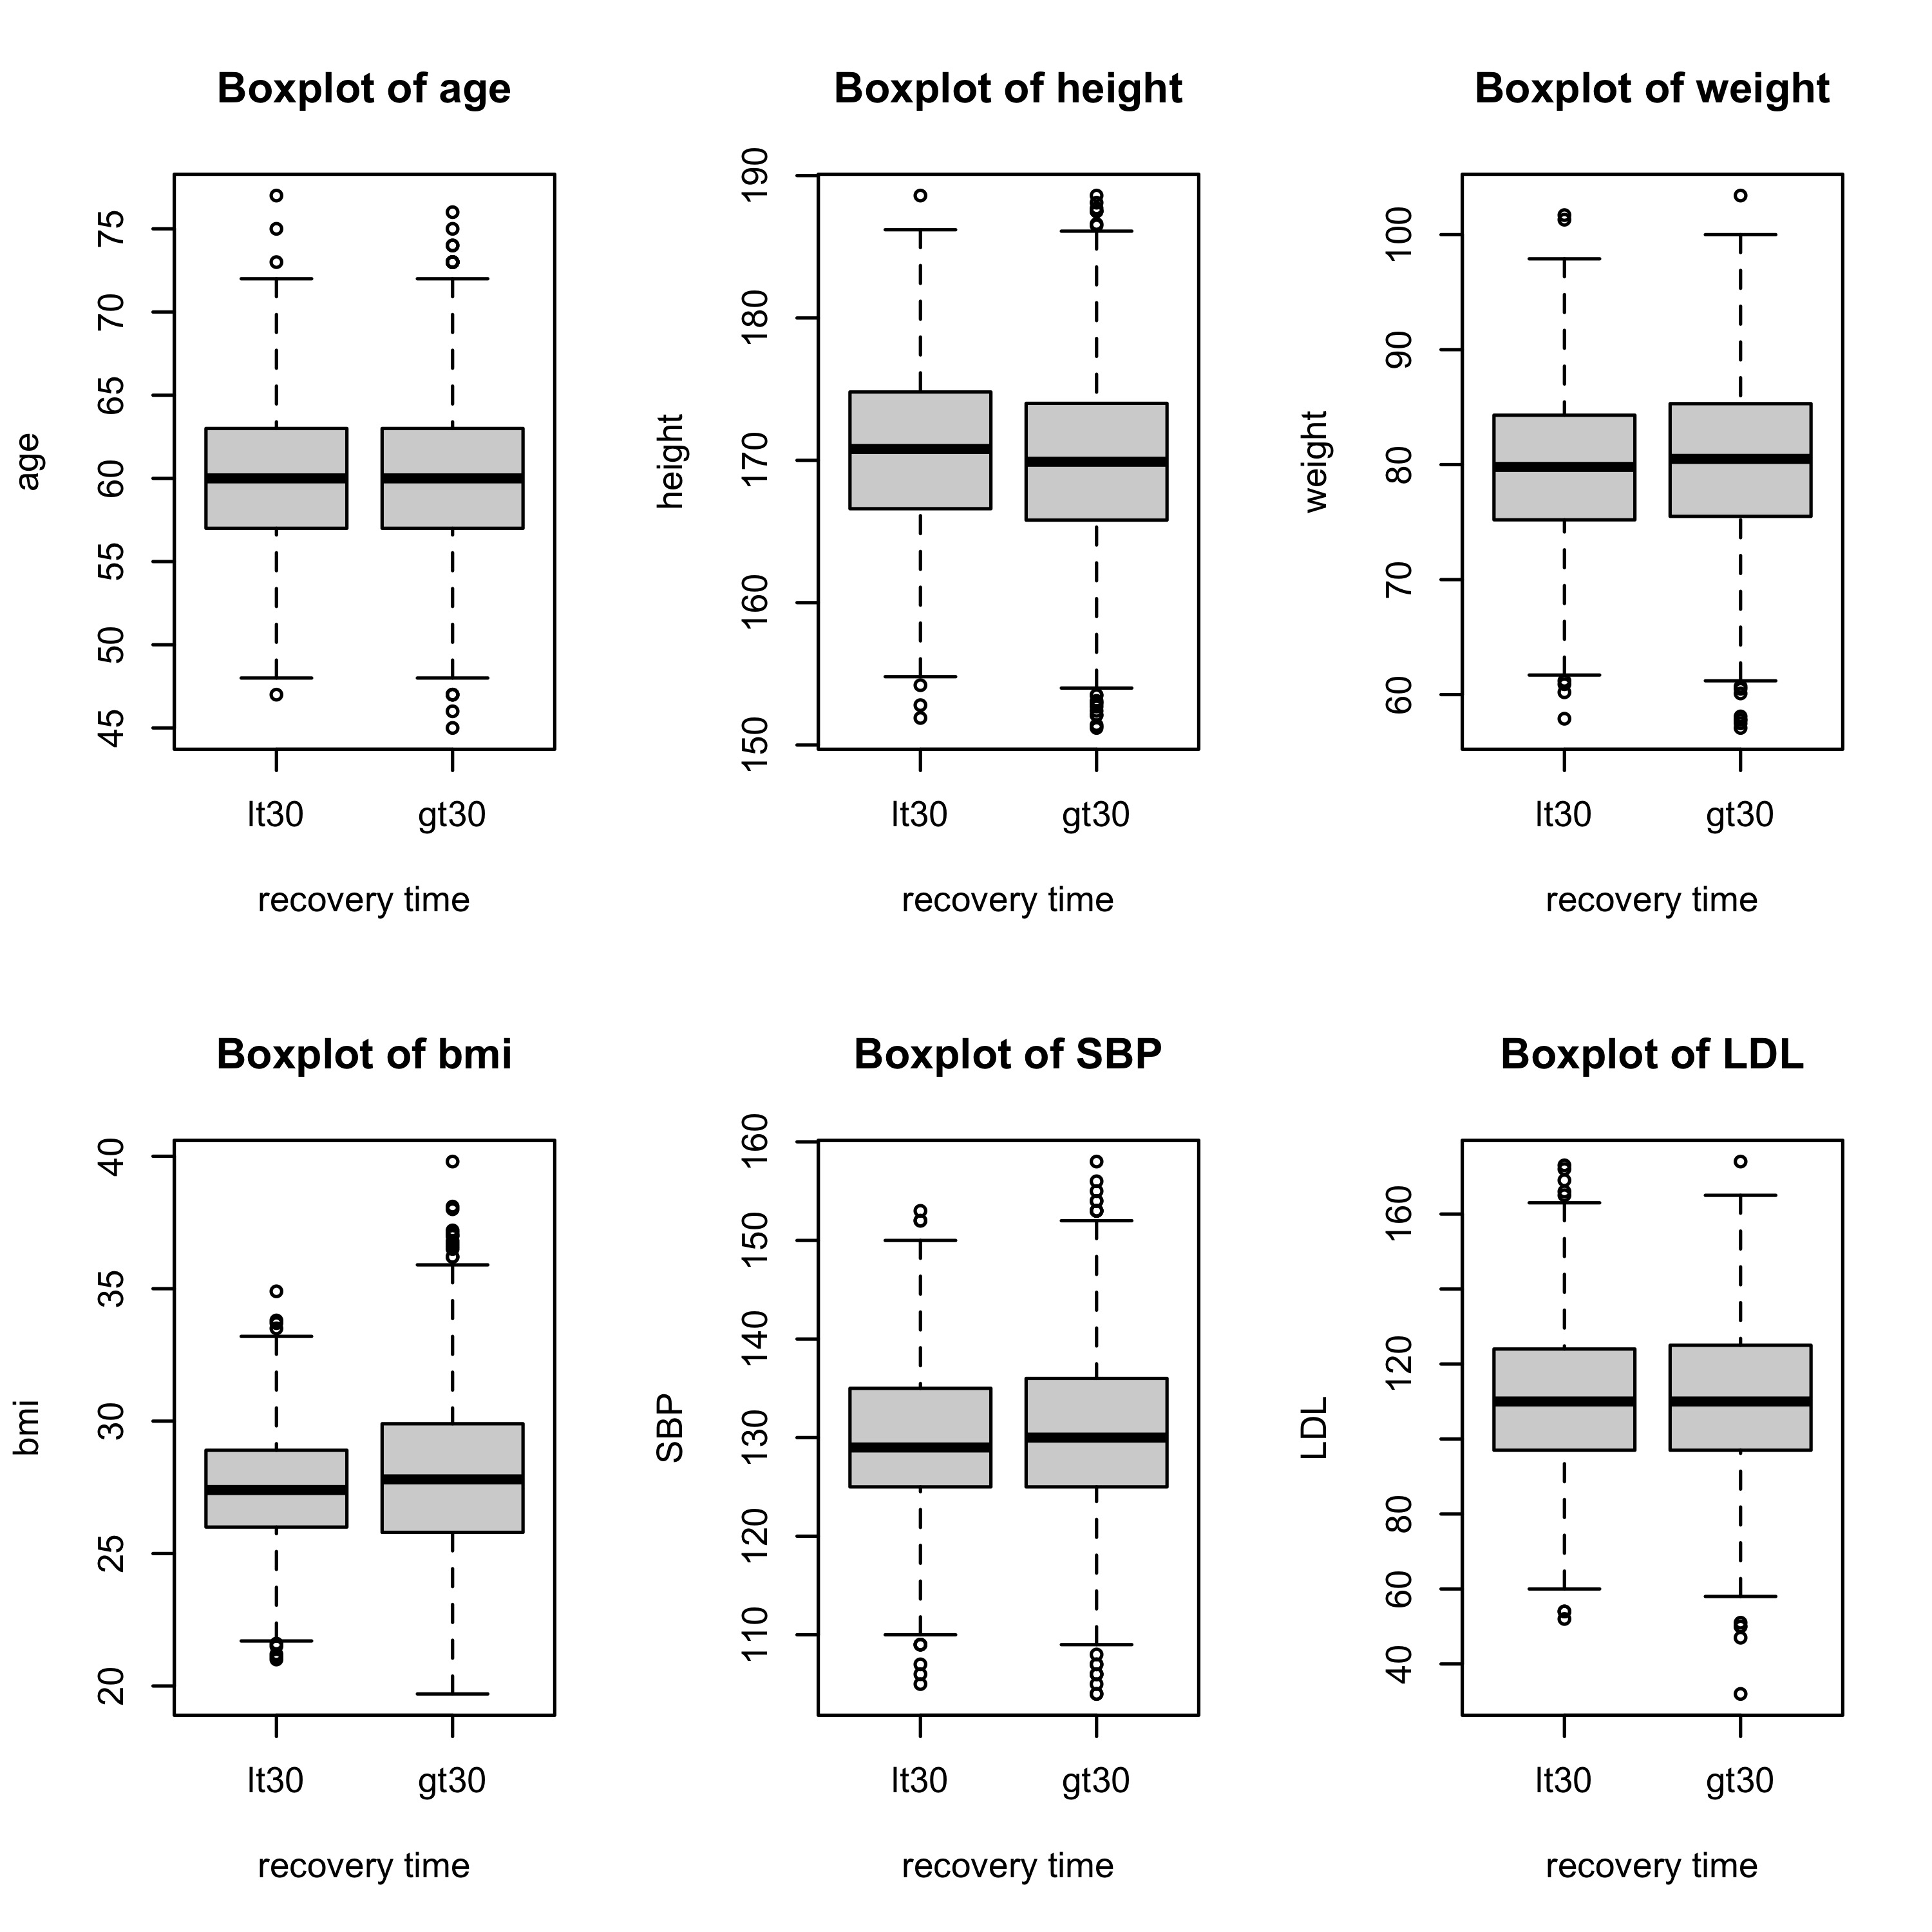
\includegraphics[width=0.36\textwidth]{eda/eda2_boxplot.jpeg}\label{fig:eda3}}
    \hspace{0.1cm}
    % 4
    \subfigure[Barplots of categorical variables]{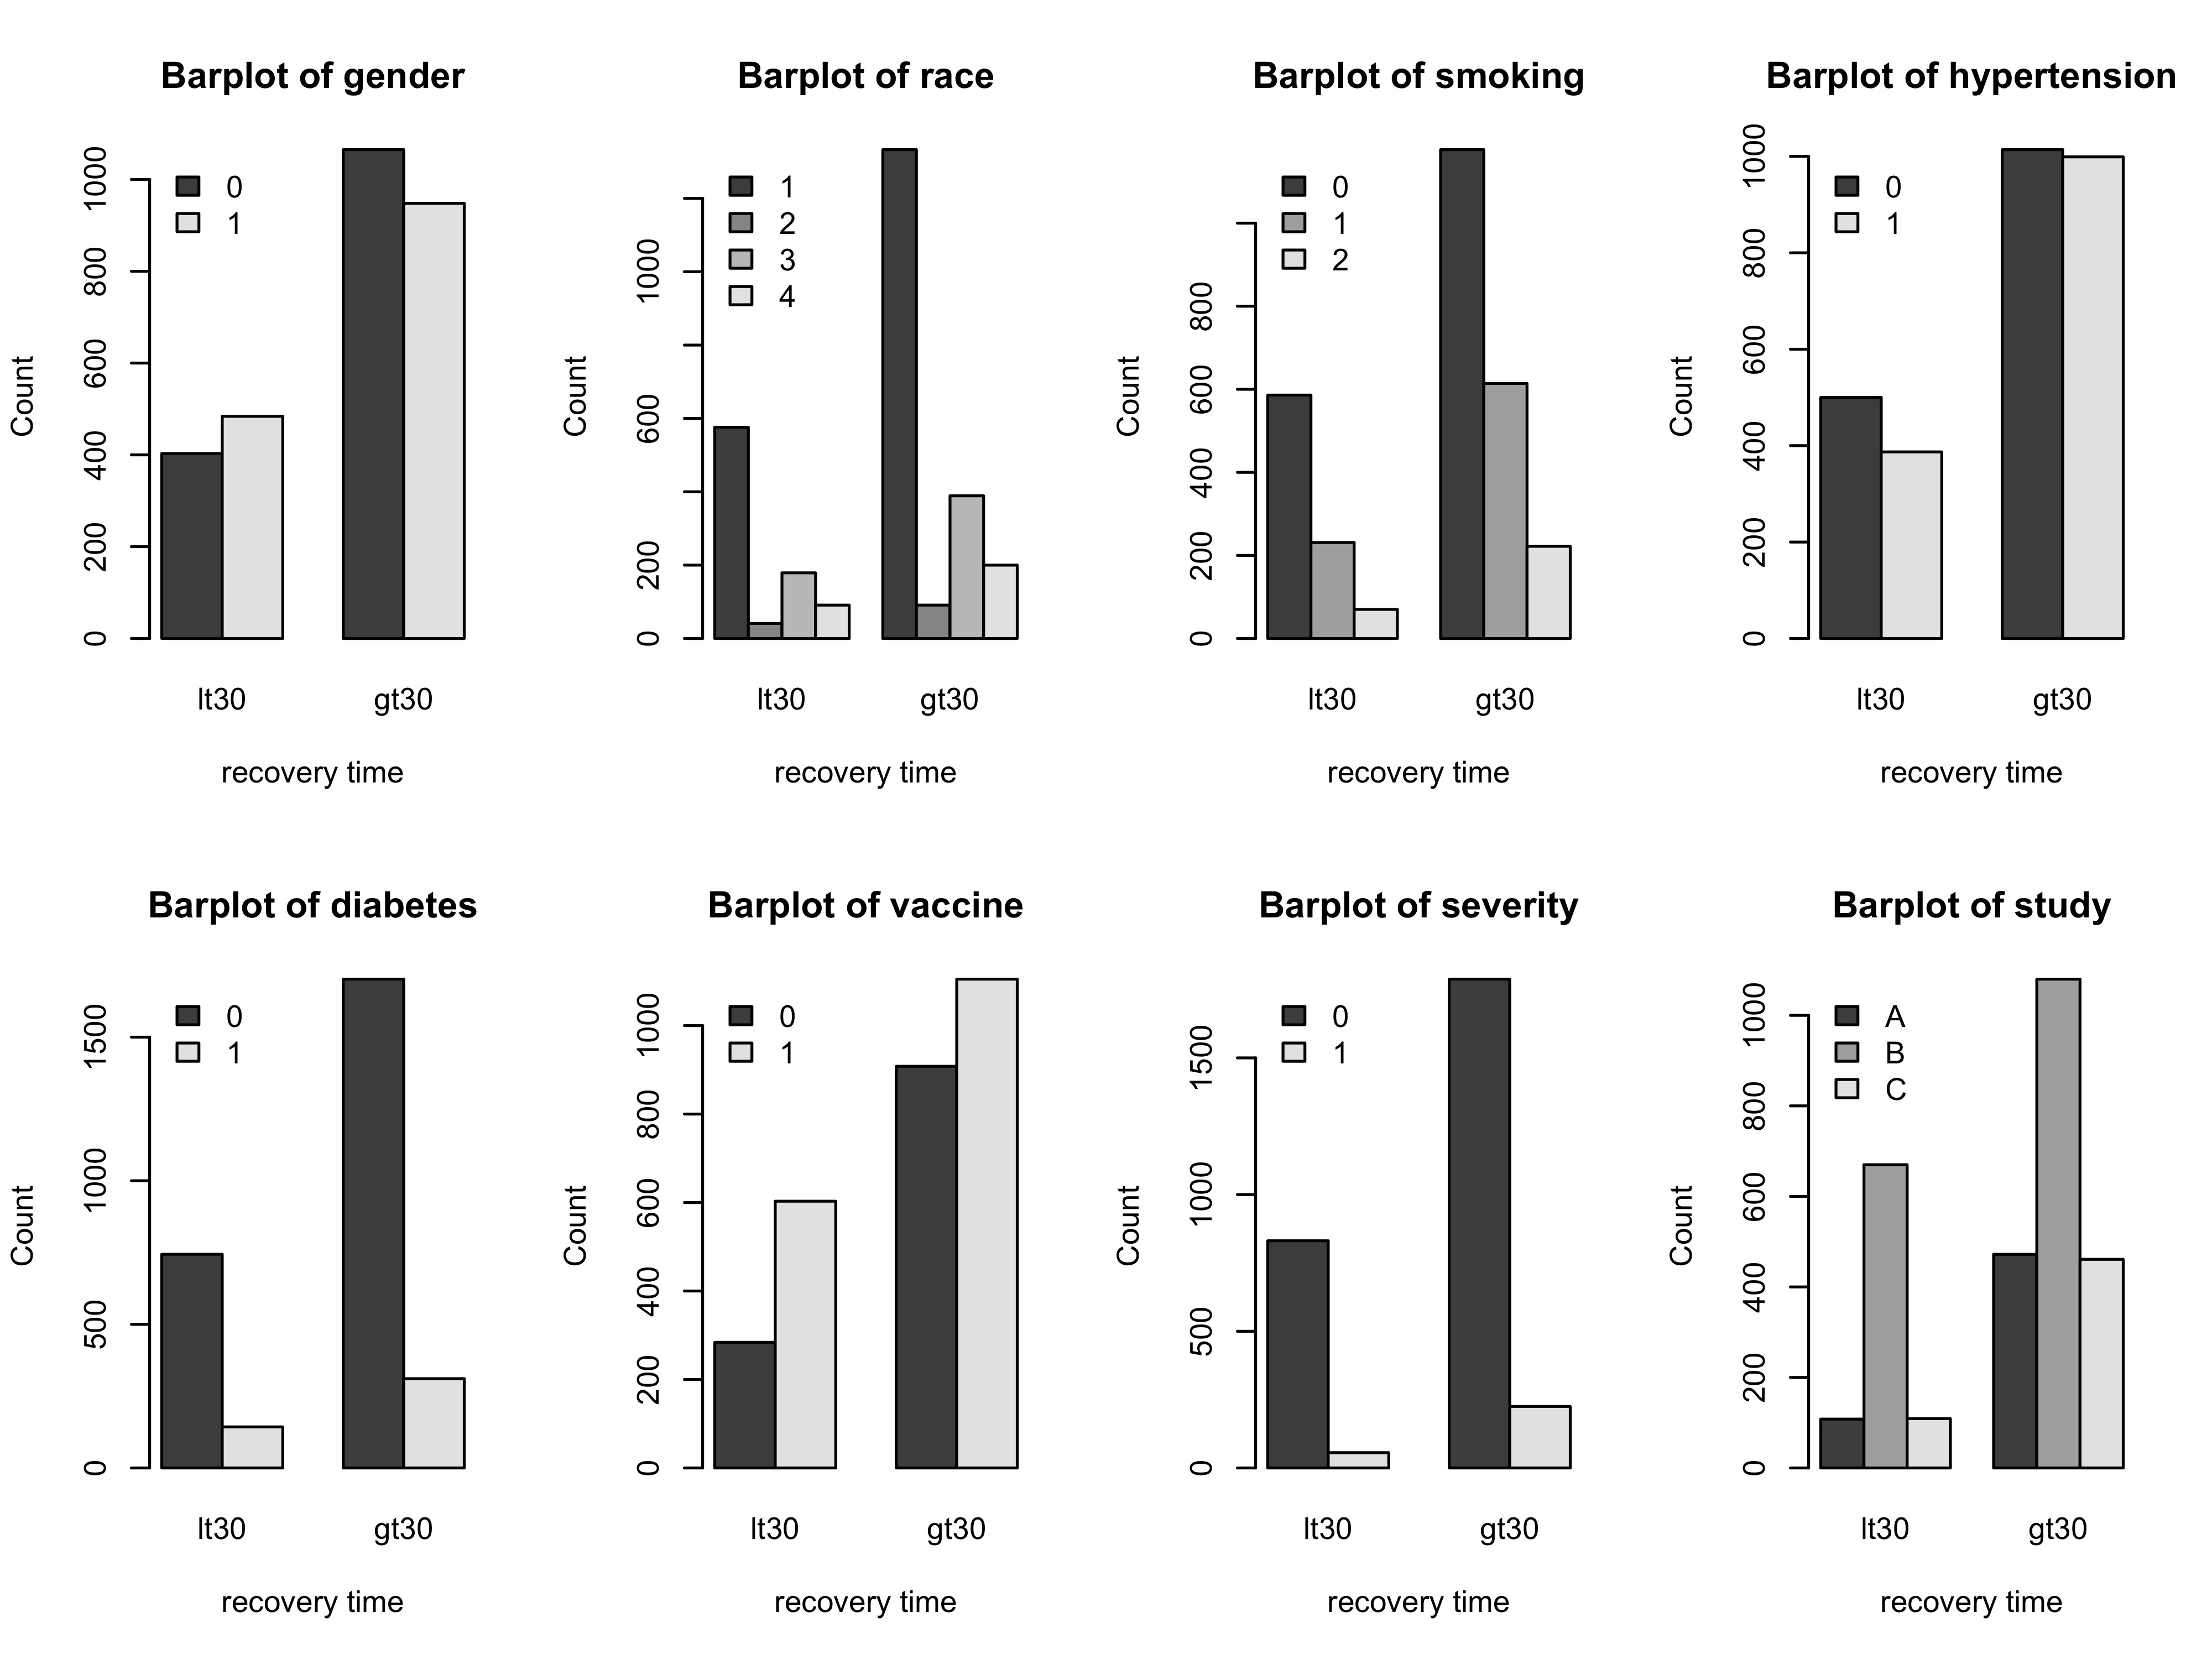
\includegraphics[width=0.48\textwidth]{eda/eda2_barplot.jpeg}\label{fig:eda4}}
    
    % 5
    \subfigure[Histogram of continuous response]{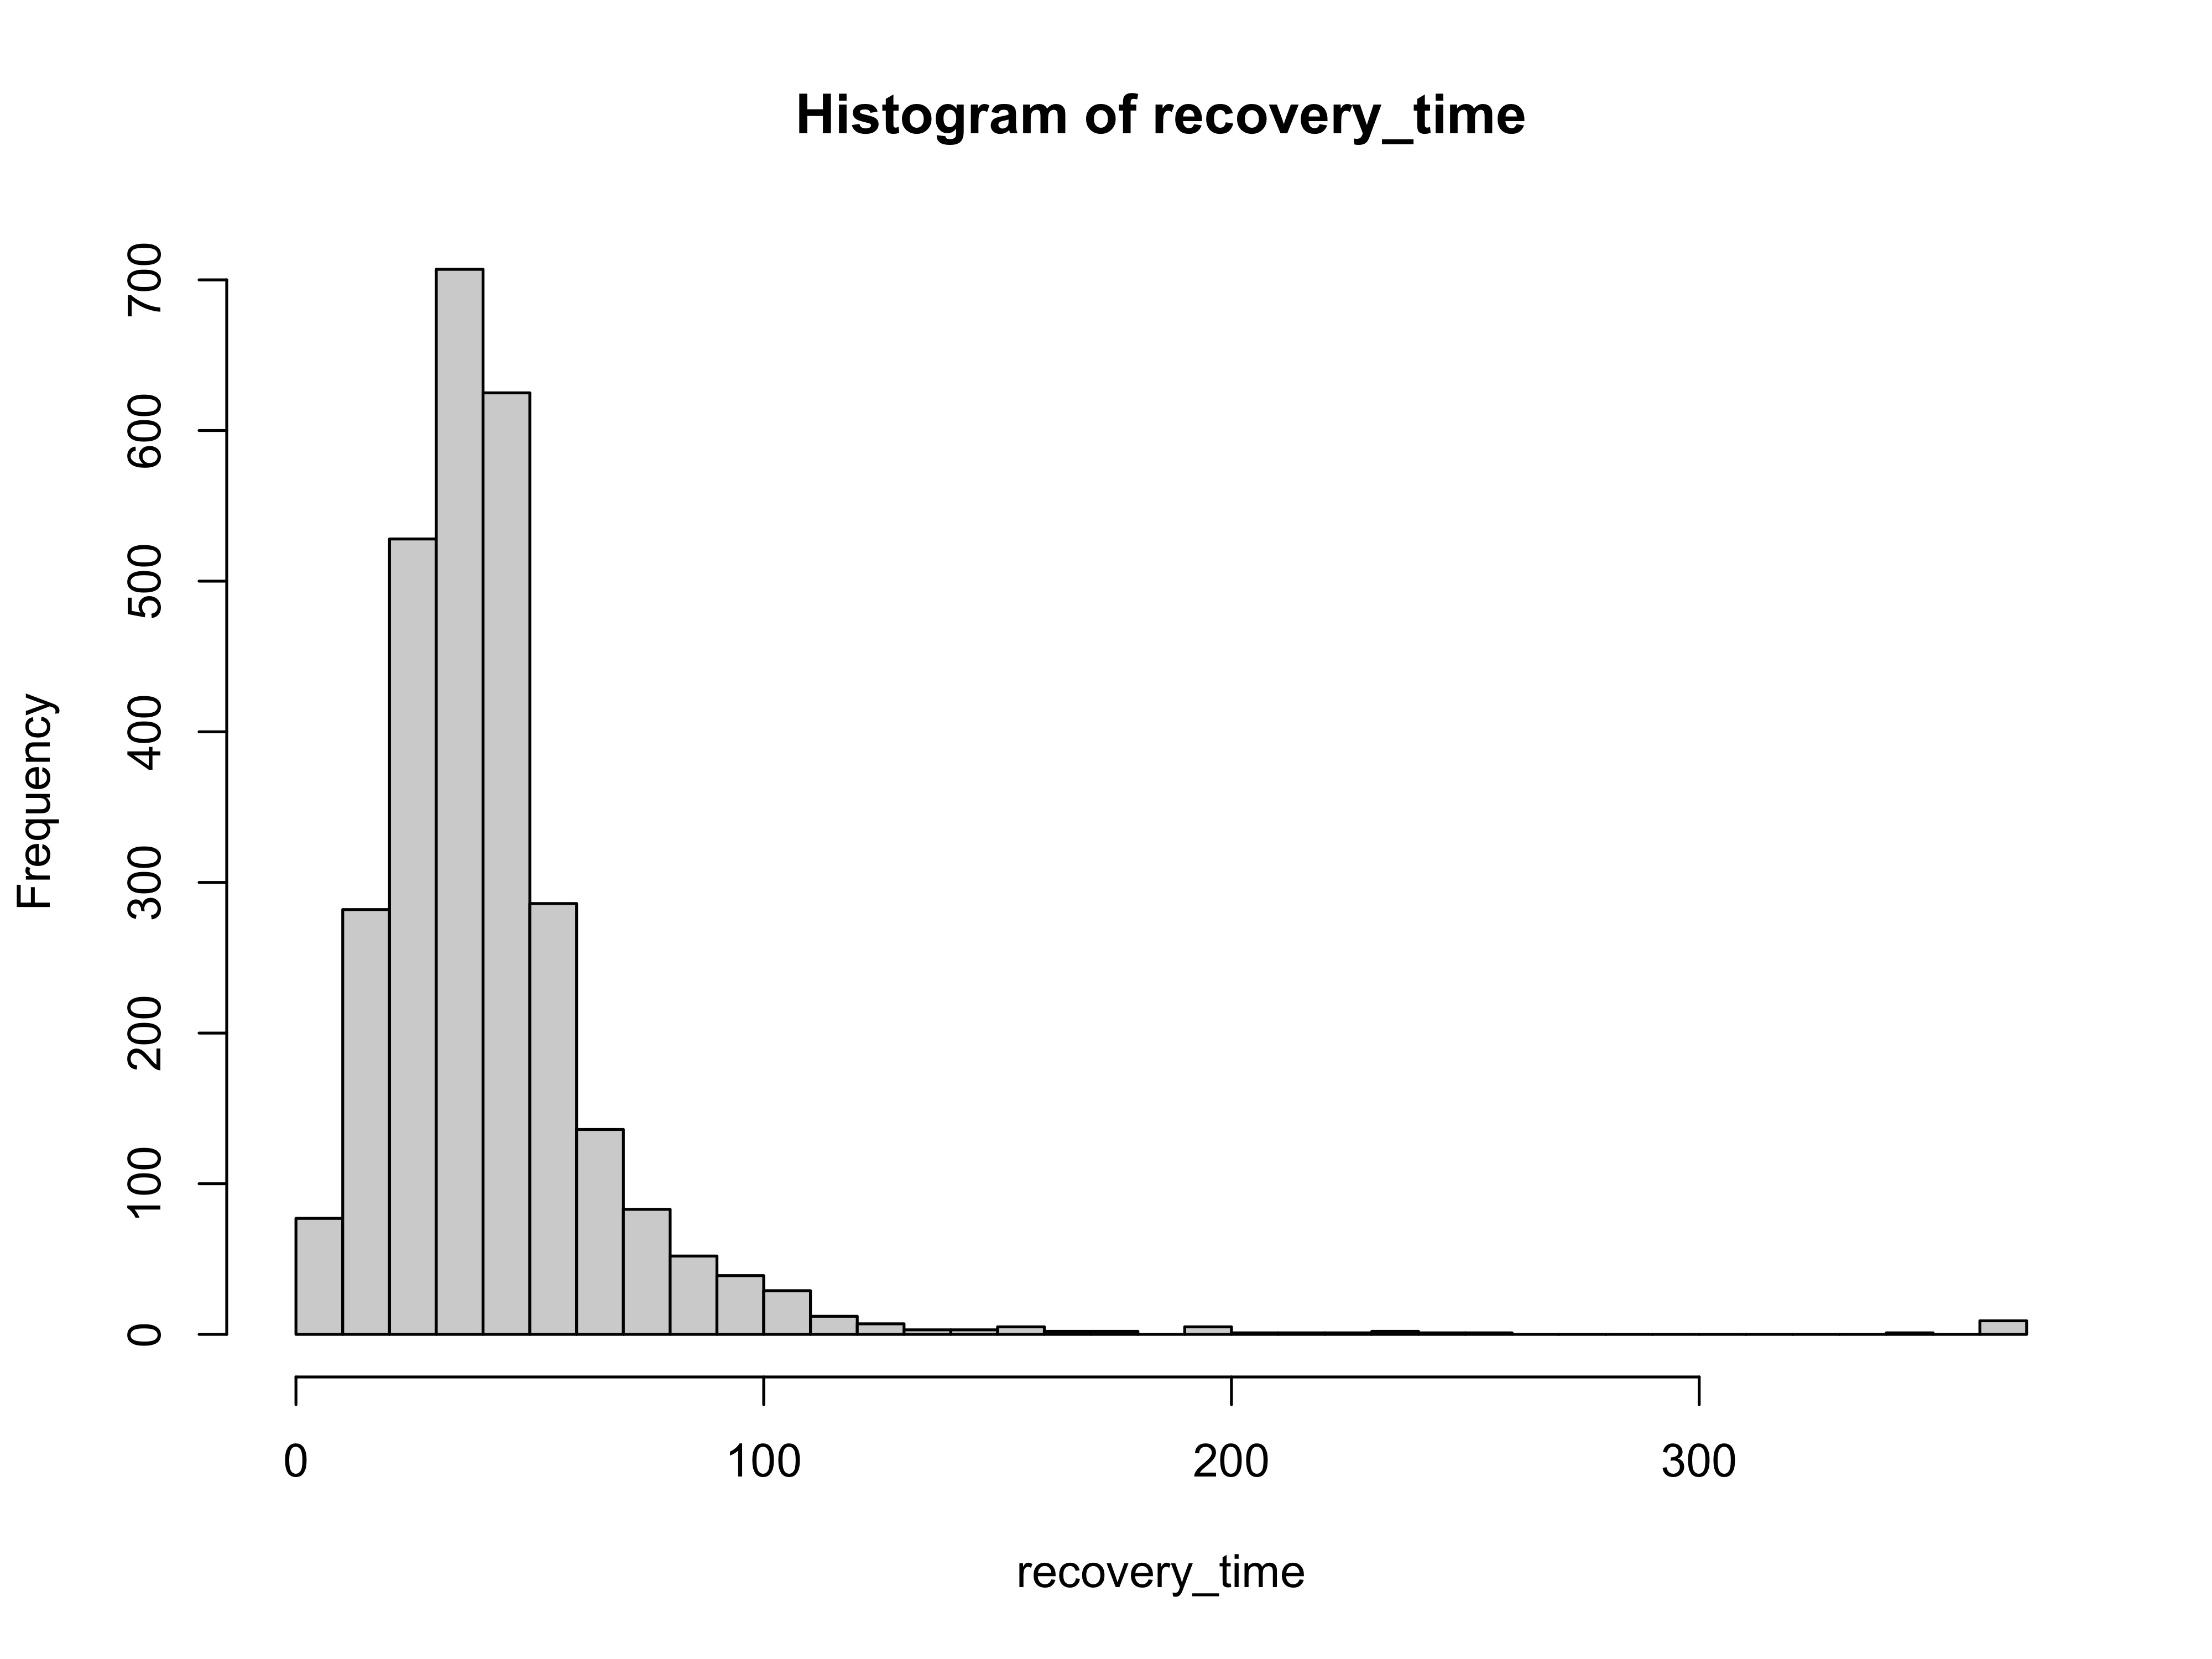
\includegraphics[width=0.4\textwidth]{eda/eda1_res_hist.jpeg}\label{fig:eda5}}
    \hspace{0.1cm}
    % 6
    \subfigure[Barplot of binary response]{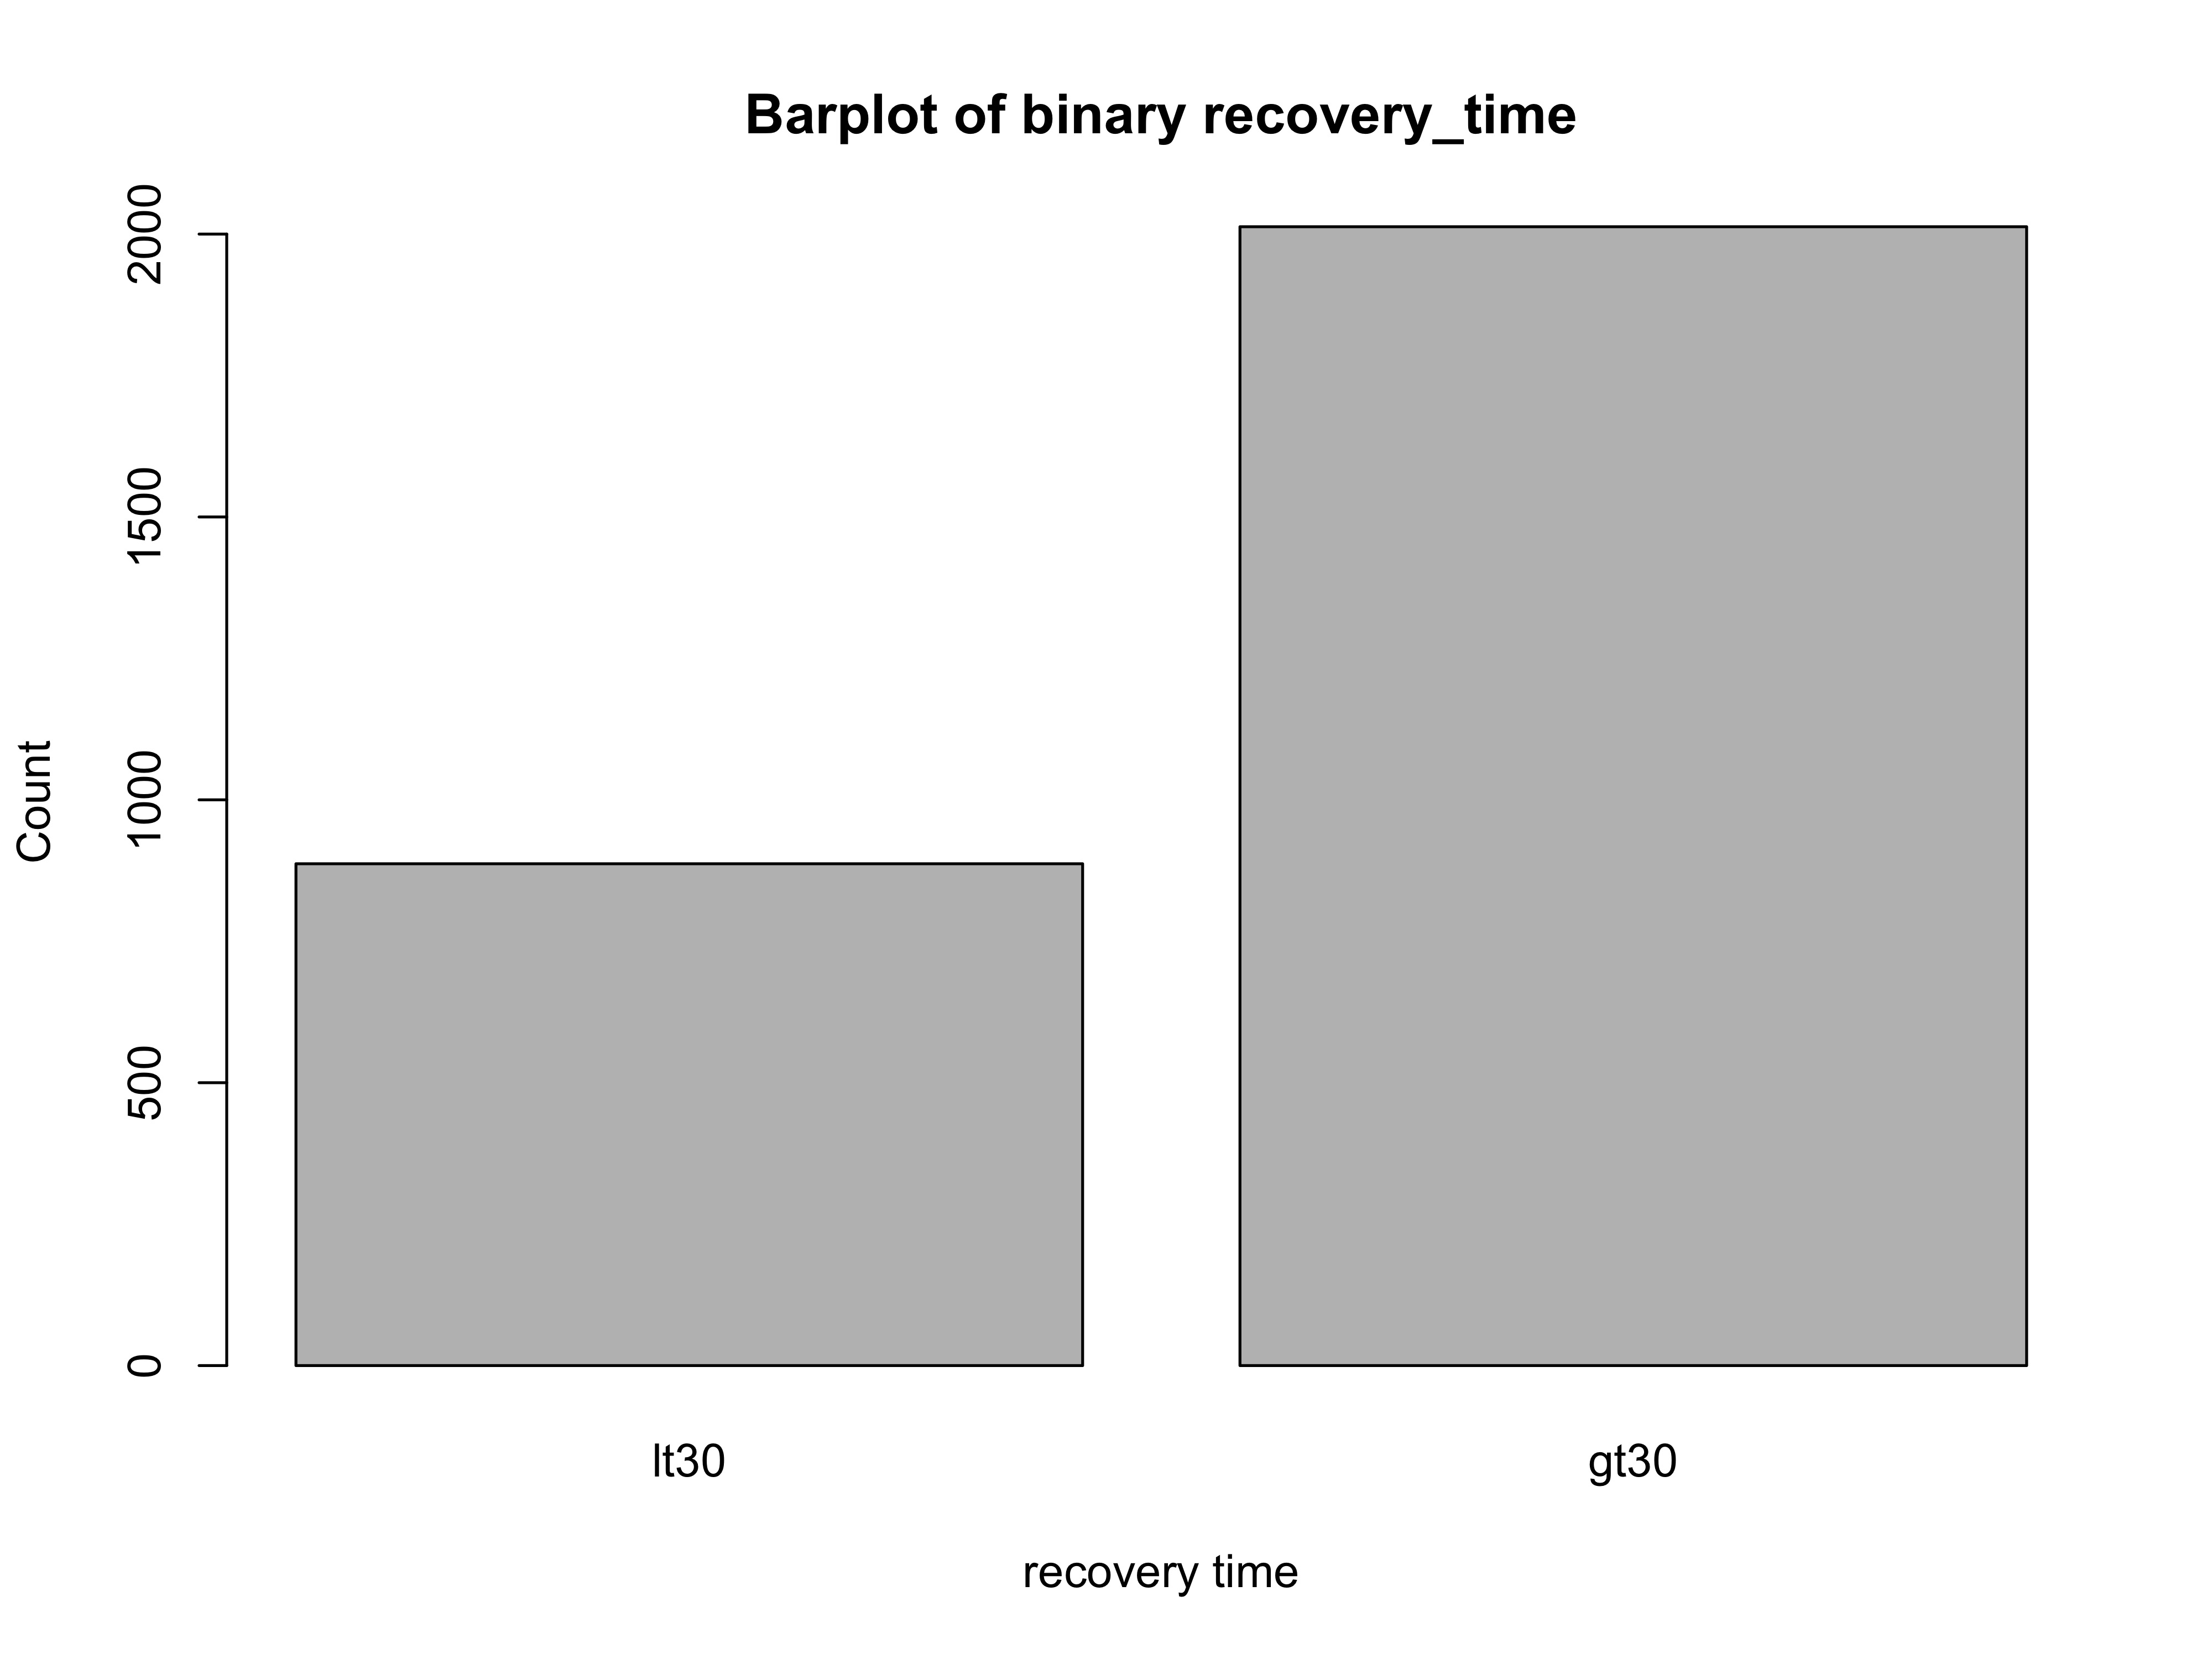
\includegraphics[width=0.4\textwidth]{eda/eda2_res_barplot.jpeg}\label{fig:eda6}}

    % 7
    \subfigure[Correlation plot of continuous variables]{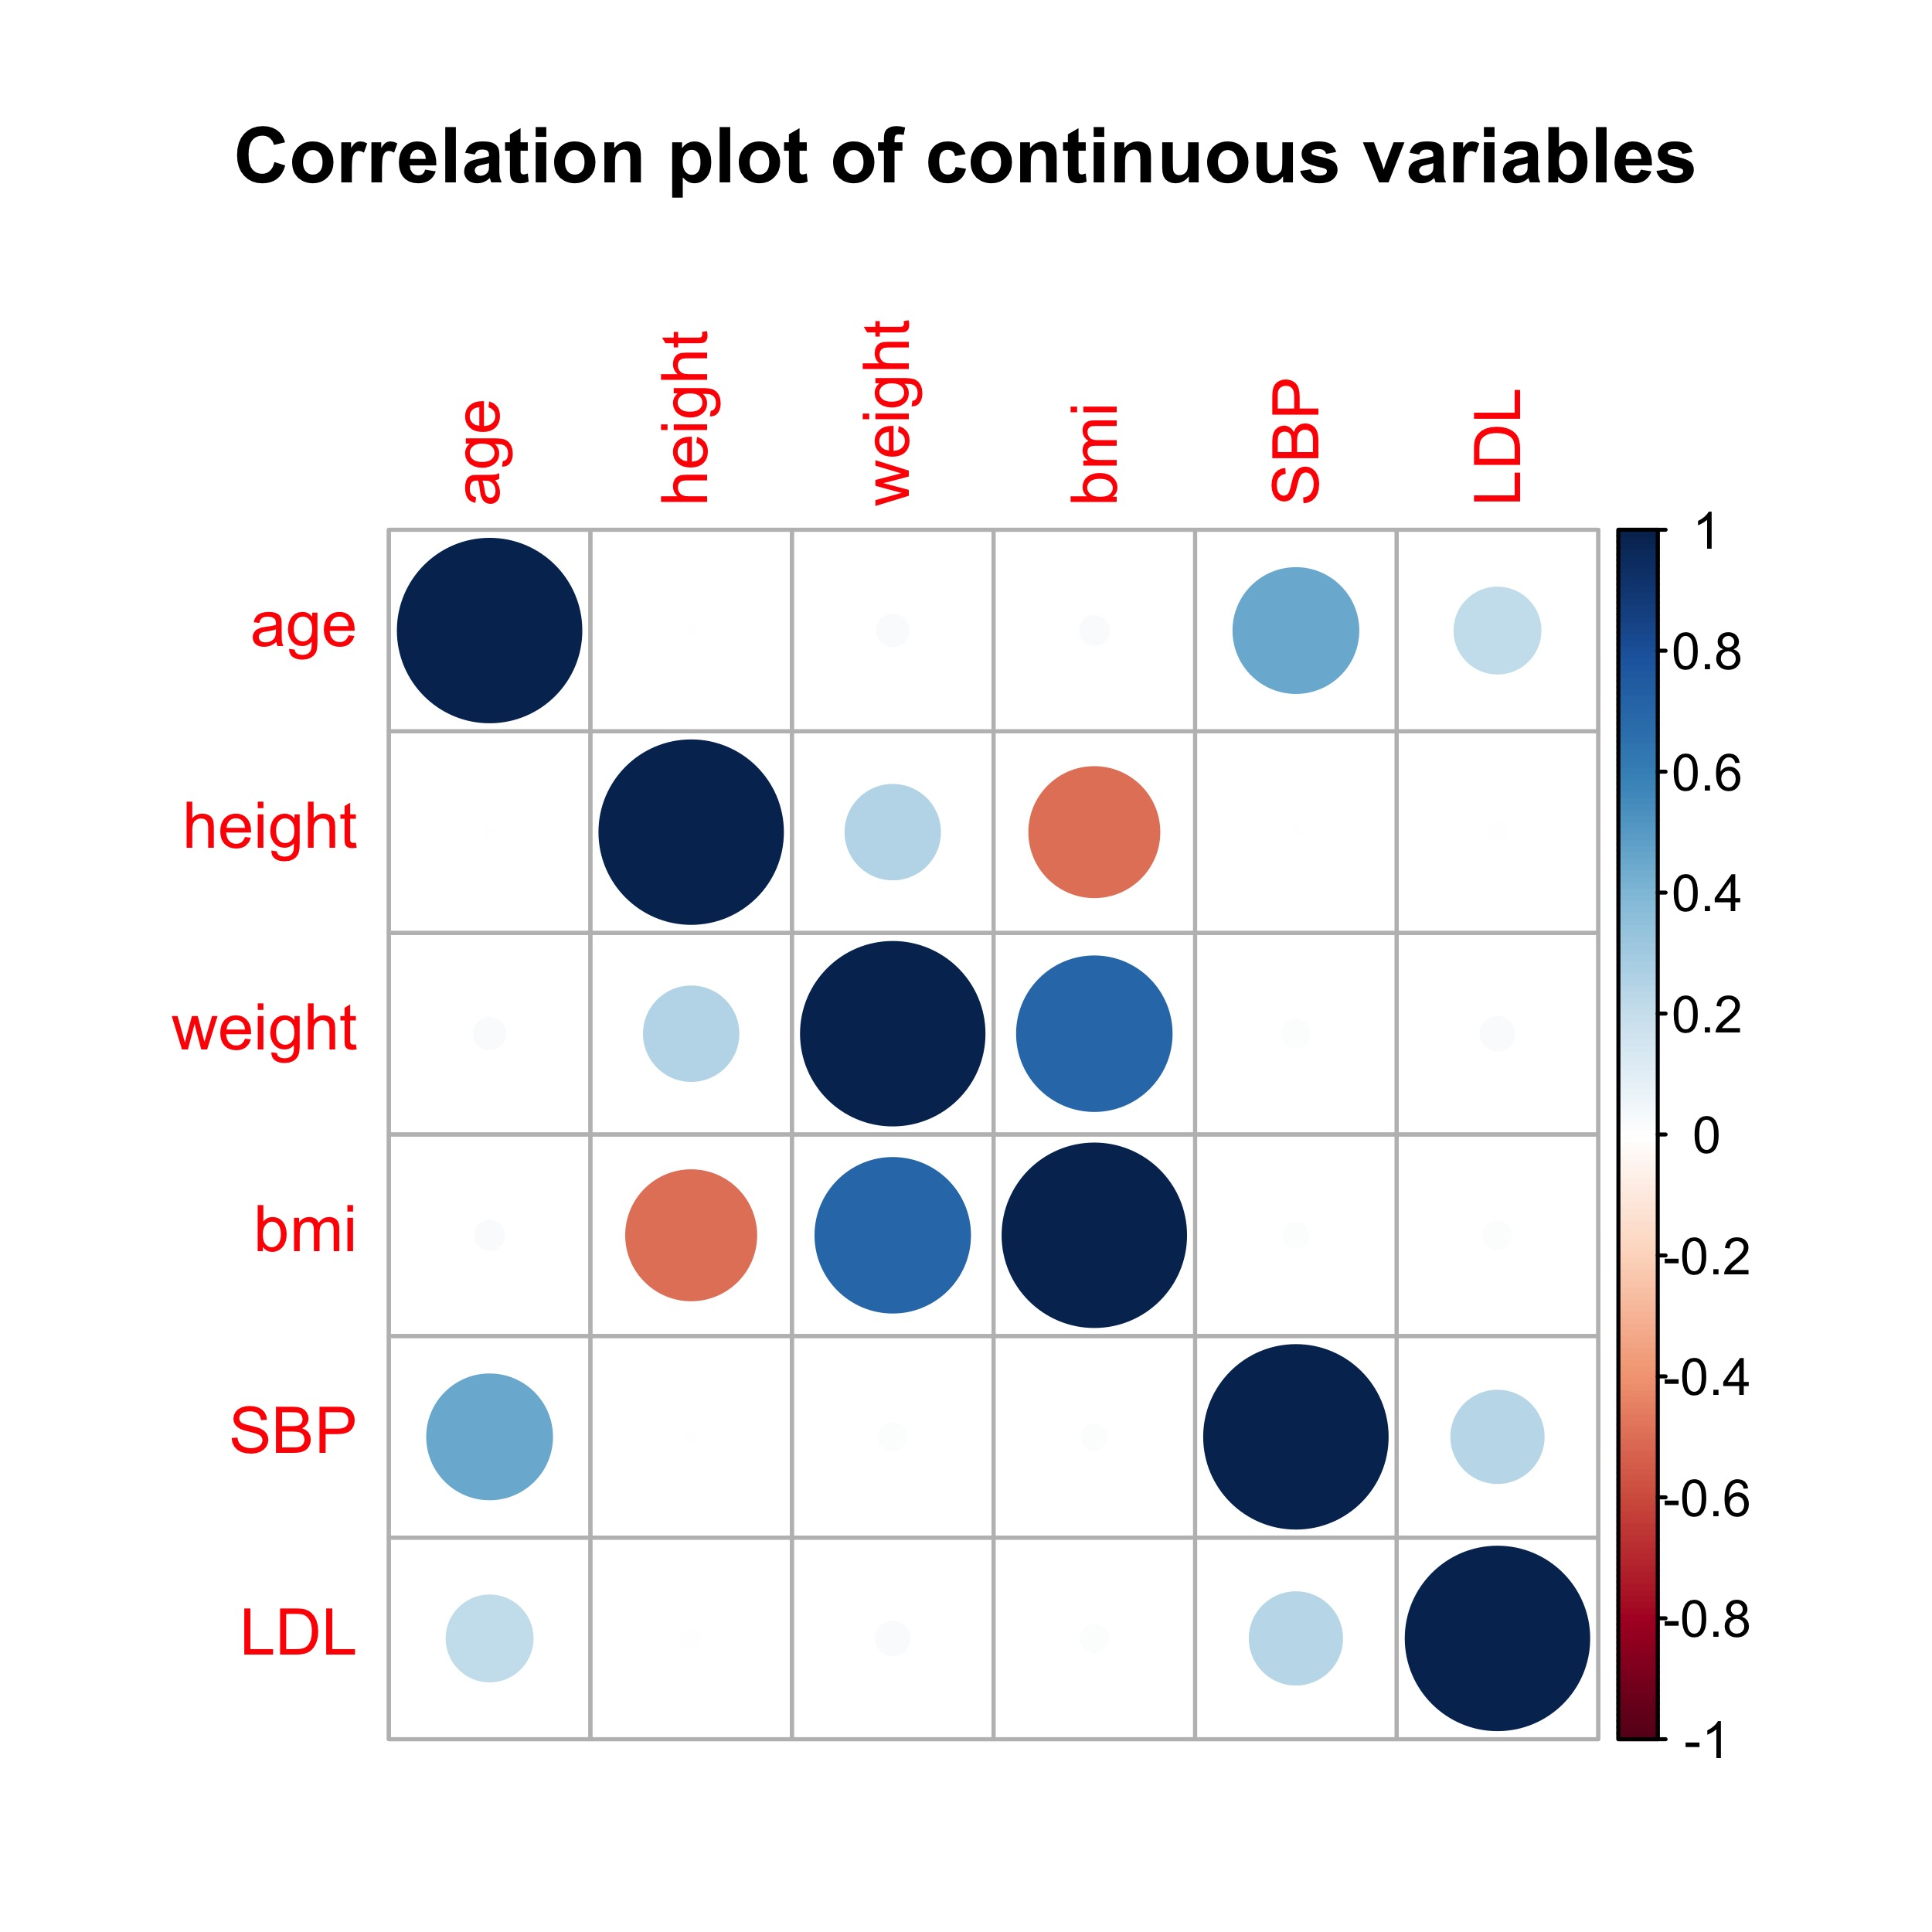
\includegraphics[width=0.4\textwidth]{eda/eda1_corr.jpeg}\label{fig:eda7}}
    
    \caption{EDA plots}
    \label{fig:eda}
\end{figure}


\begin{figure}
    \centering
    
    % 1
    \subfigure[LASSO]{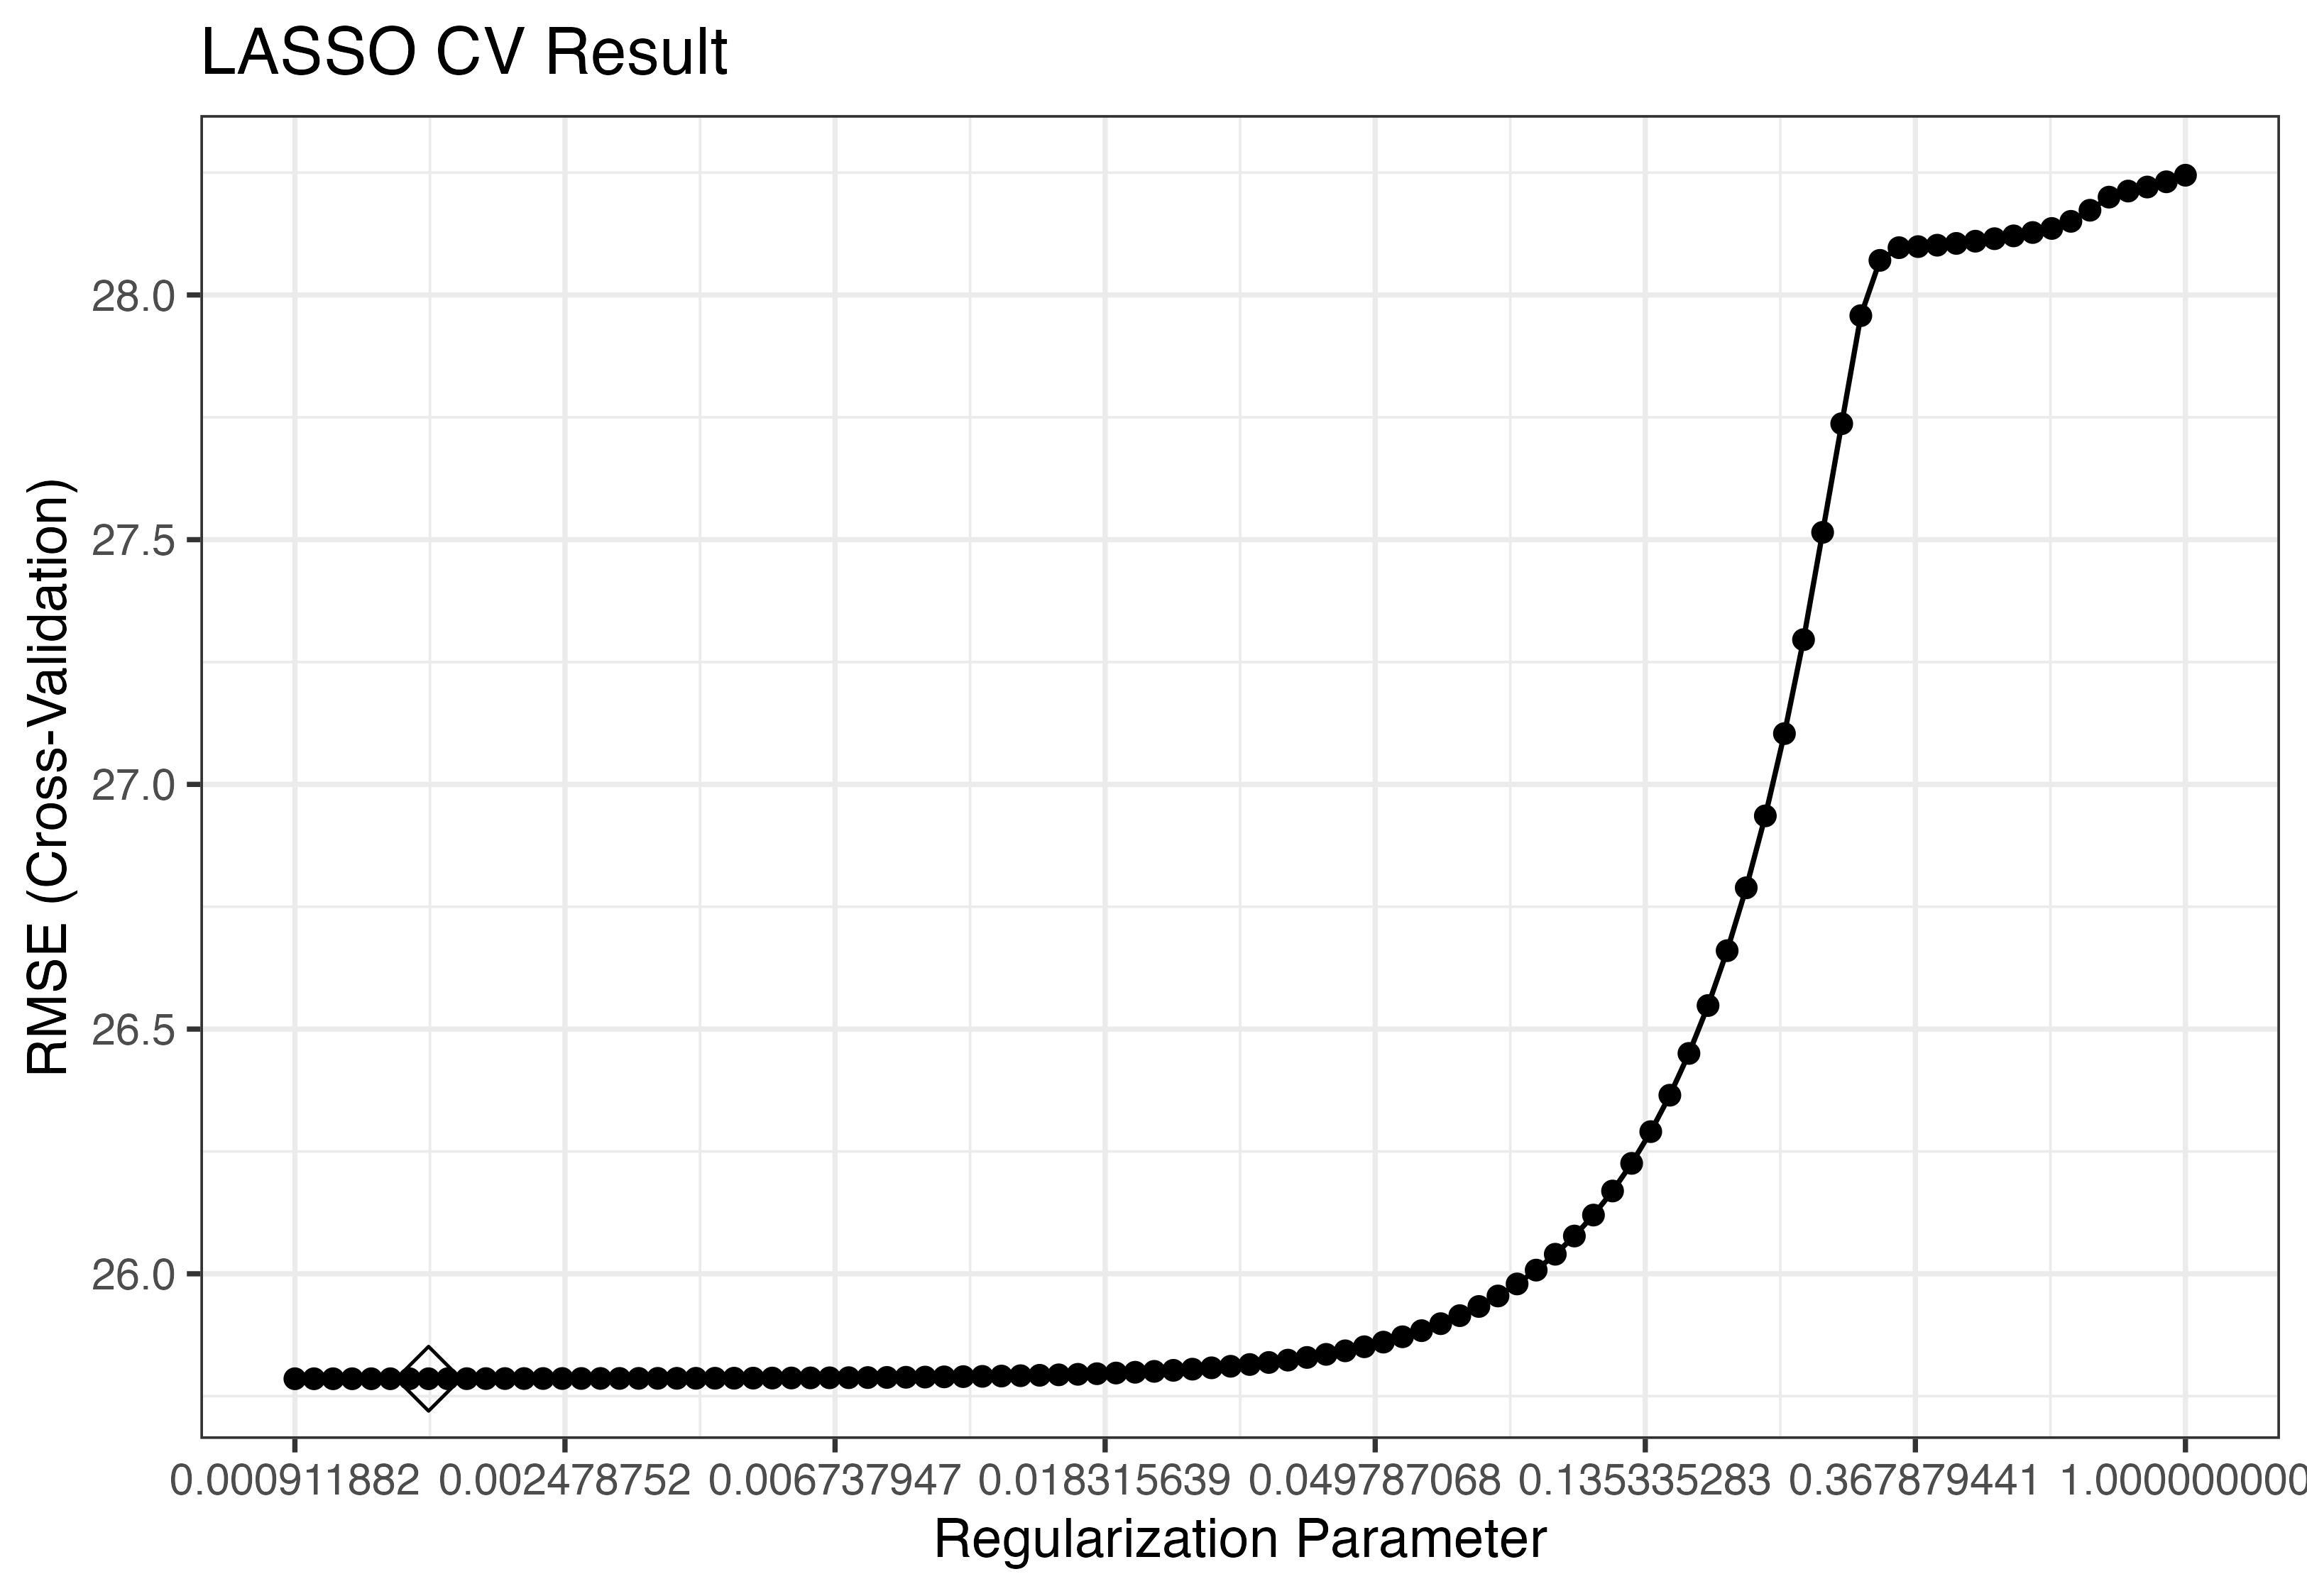
\includegraphics[width=0.32\textwidth]{primary/lasso_cv.jpeg}\label{fig:lasso}}
    \hspace{0.1cm}
    % 2
    \subfigure[Ridge]{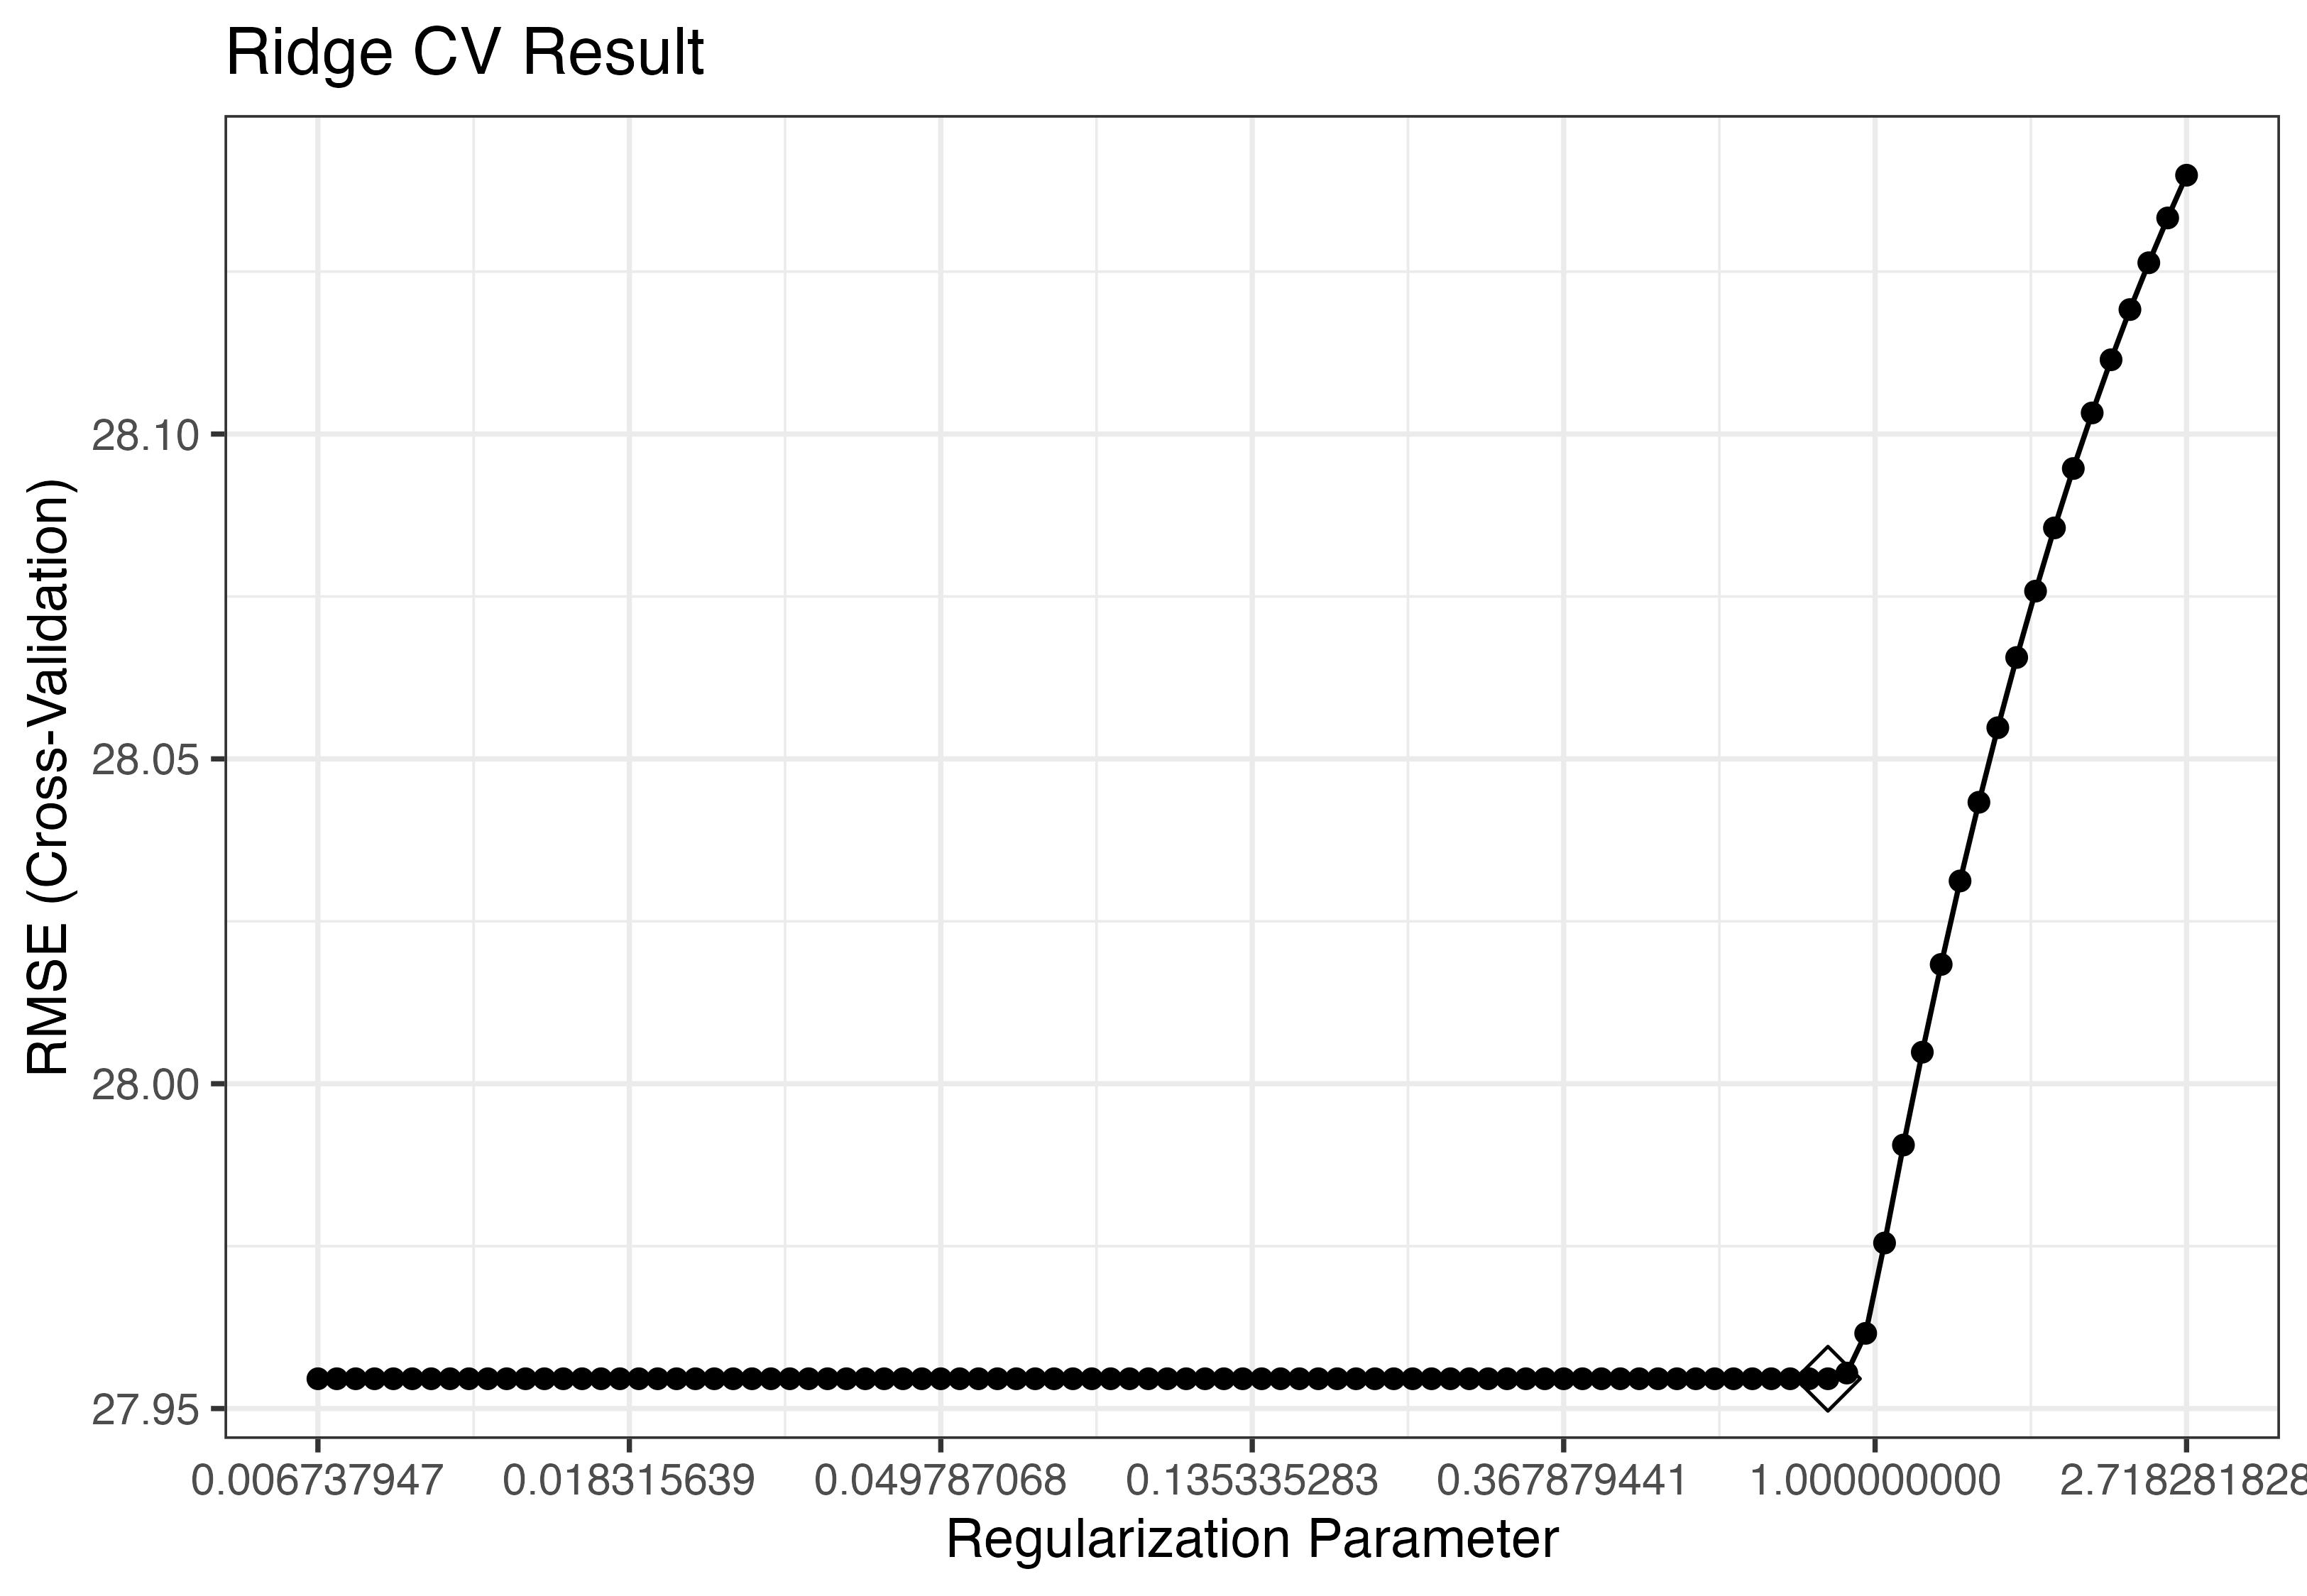
\includegraphics[width=0.32\textwidth]{primary/ridge_cv.jpeg}\label{fig:ridge}}
    \hspace{0.1cm}
    % 3
    \subfigure[Elastic net]{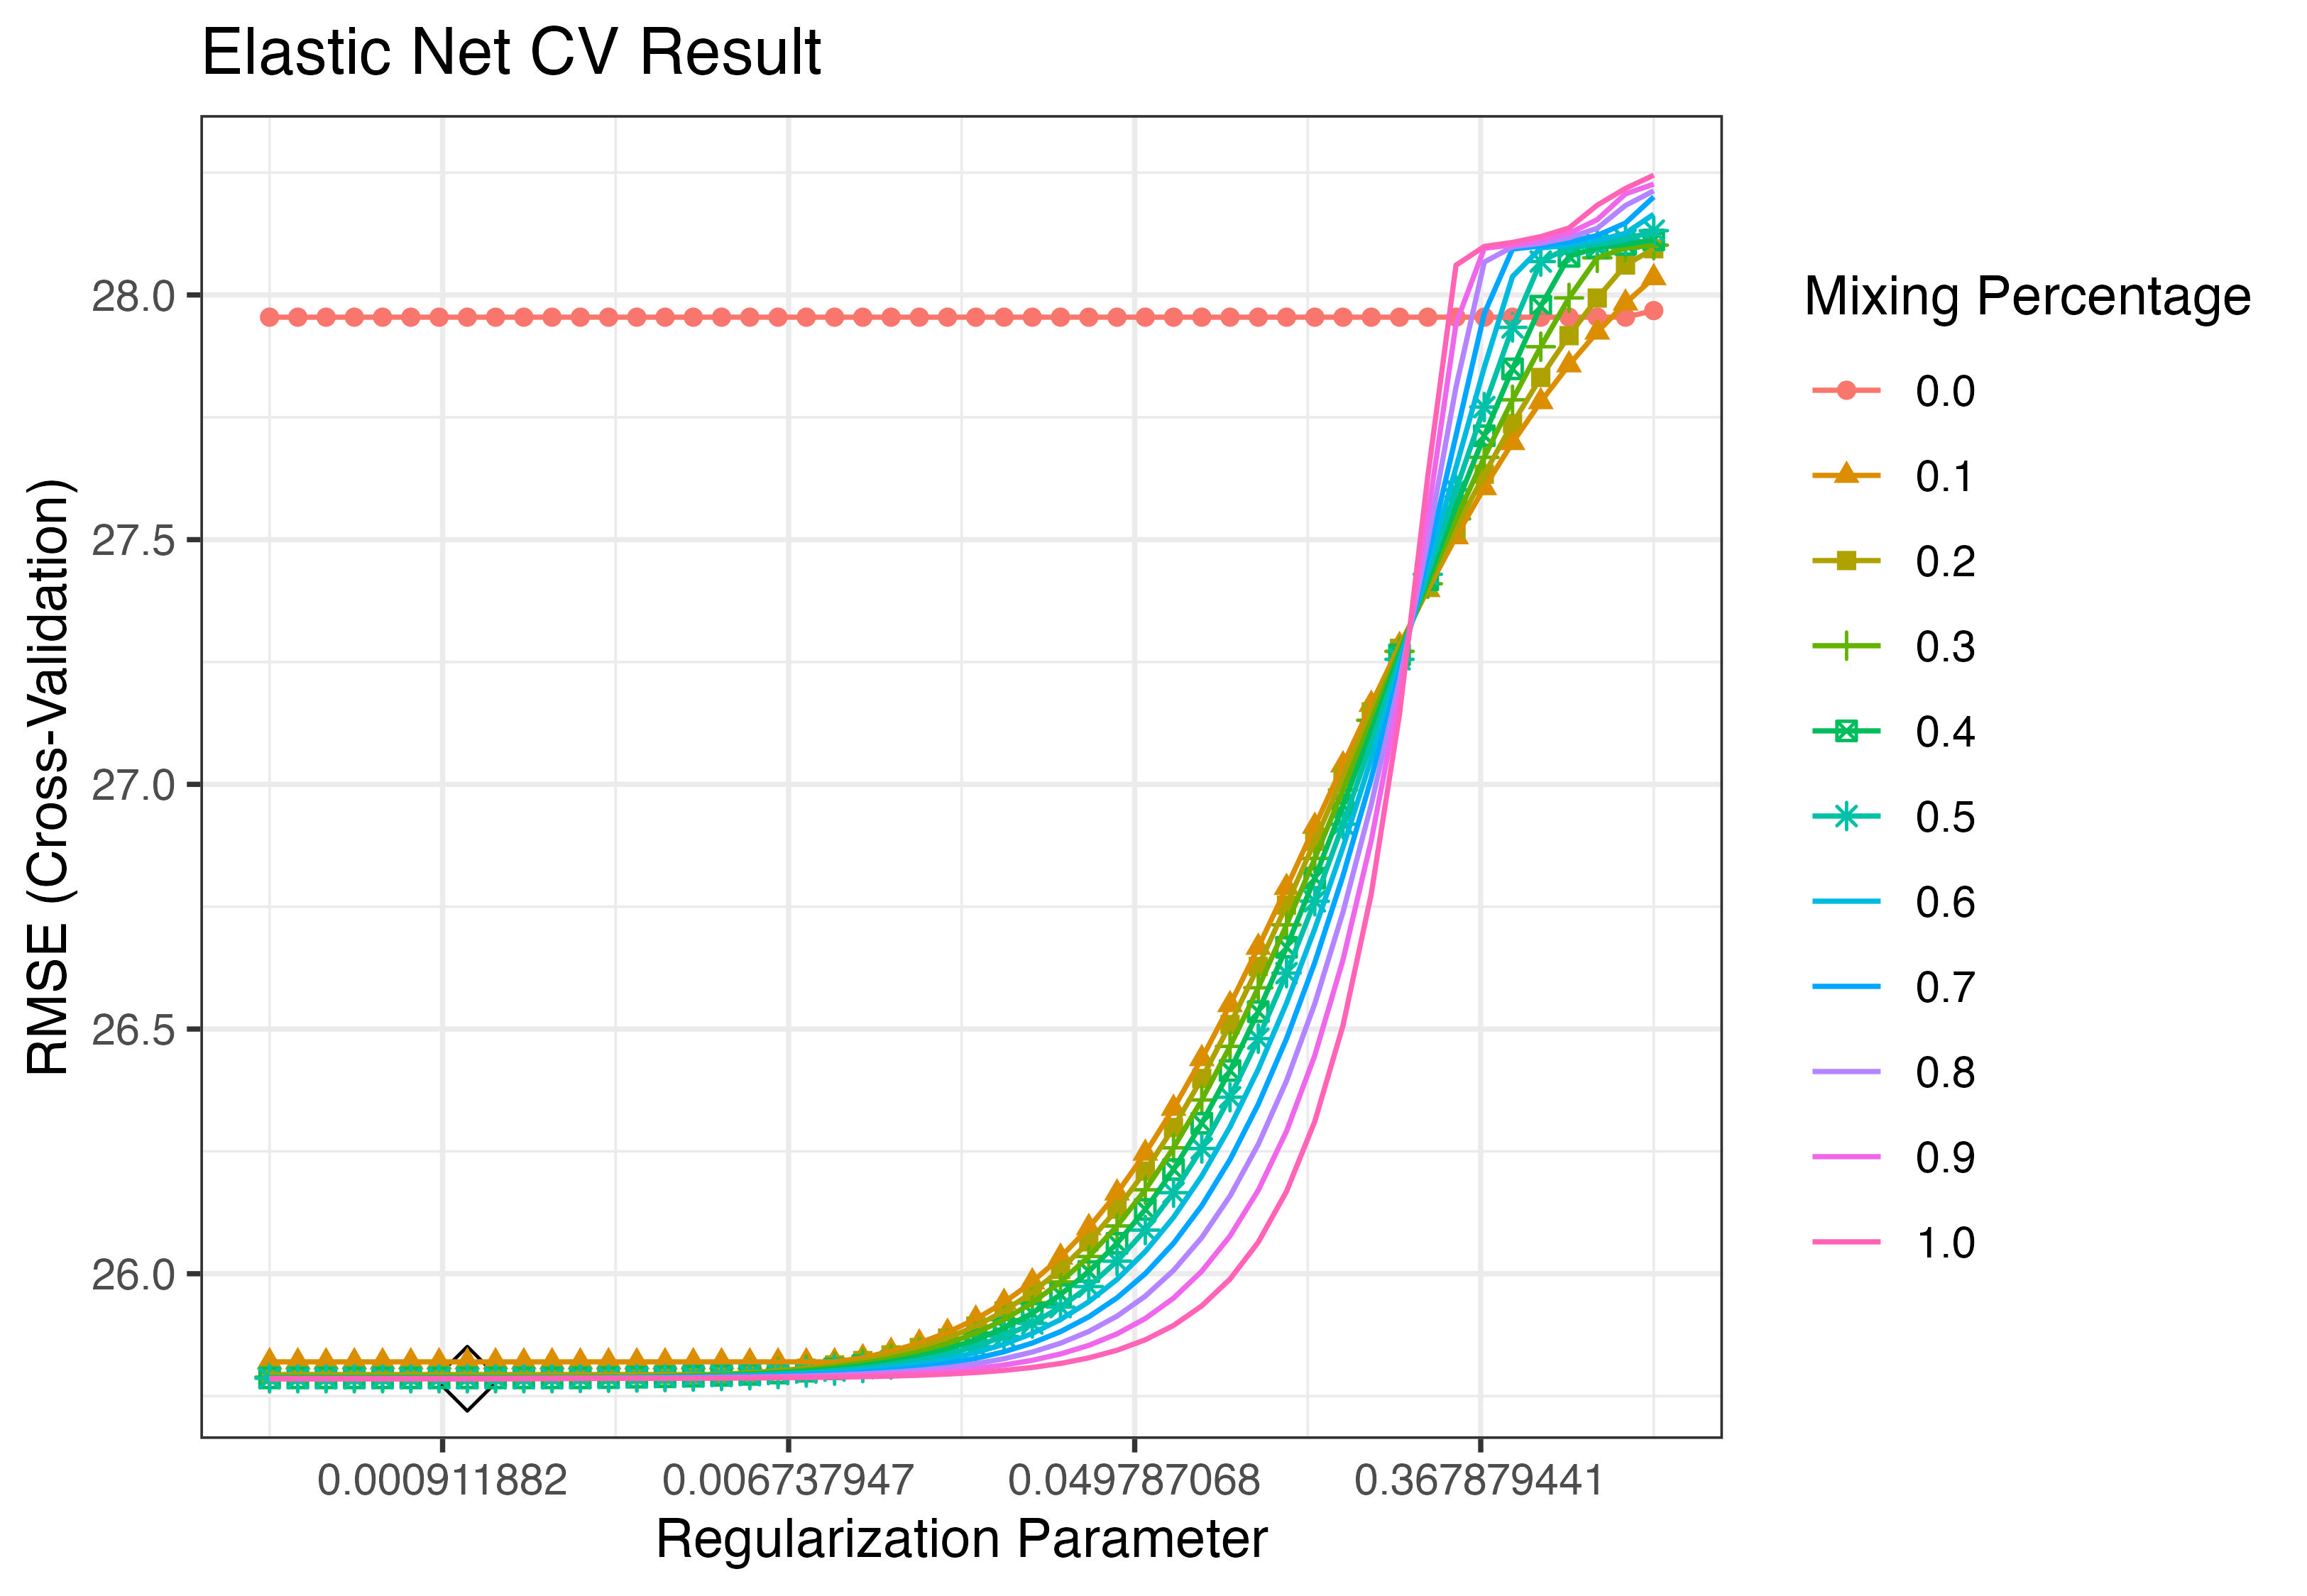
\includegraphics[width=0.32\textwidth]{primary/enet_cv.jpeg}\label{fig:enet}}

    % 1
    \subfigure[PCR]{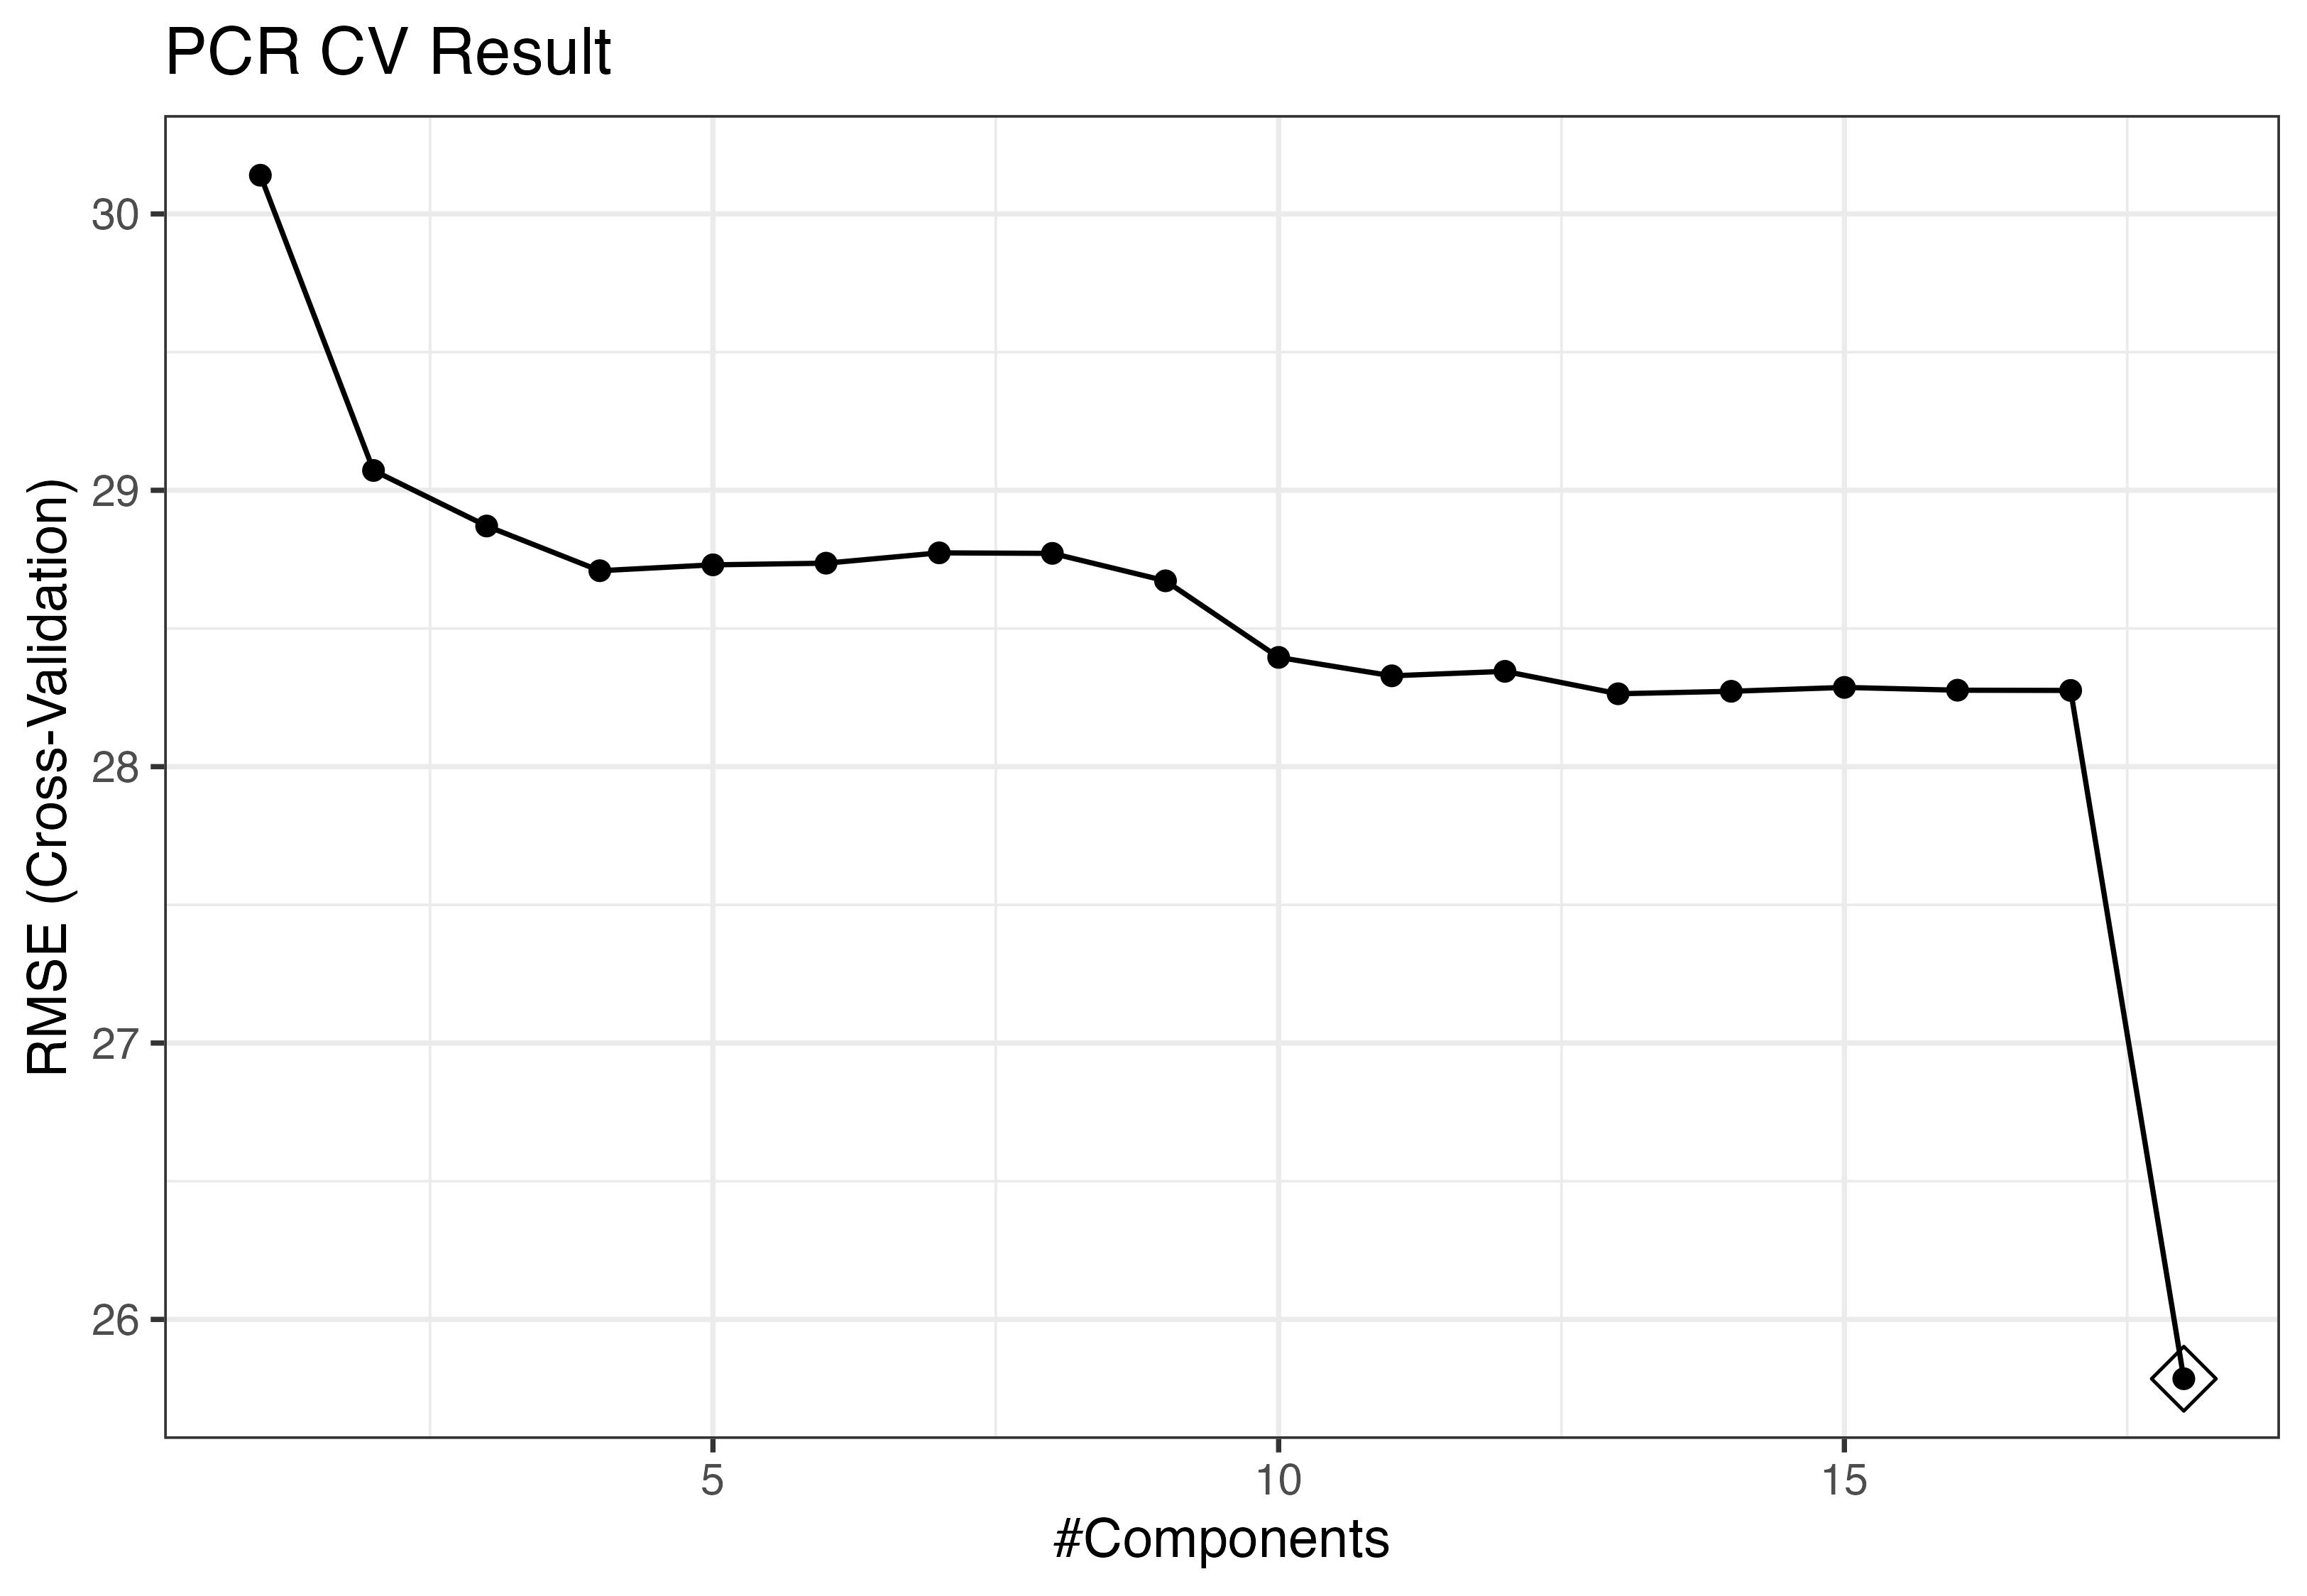
\includegraphics[width=0.32\textwidth]{primary/pcr_cv.jpeg}\label{fig:pcr}}
    \hspace{0.1cm}
    % 2
    \subfigure[PLS]{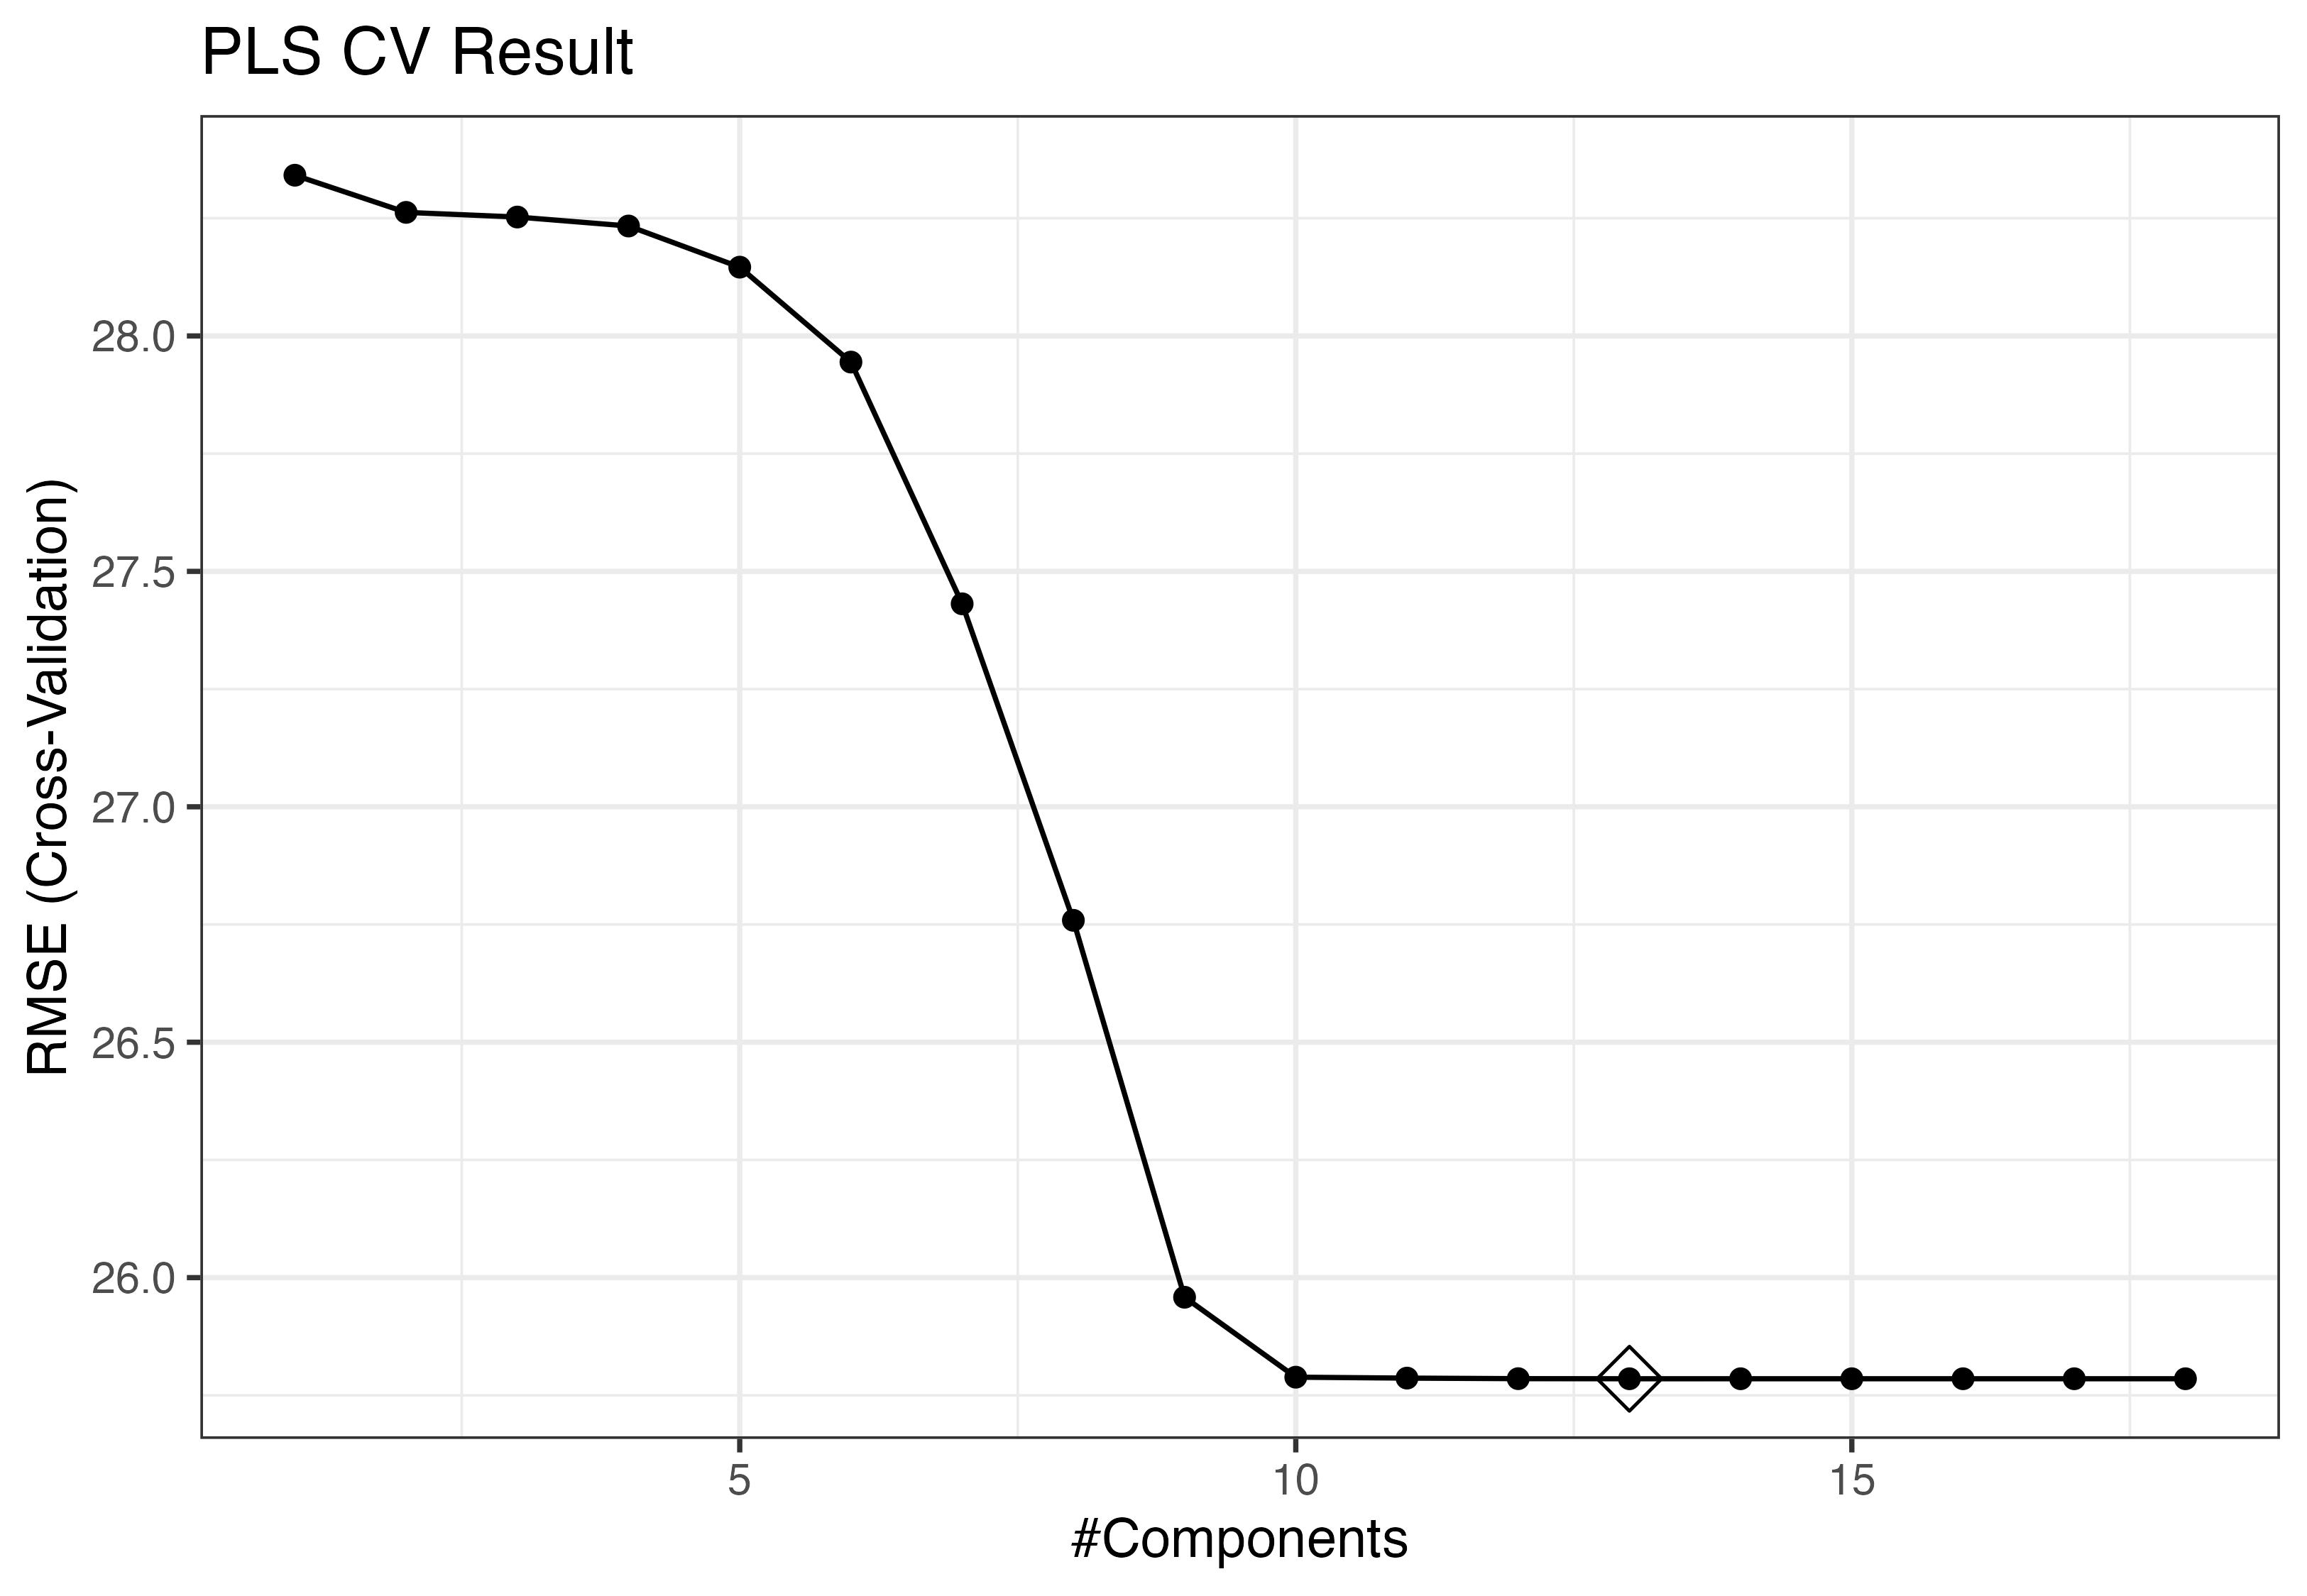
\includegraphics[width=0.32\textwidth]{primary/pls_cv.jpeg}\label{fig:pls}}
    \hspace{0.1cm}
    % 3
    \subfigure[GAM]{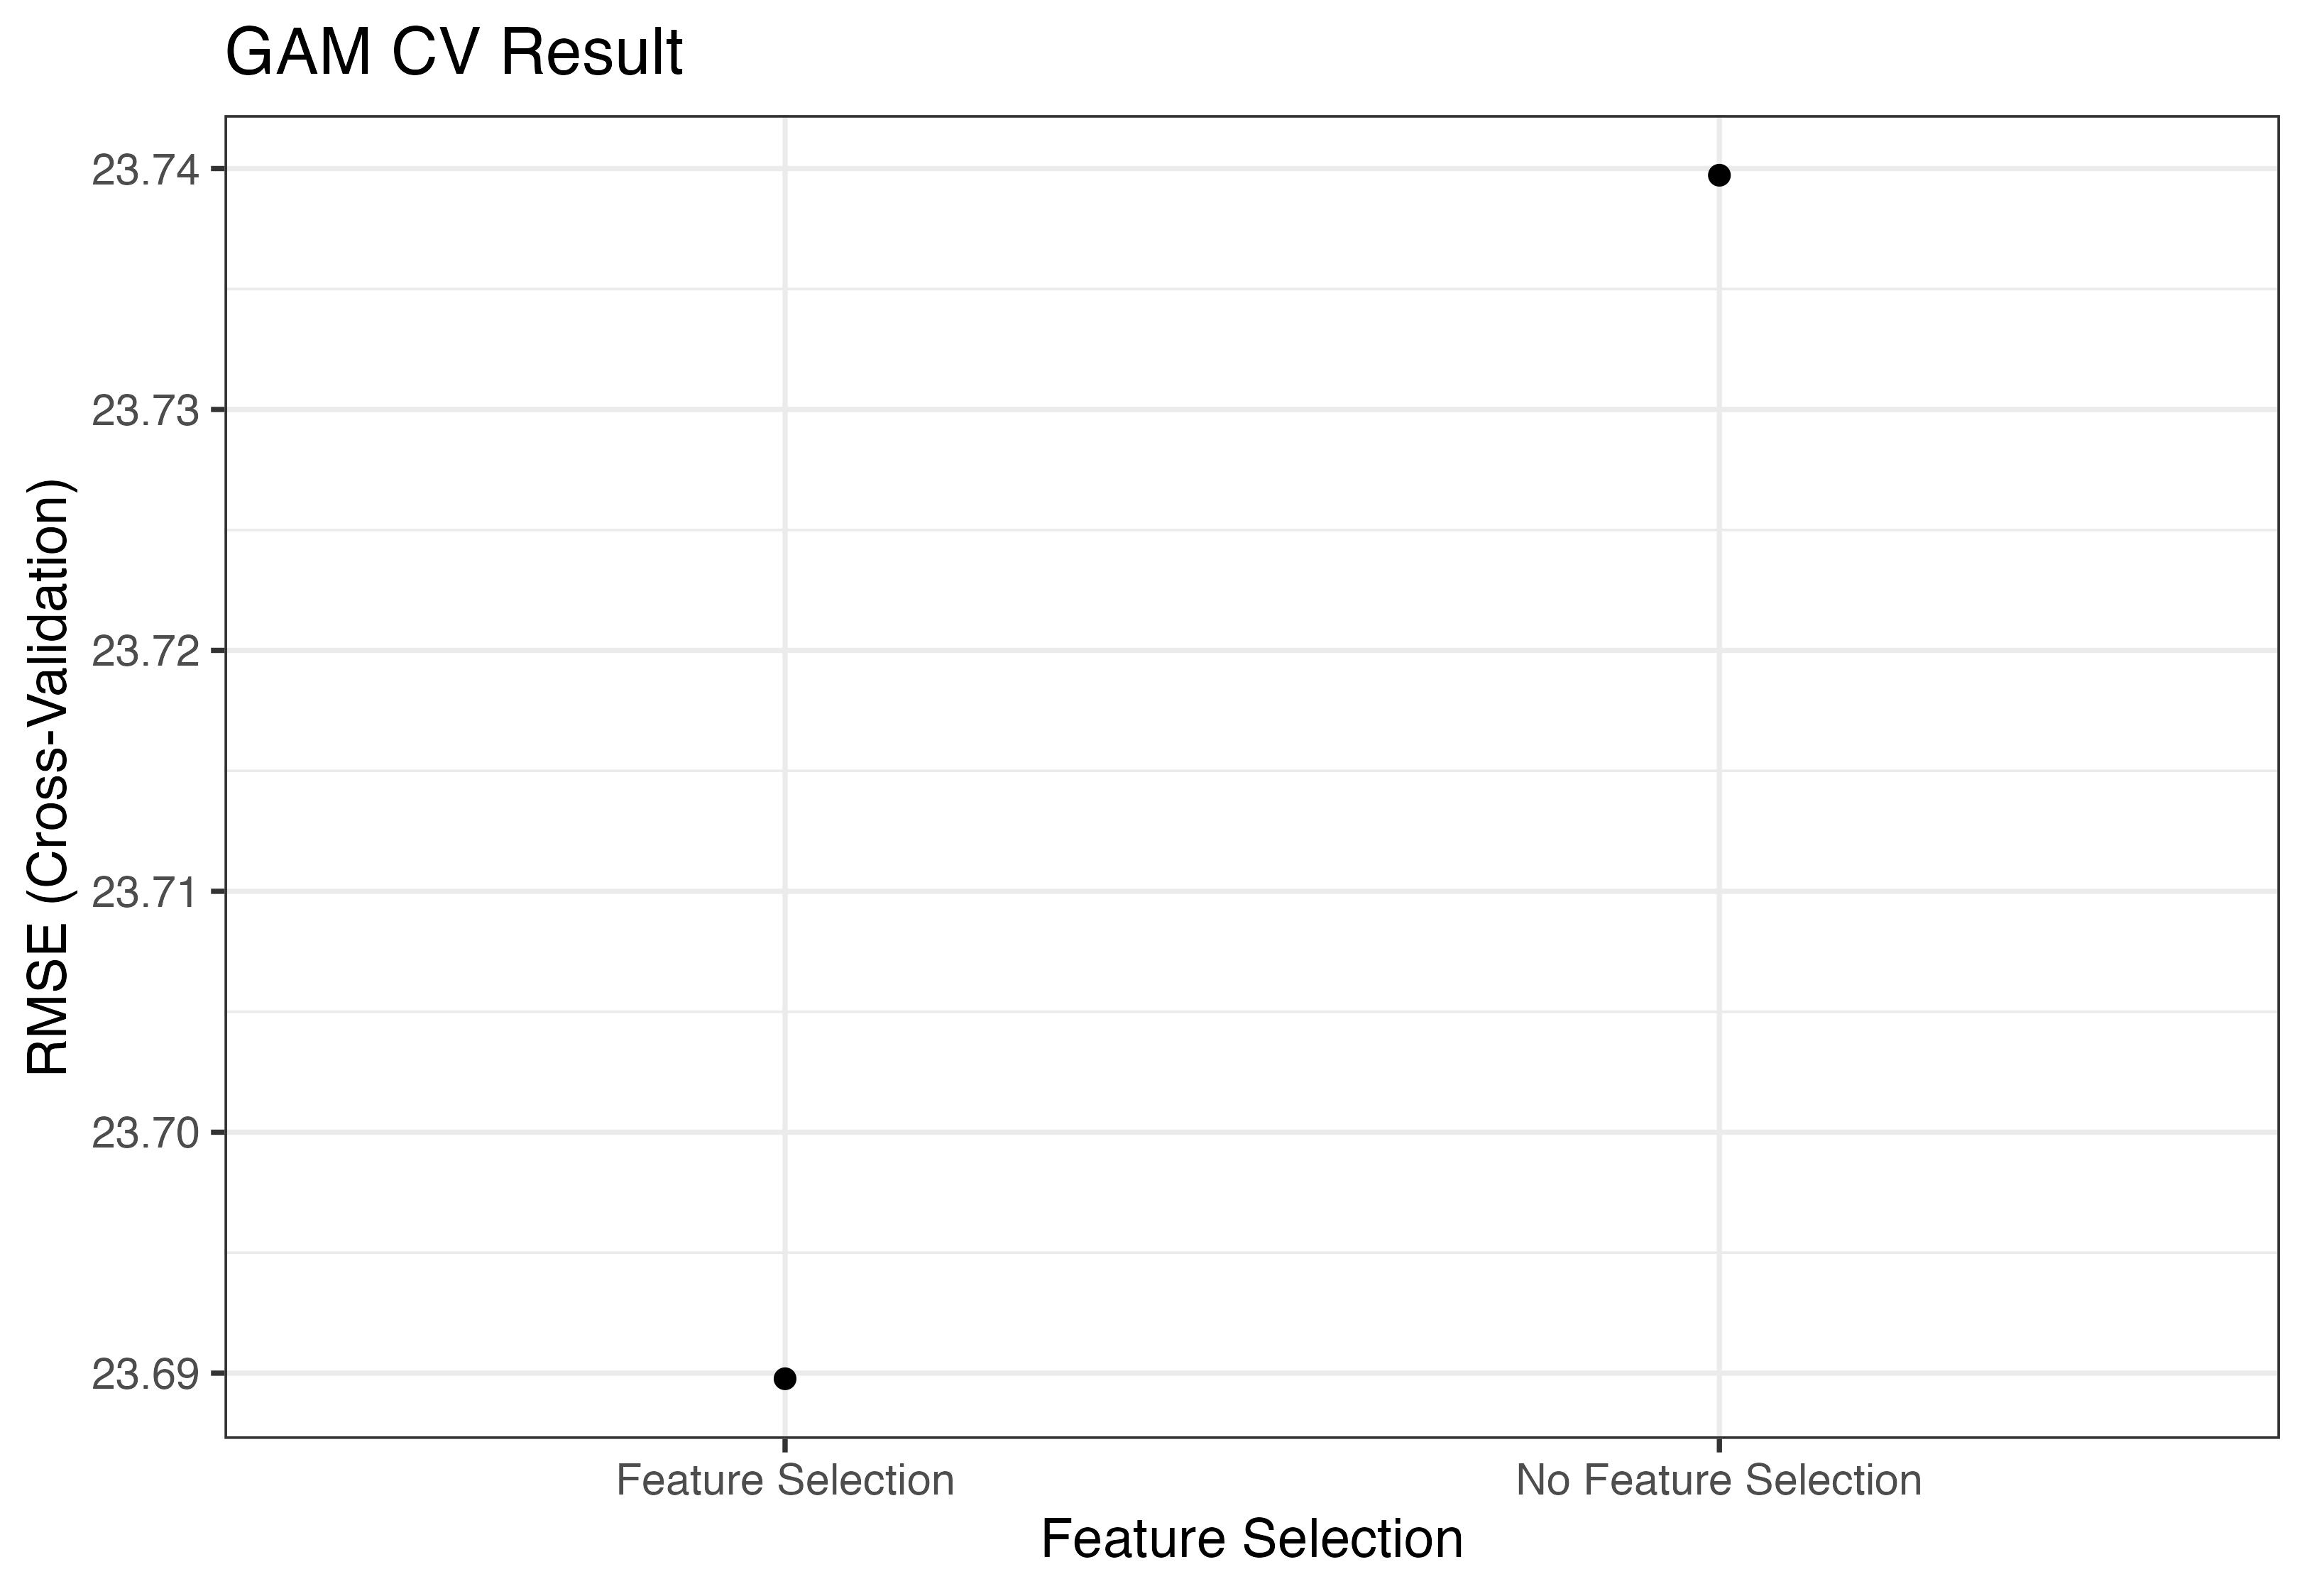
\includegraphics[width=0.32\textwidth]{primary/gam_cv.jpeg}\label{fig:gam}}

    % 1
    \subfigure[MARS]{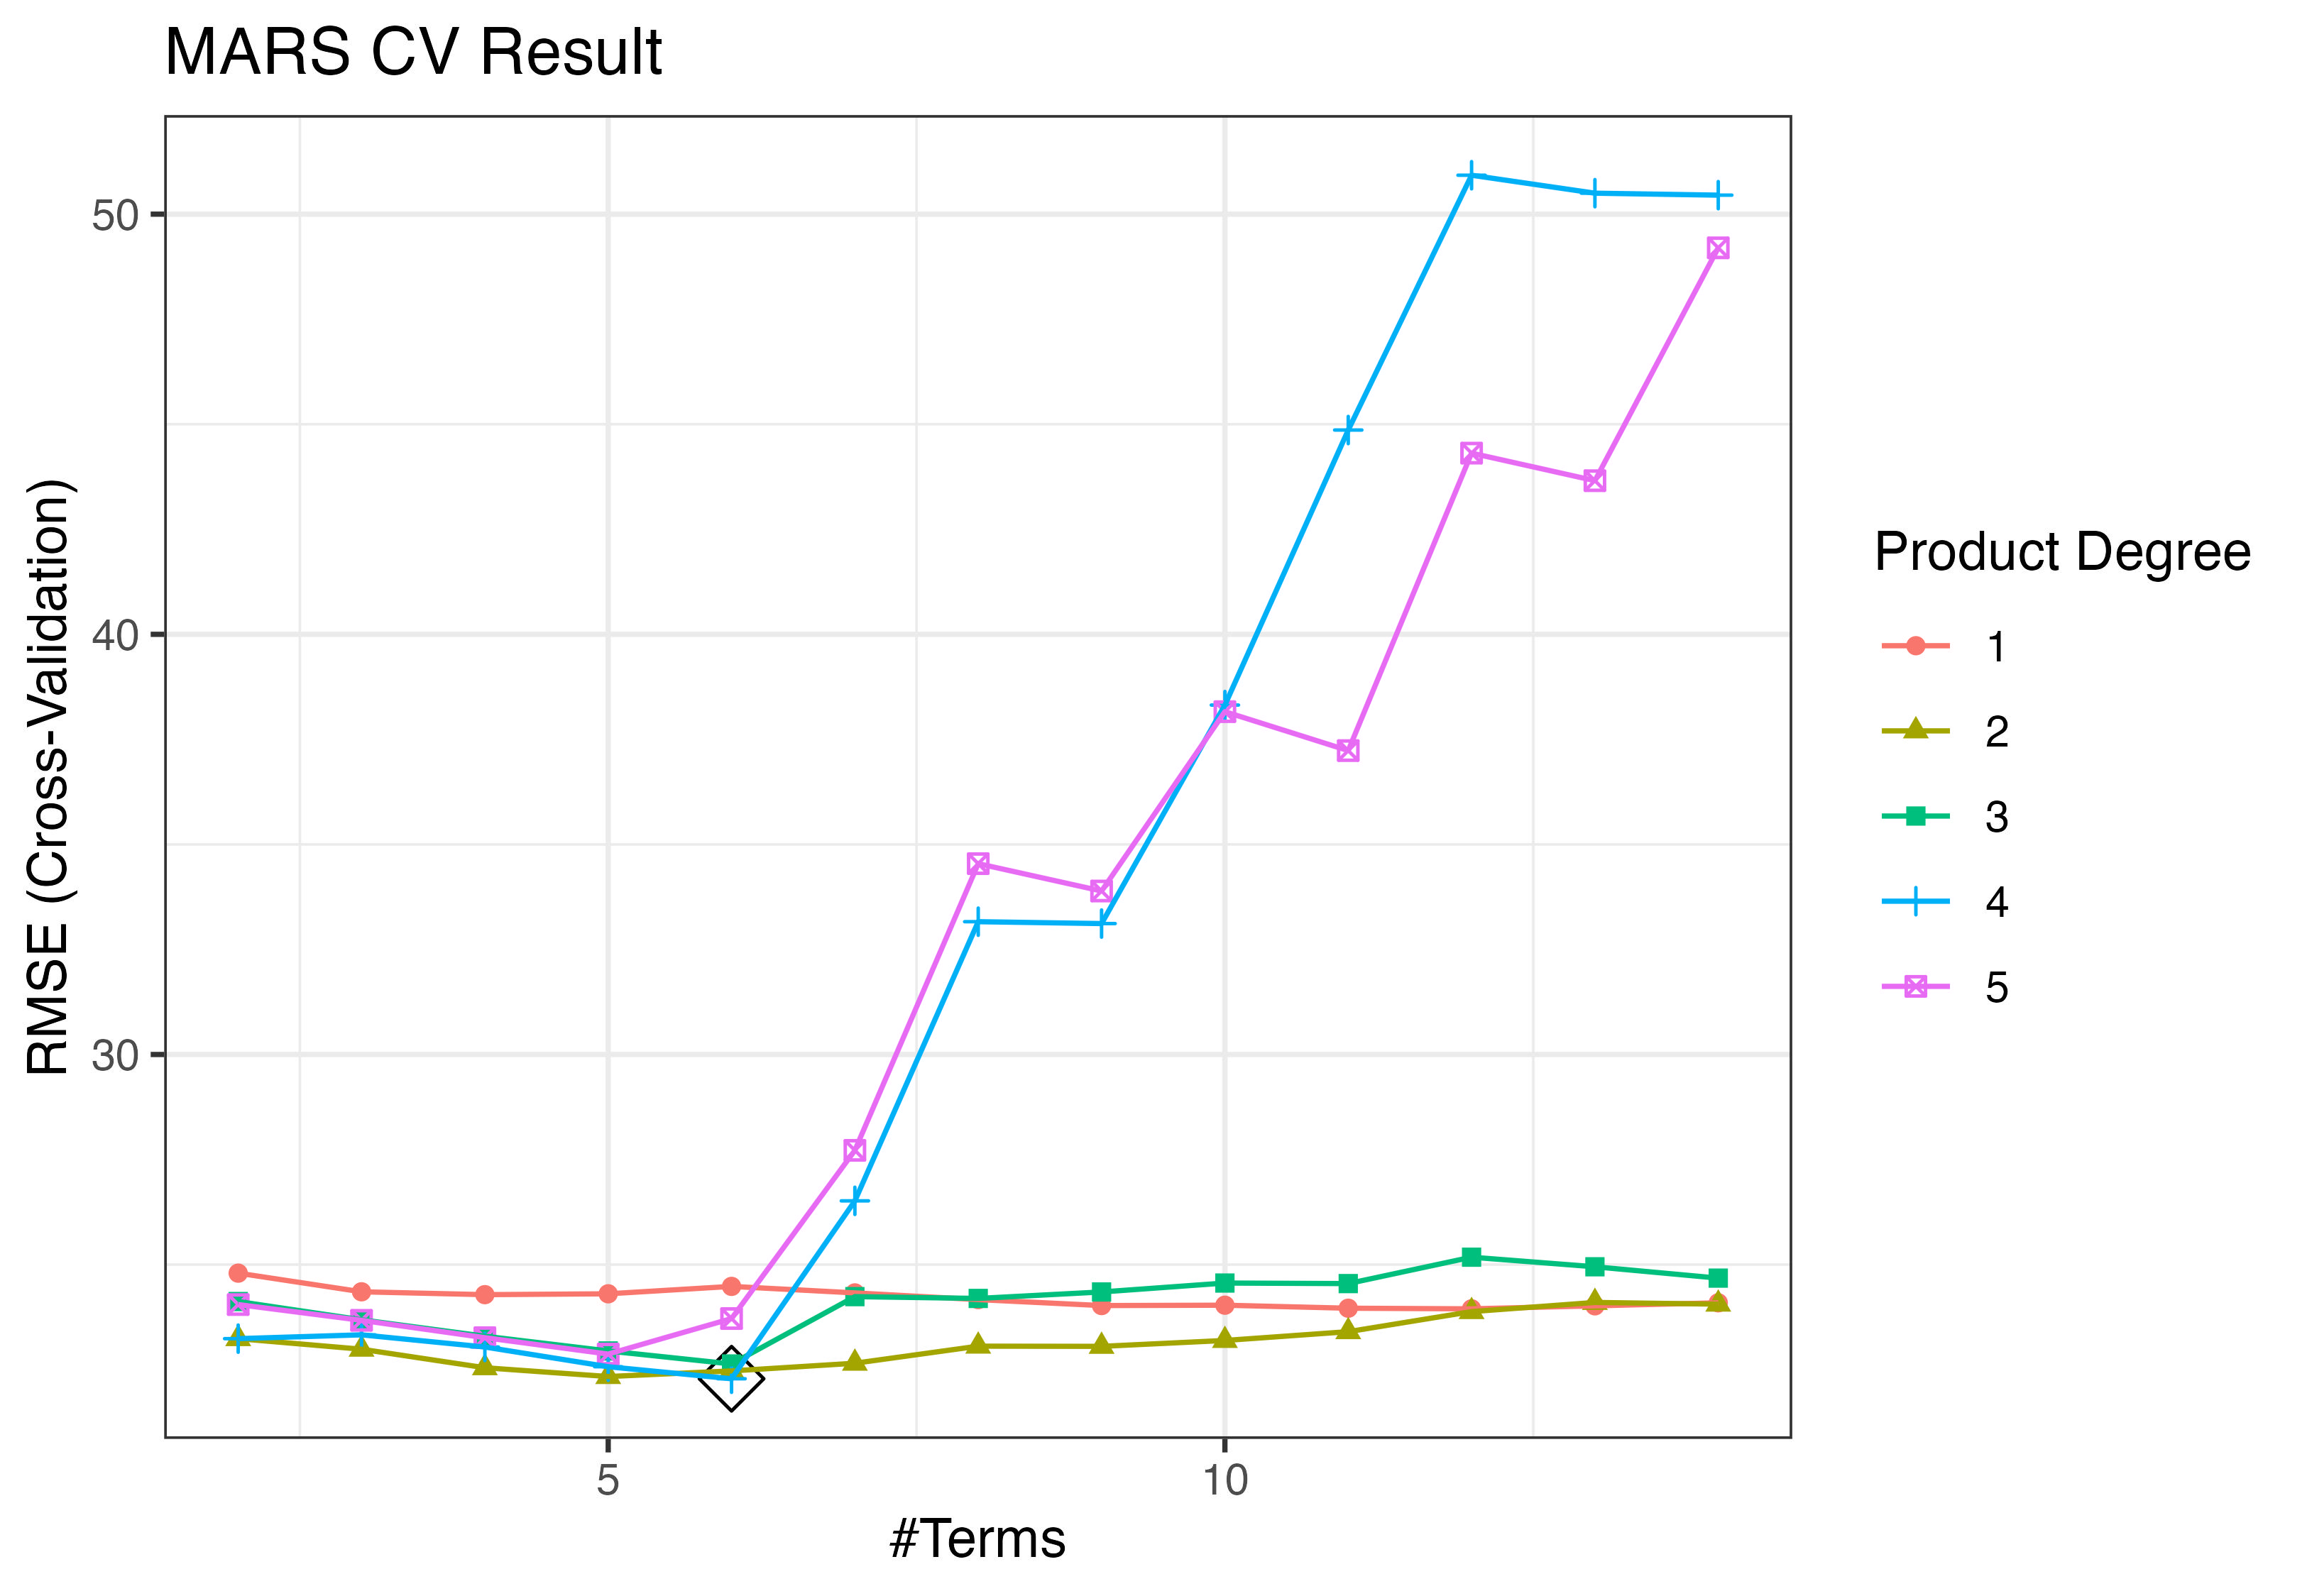
\includegraphics[width=0.32\textwidth]{primary/mars_cv.jpeg}\label{fig:mars}}
    \hspace{0.1cm}
    % 2
    \subfigure[KNN]{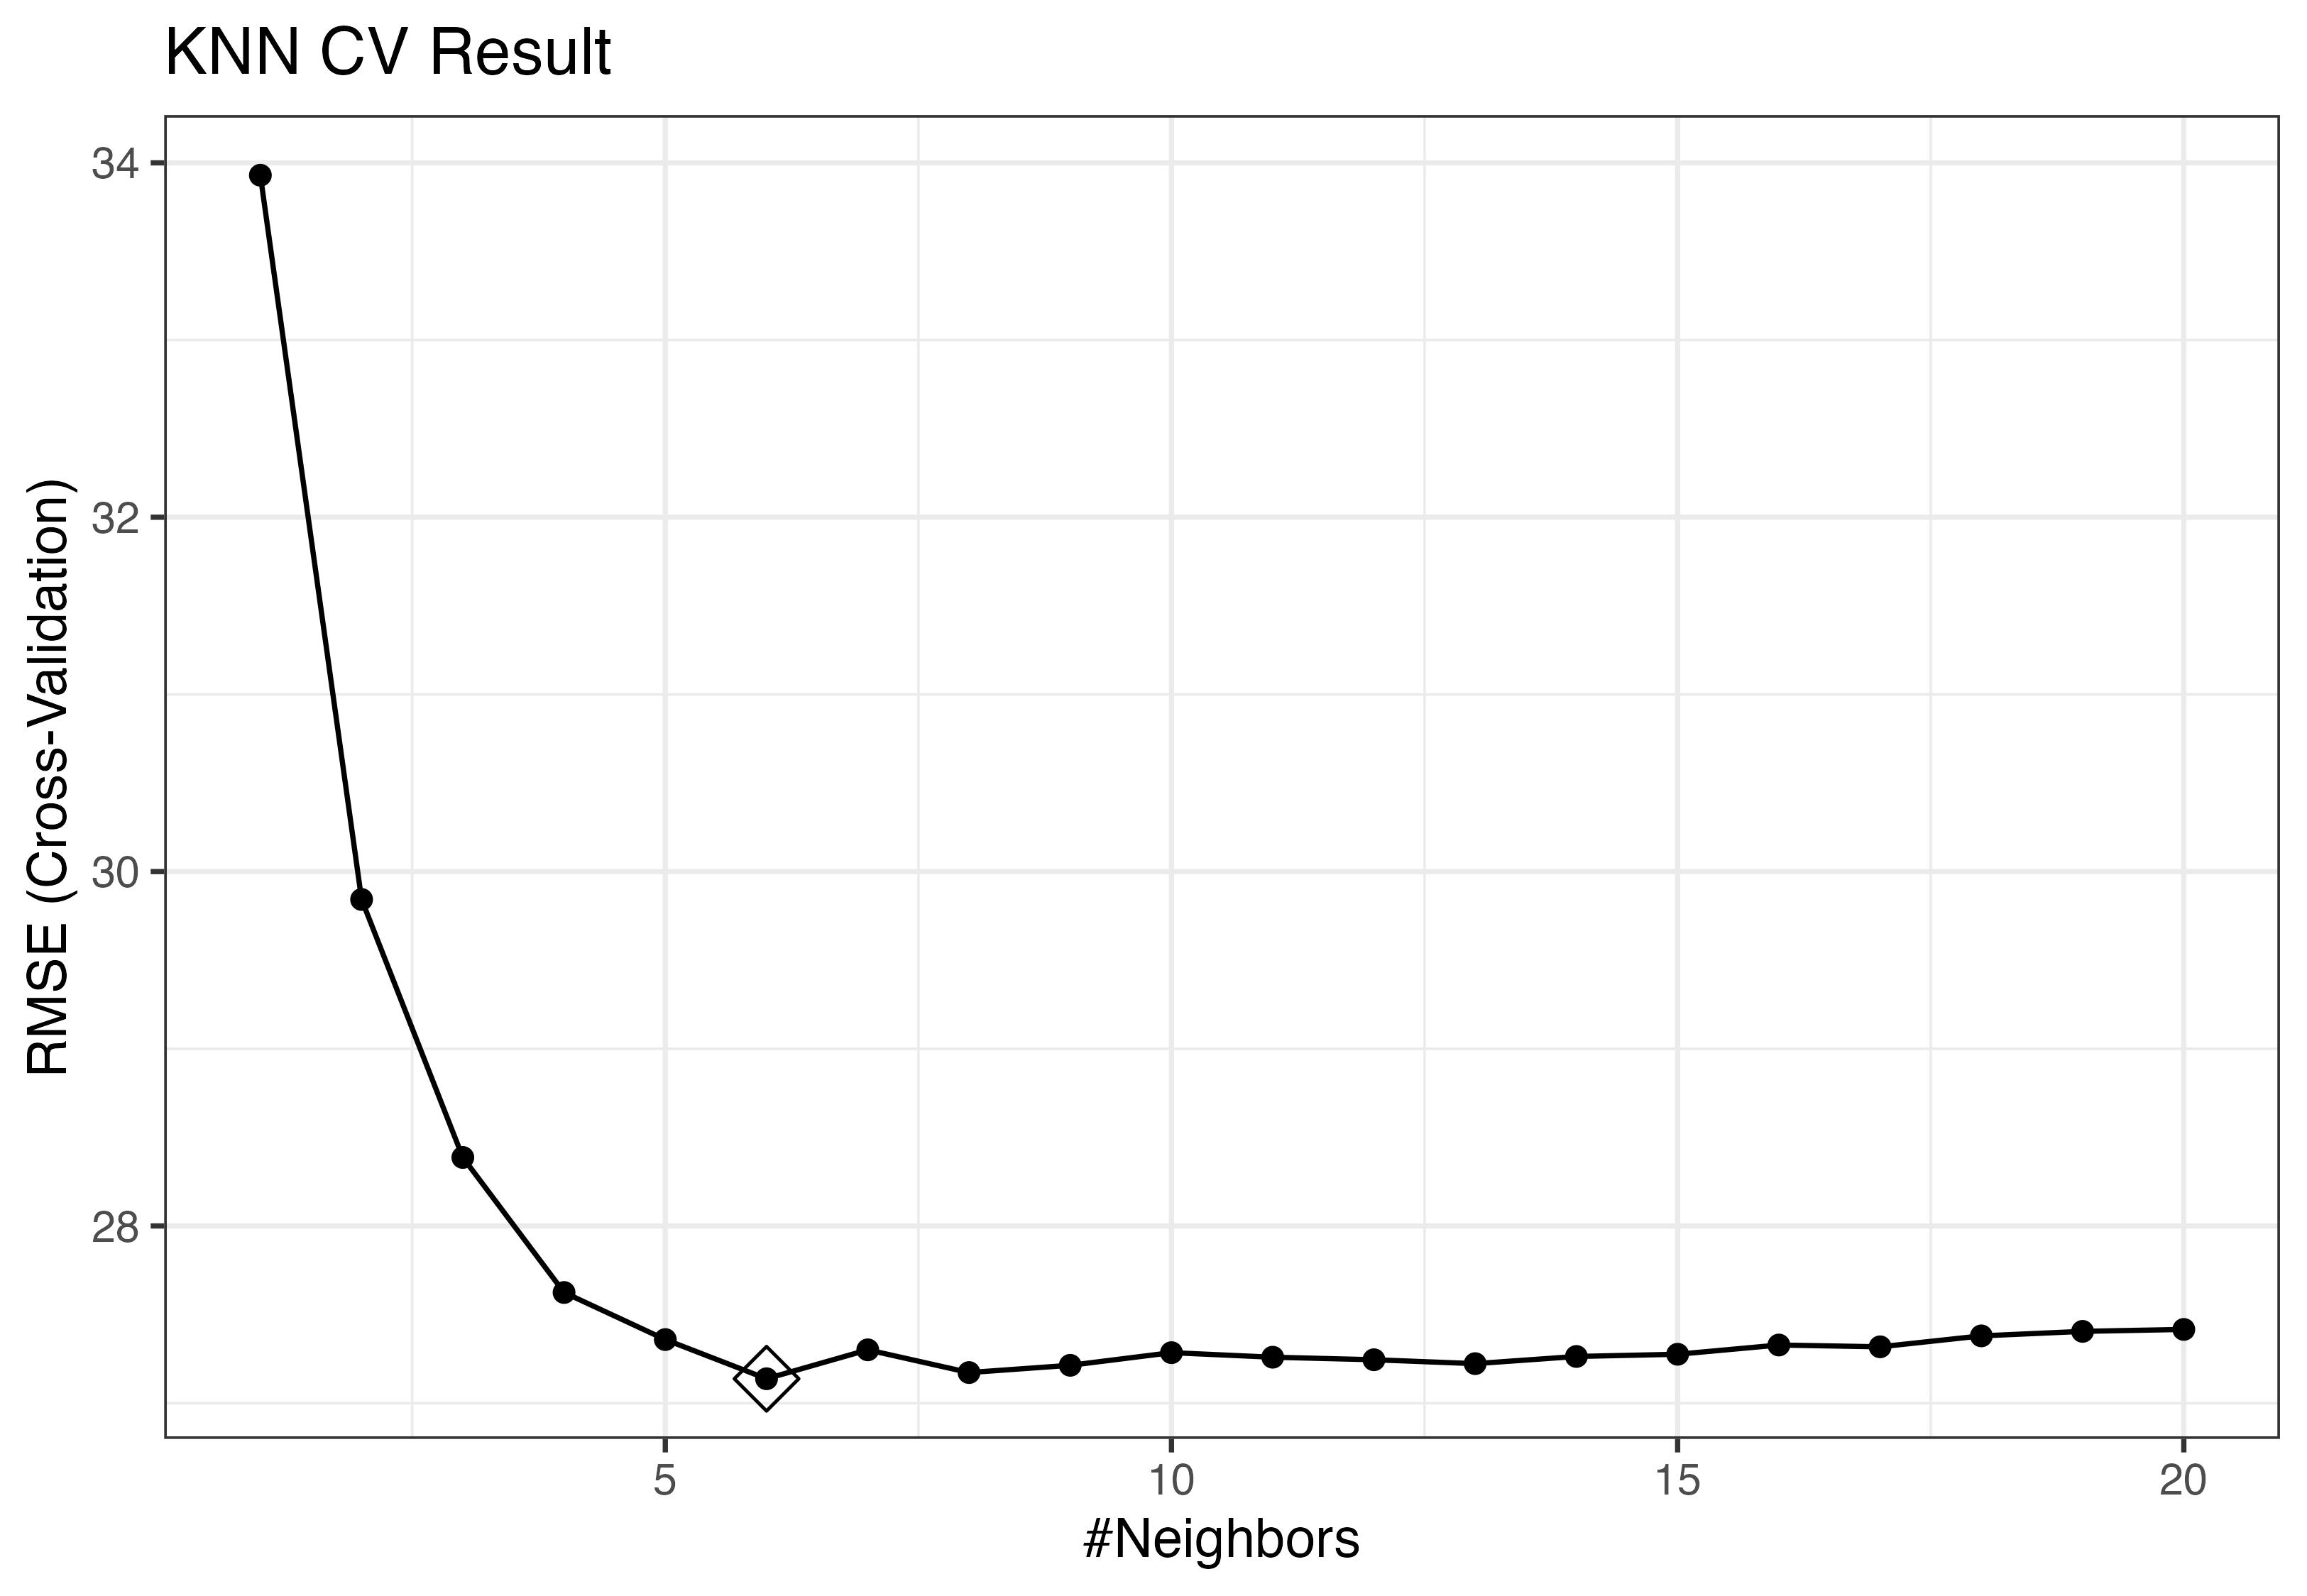
\includegraphics[width=0.32\textwidth]{primary/knn_cv.jpeg}\label{fig:knn}}
    \hspace{0.1cm}
    % 3
    \subfigure[Bagging]{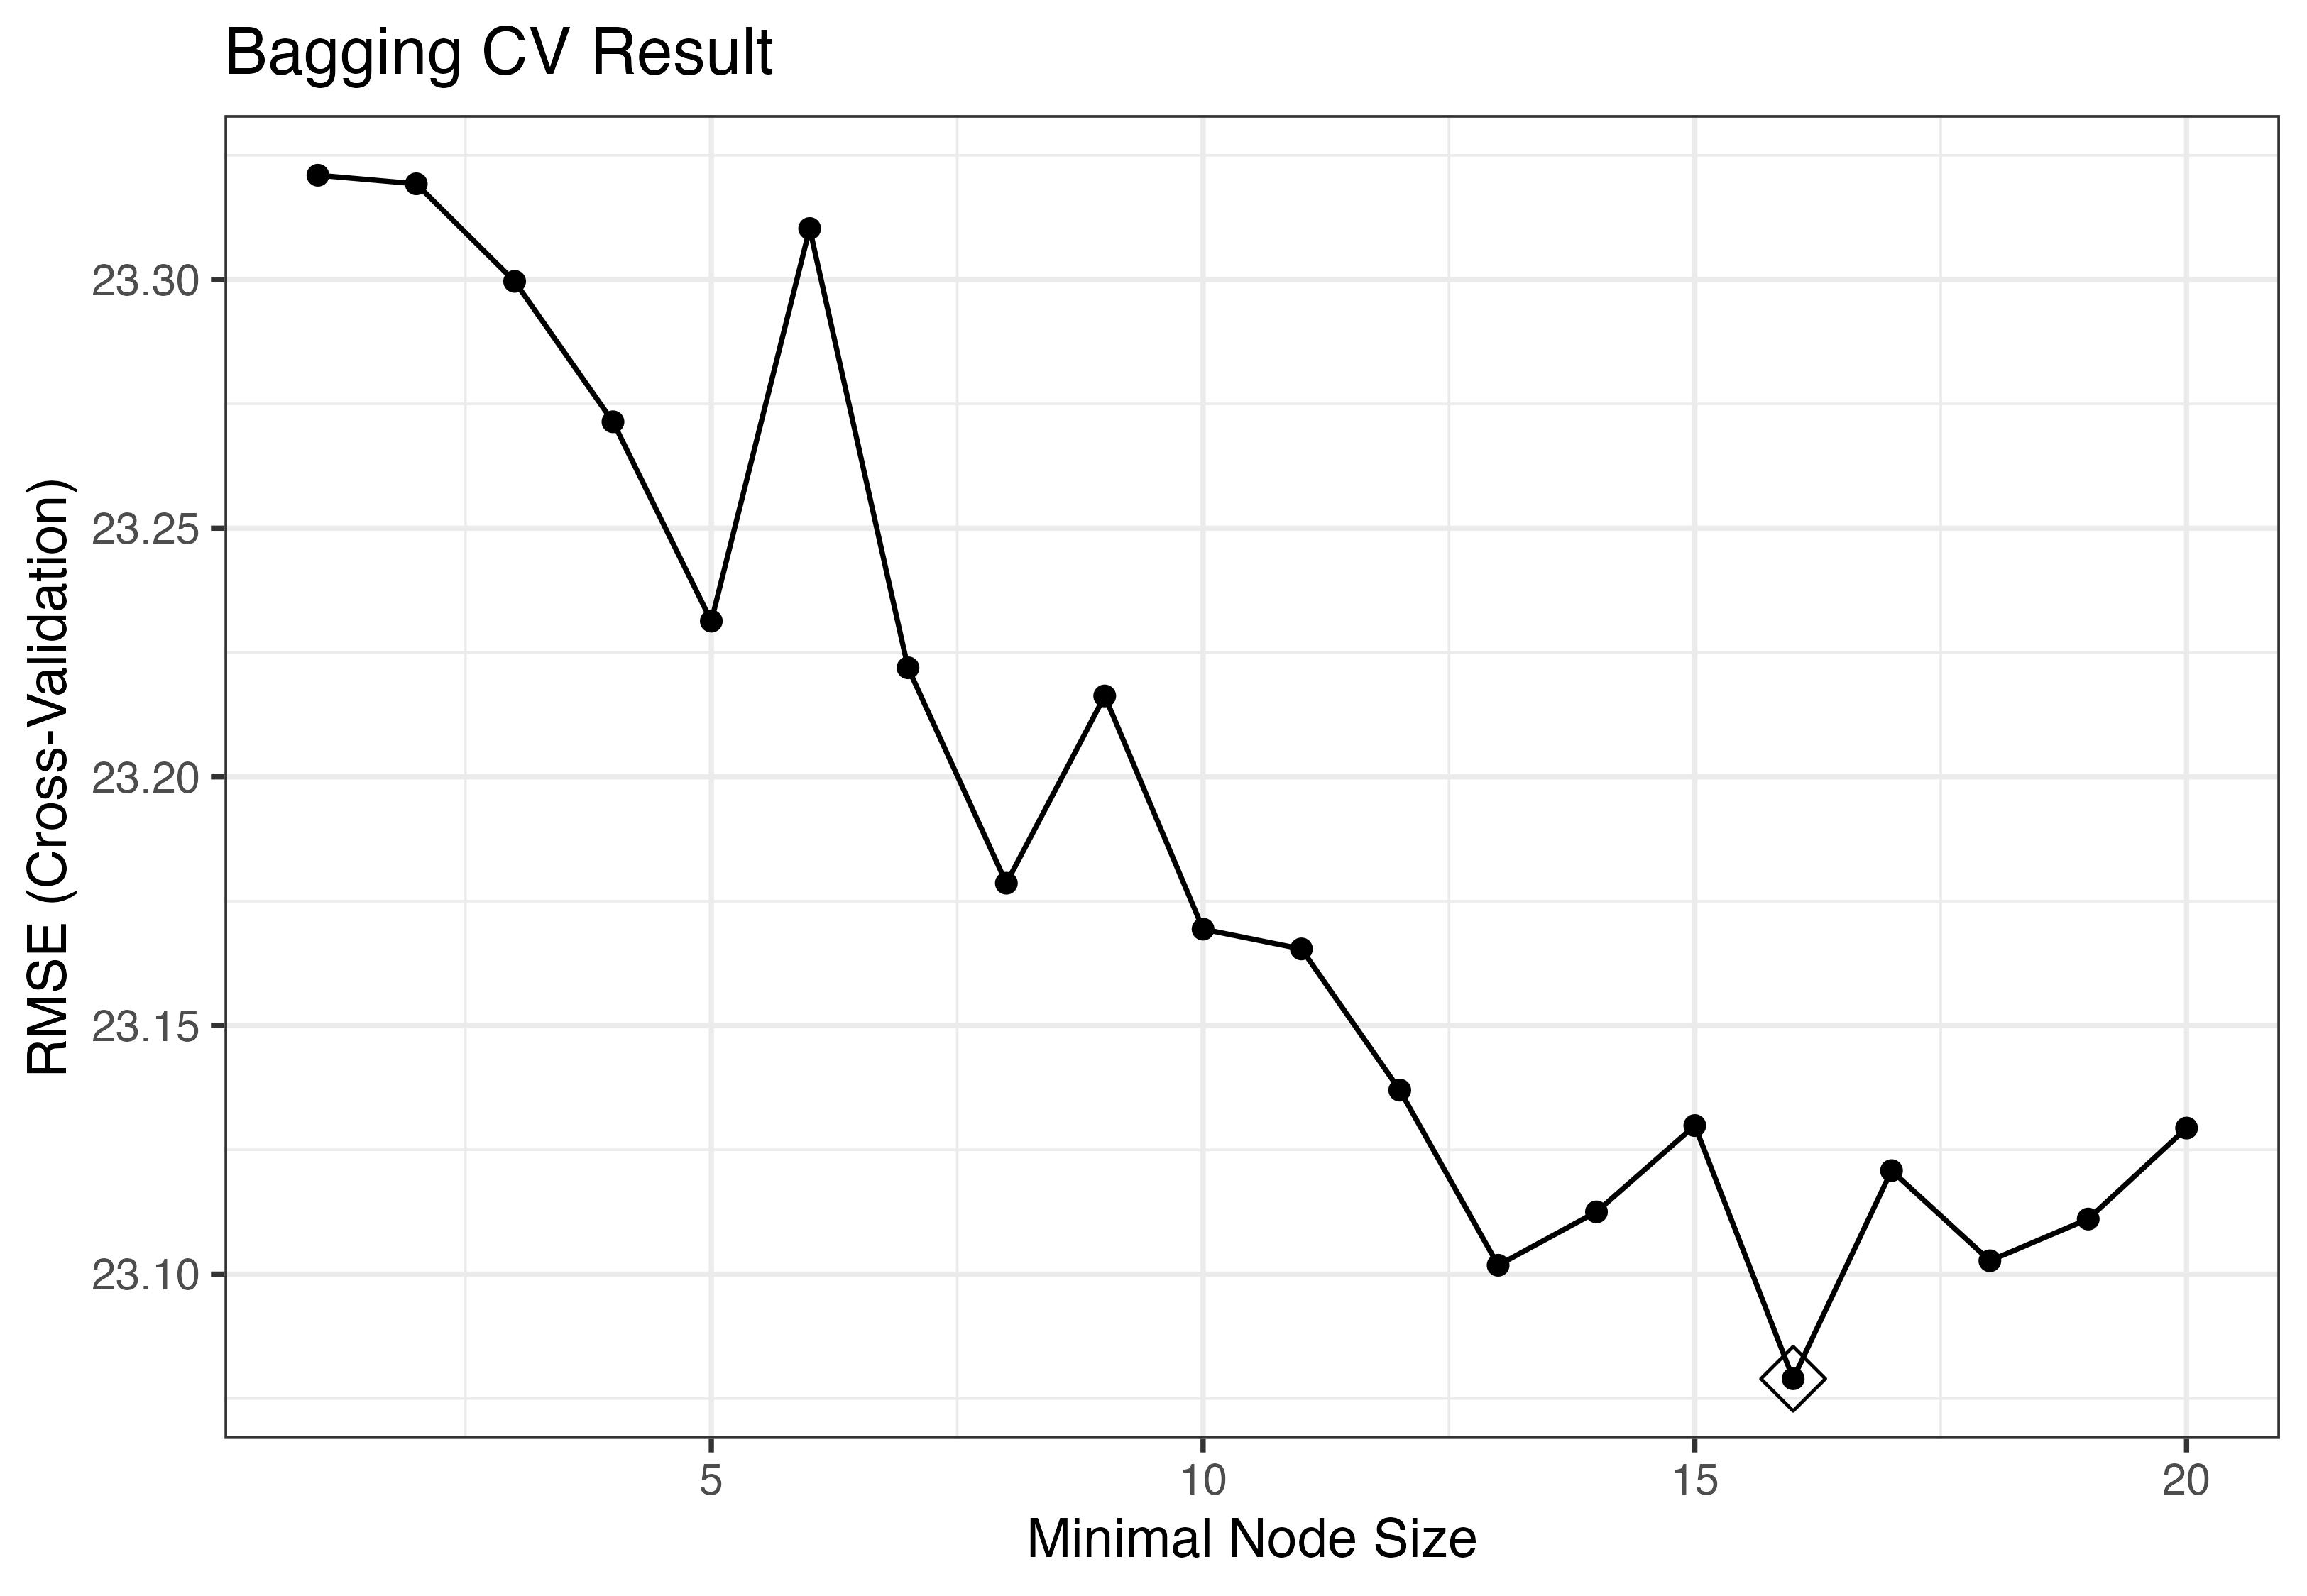
\includegraphics[width=0.32\textwidth]{primary/bagging_cv.jpeg}\label{fig:bagging}}

    % 1
    \subfigure[Random Forest]{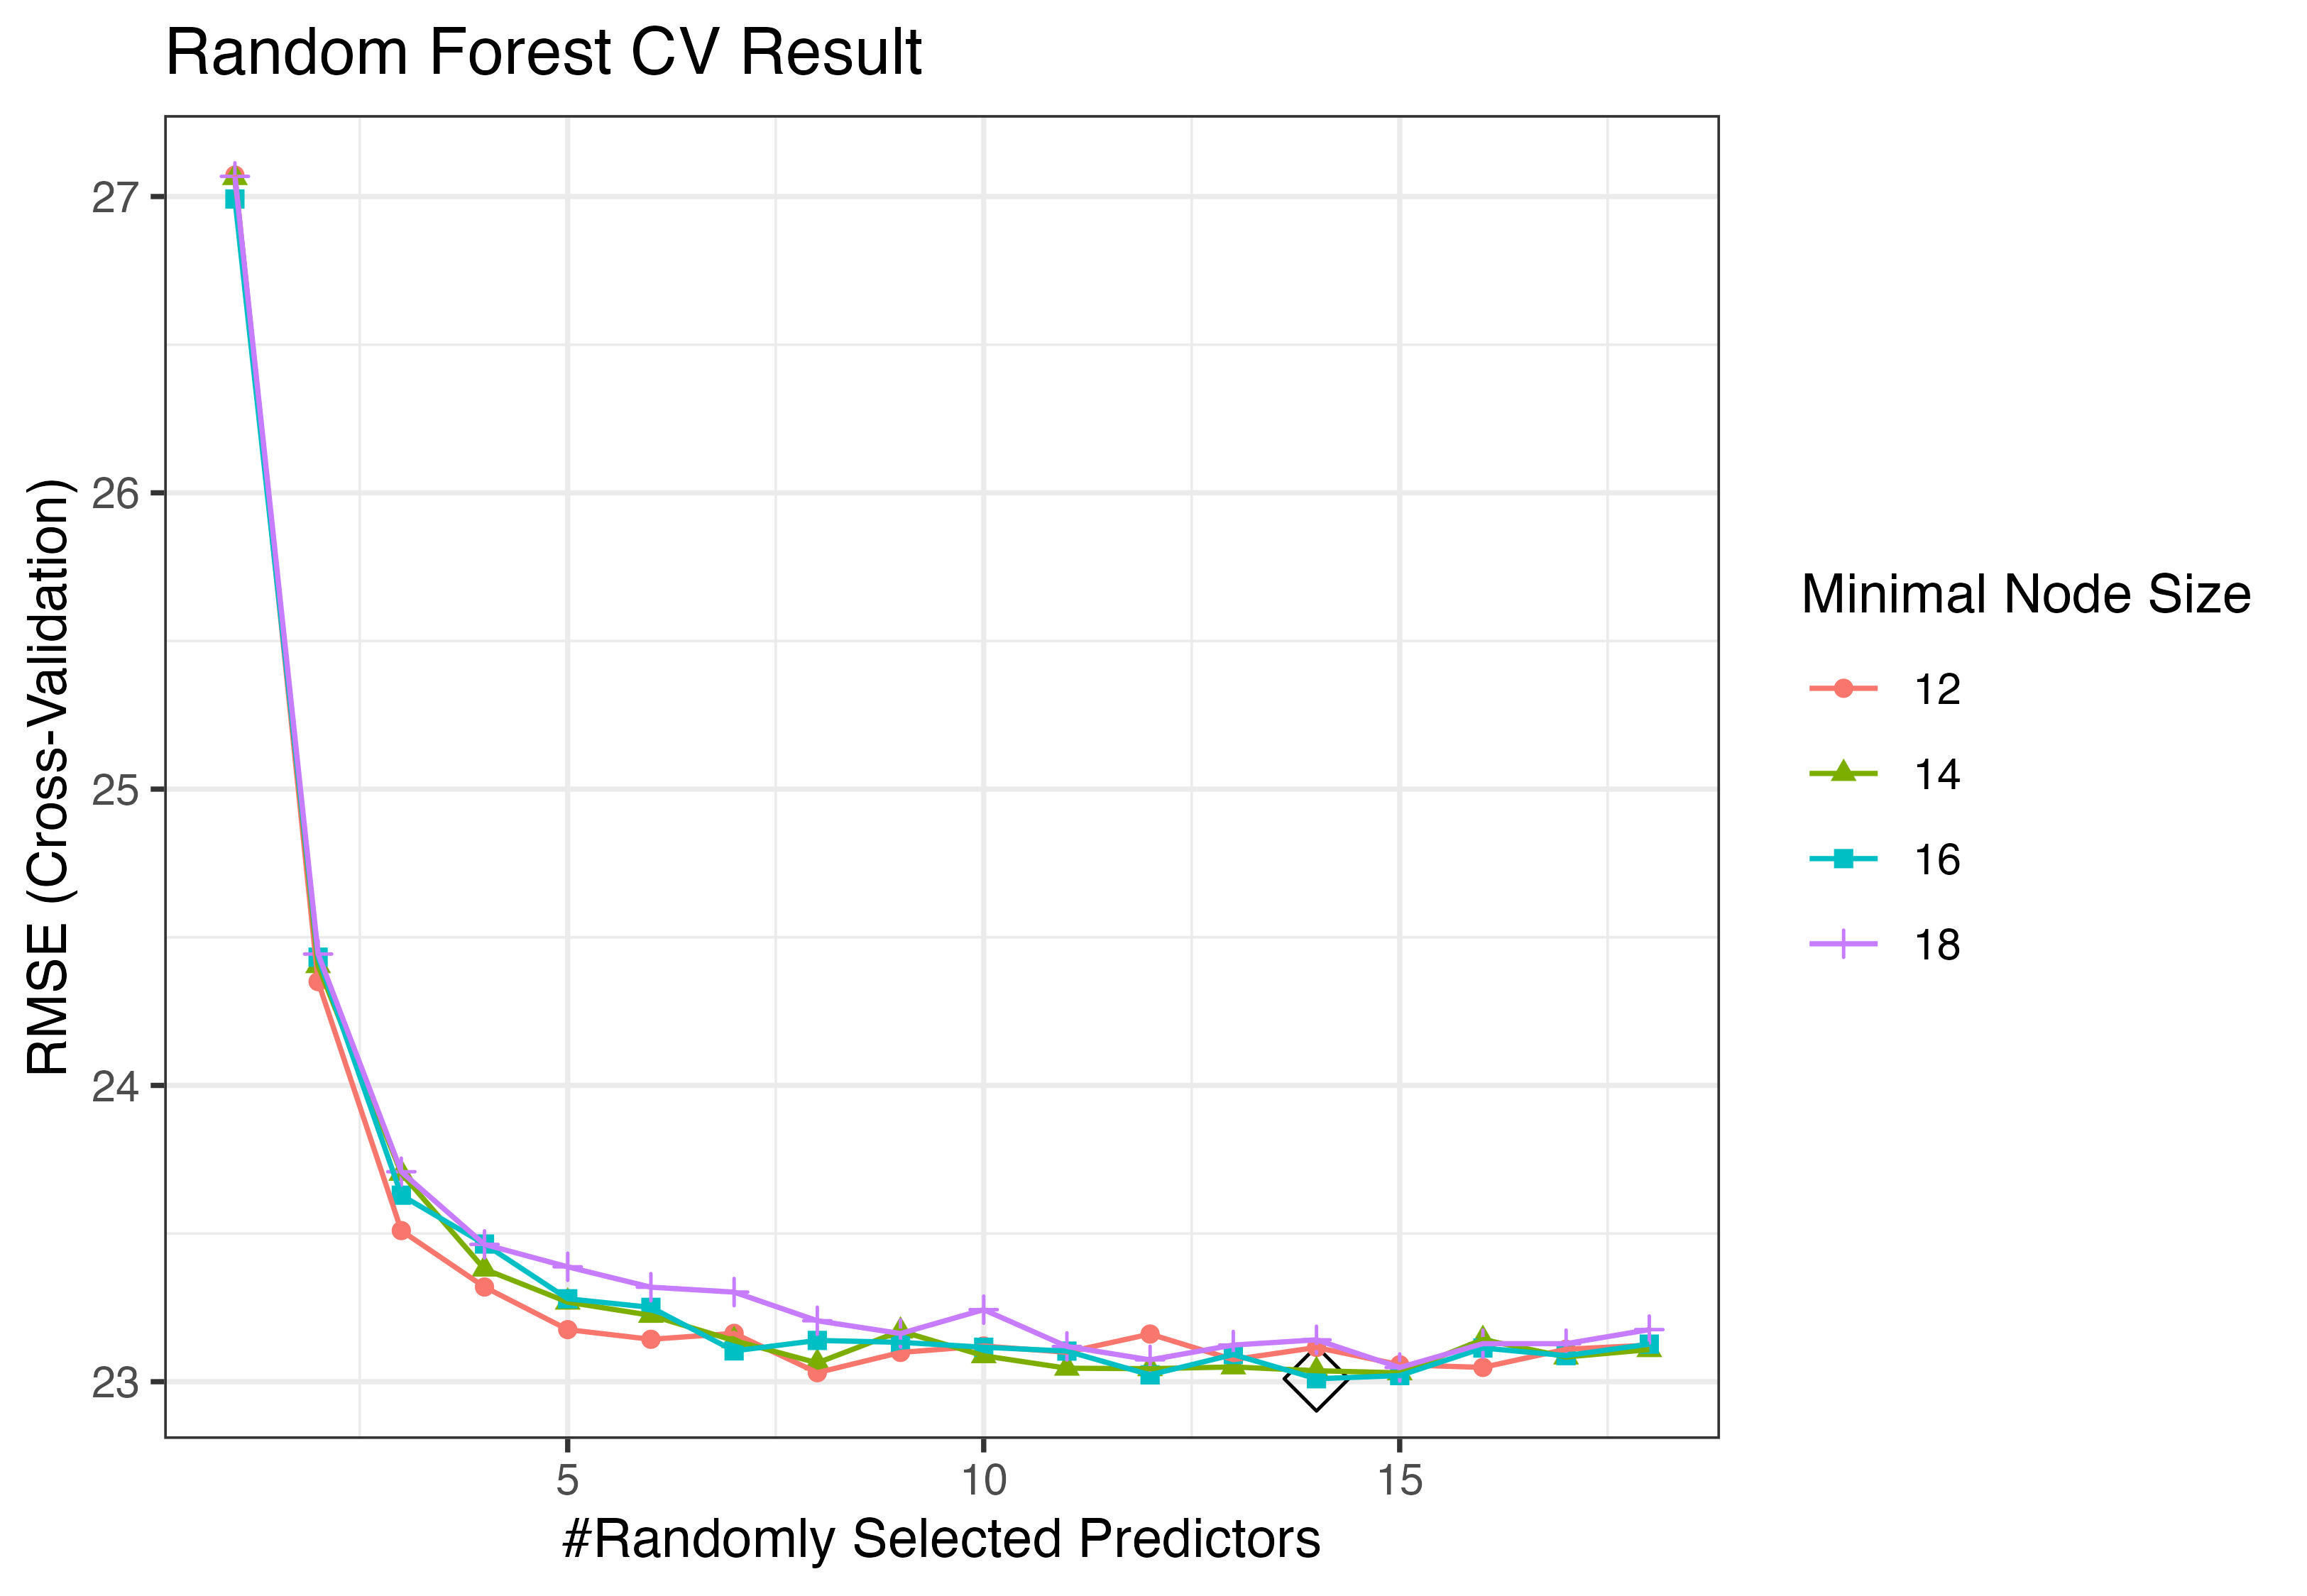
\includegraphics[width=0.32\textwidth]{primary/rf_cv.jpeg}\label{fig:rf}}
    \hspace{0.1cm}
    % 2
    \subfigure[Boosting]{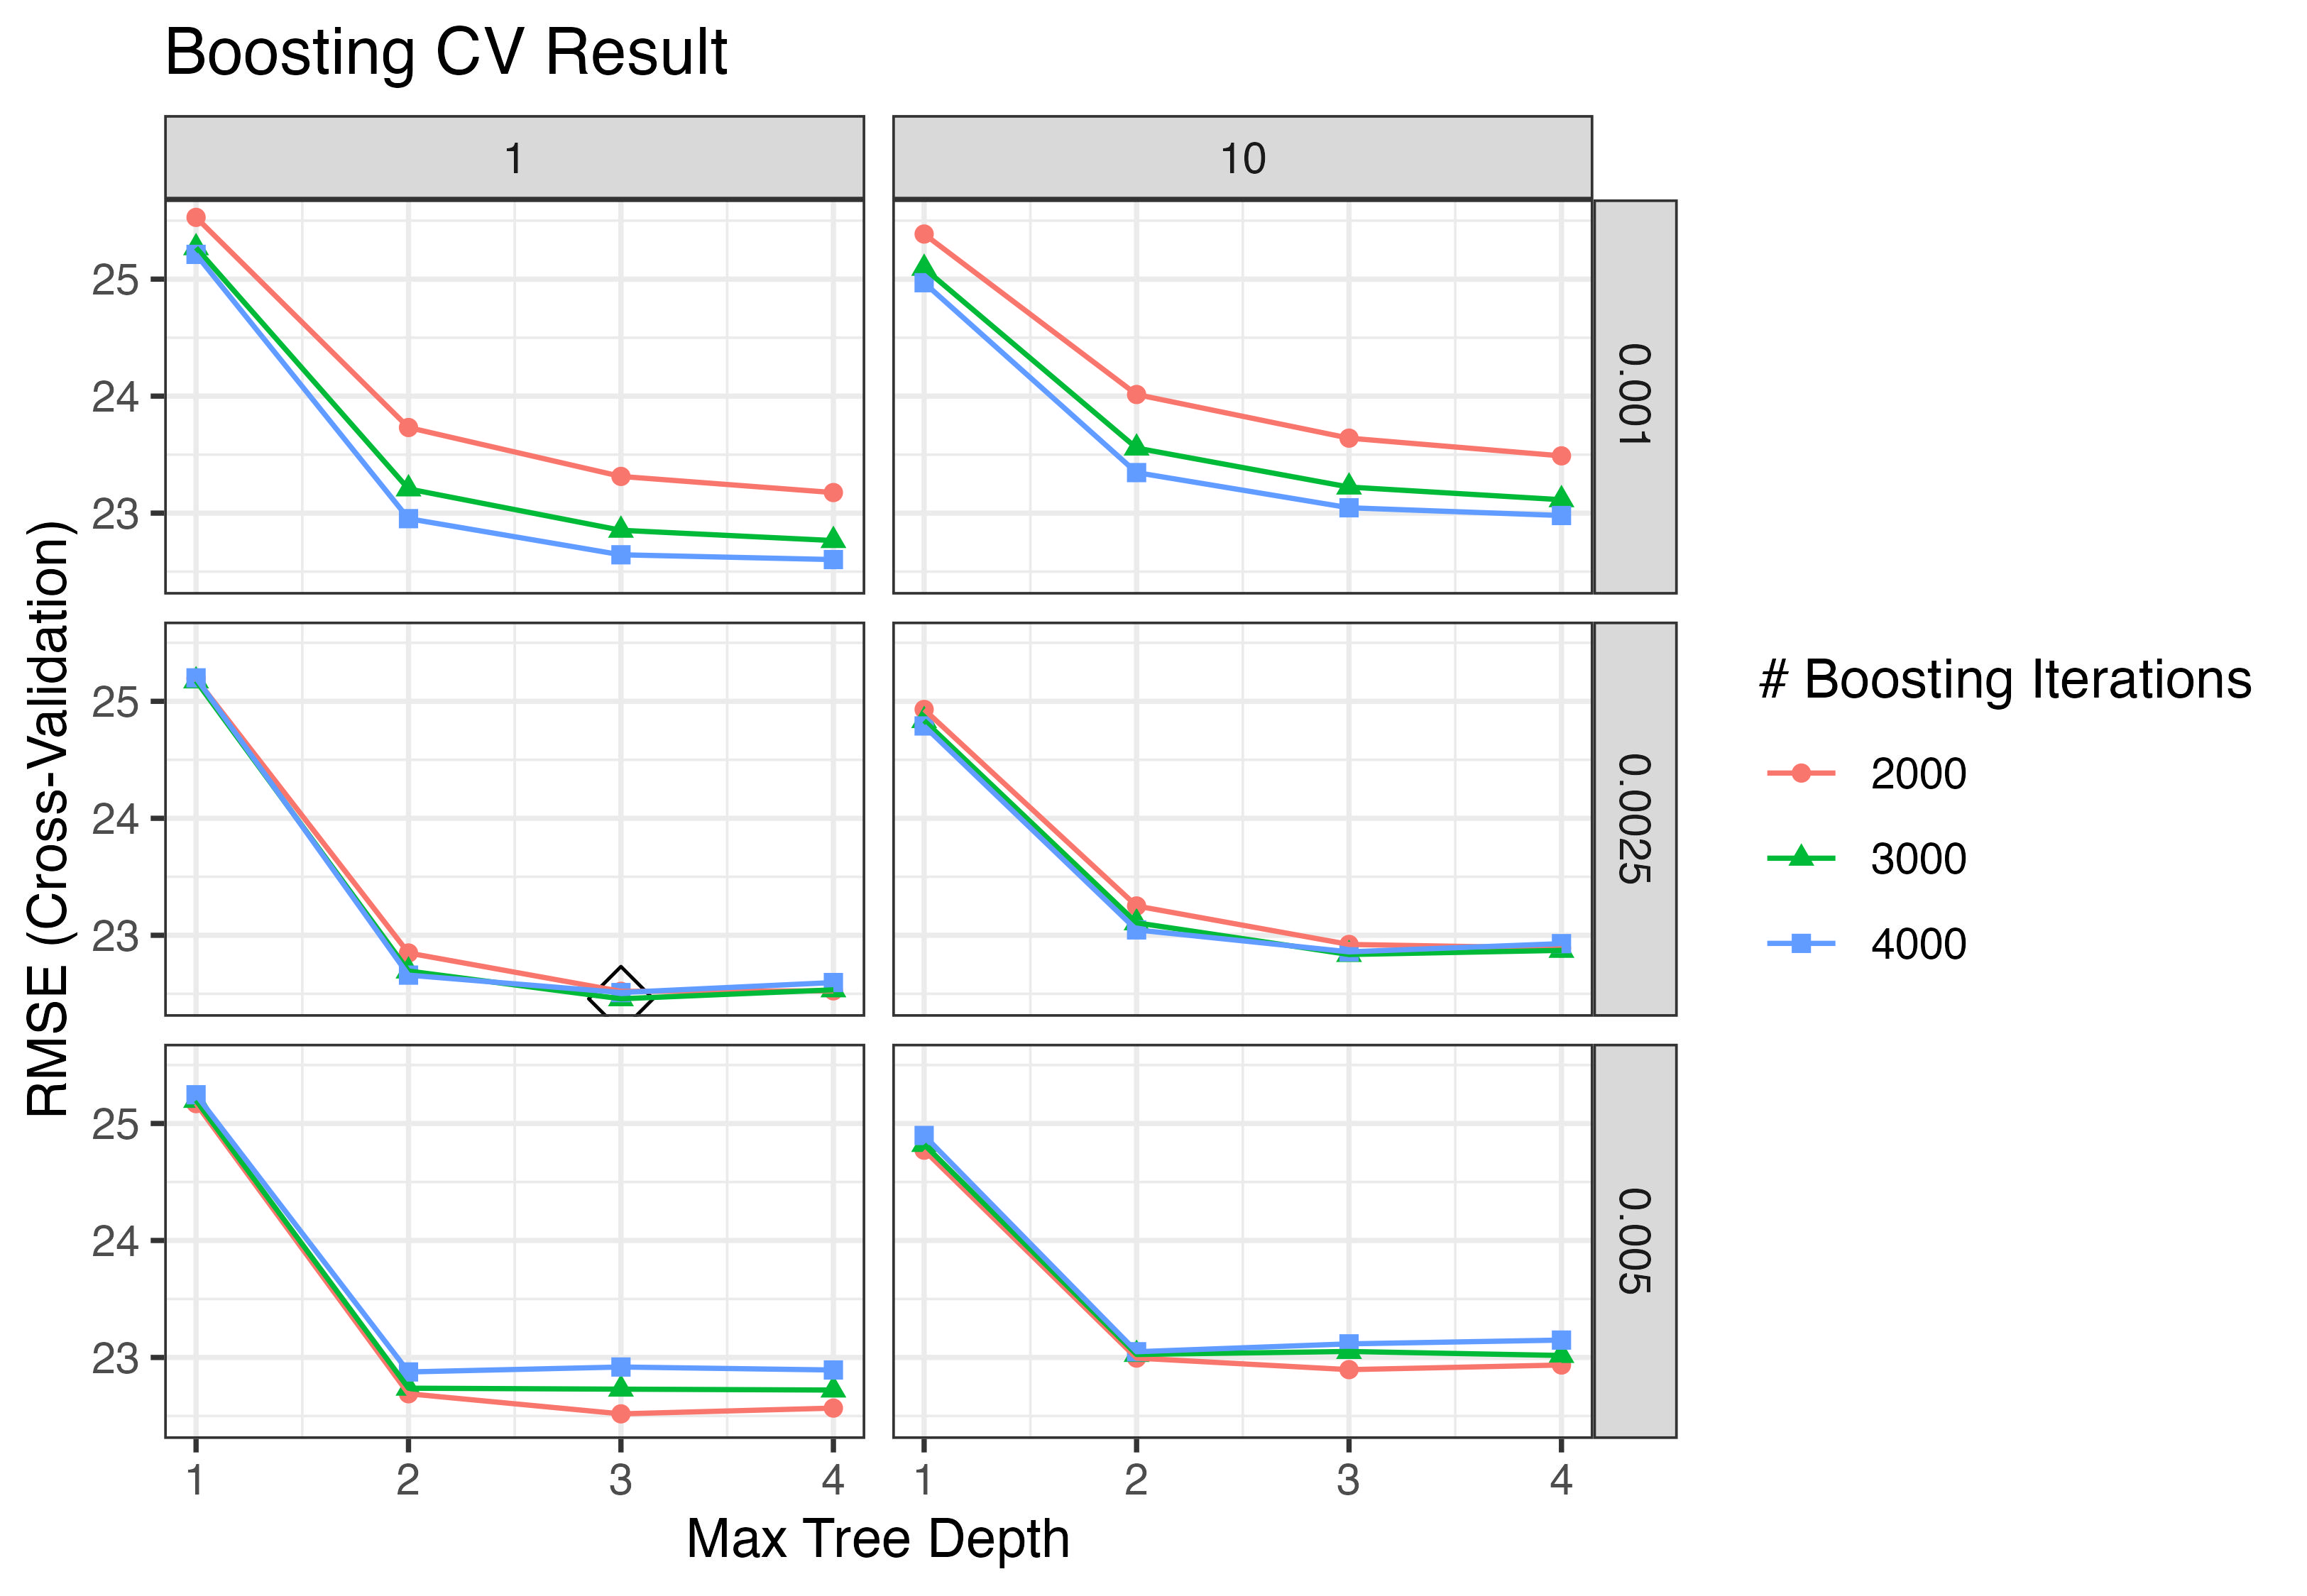
\includegraphics[width=0.32\textwidth]{primary/boosting_cv.jpeg}\label{fig:boosting}}
    \hspace{0.1cm}
    % 3
    \subfigure[Regression tree]{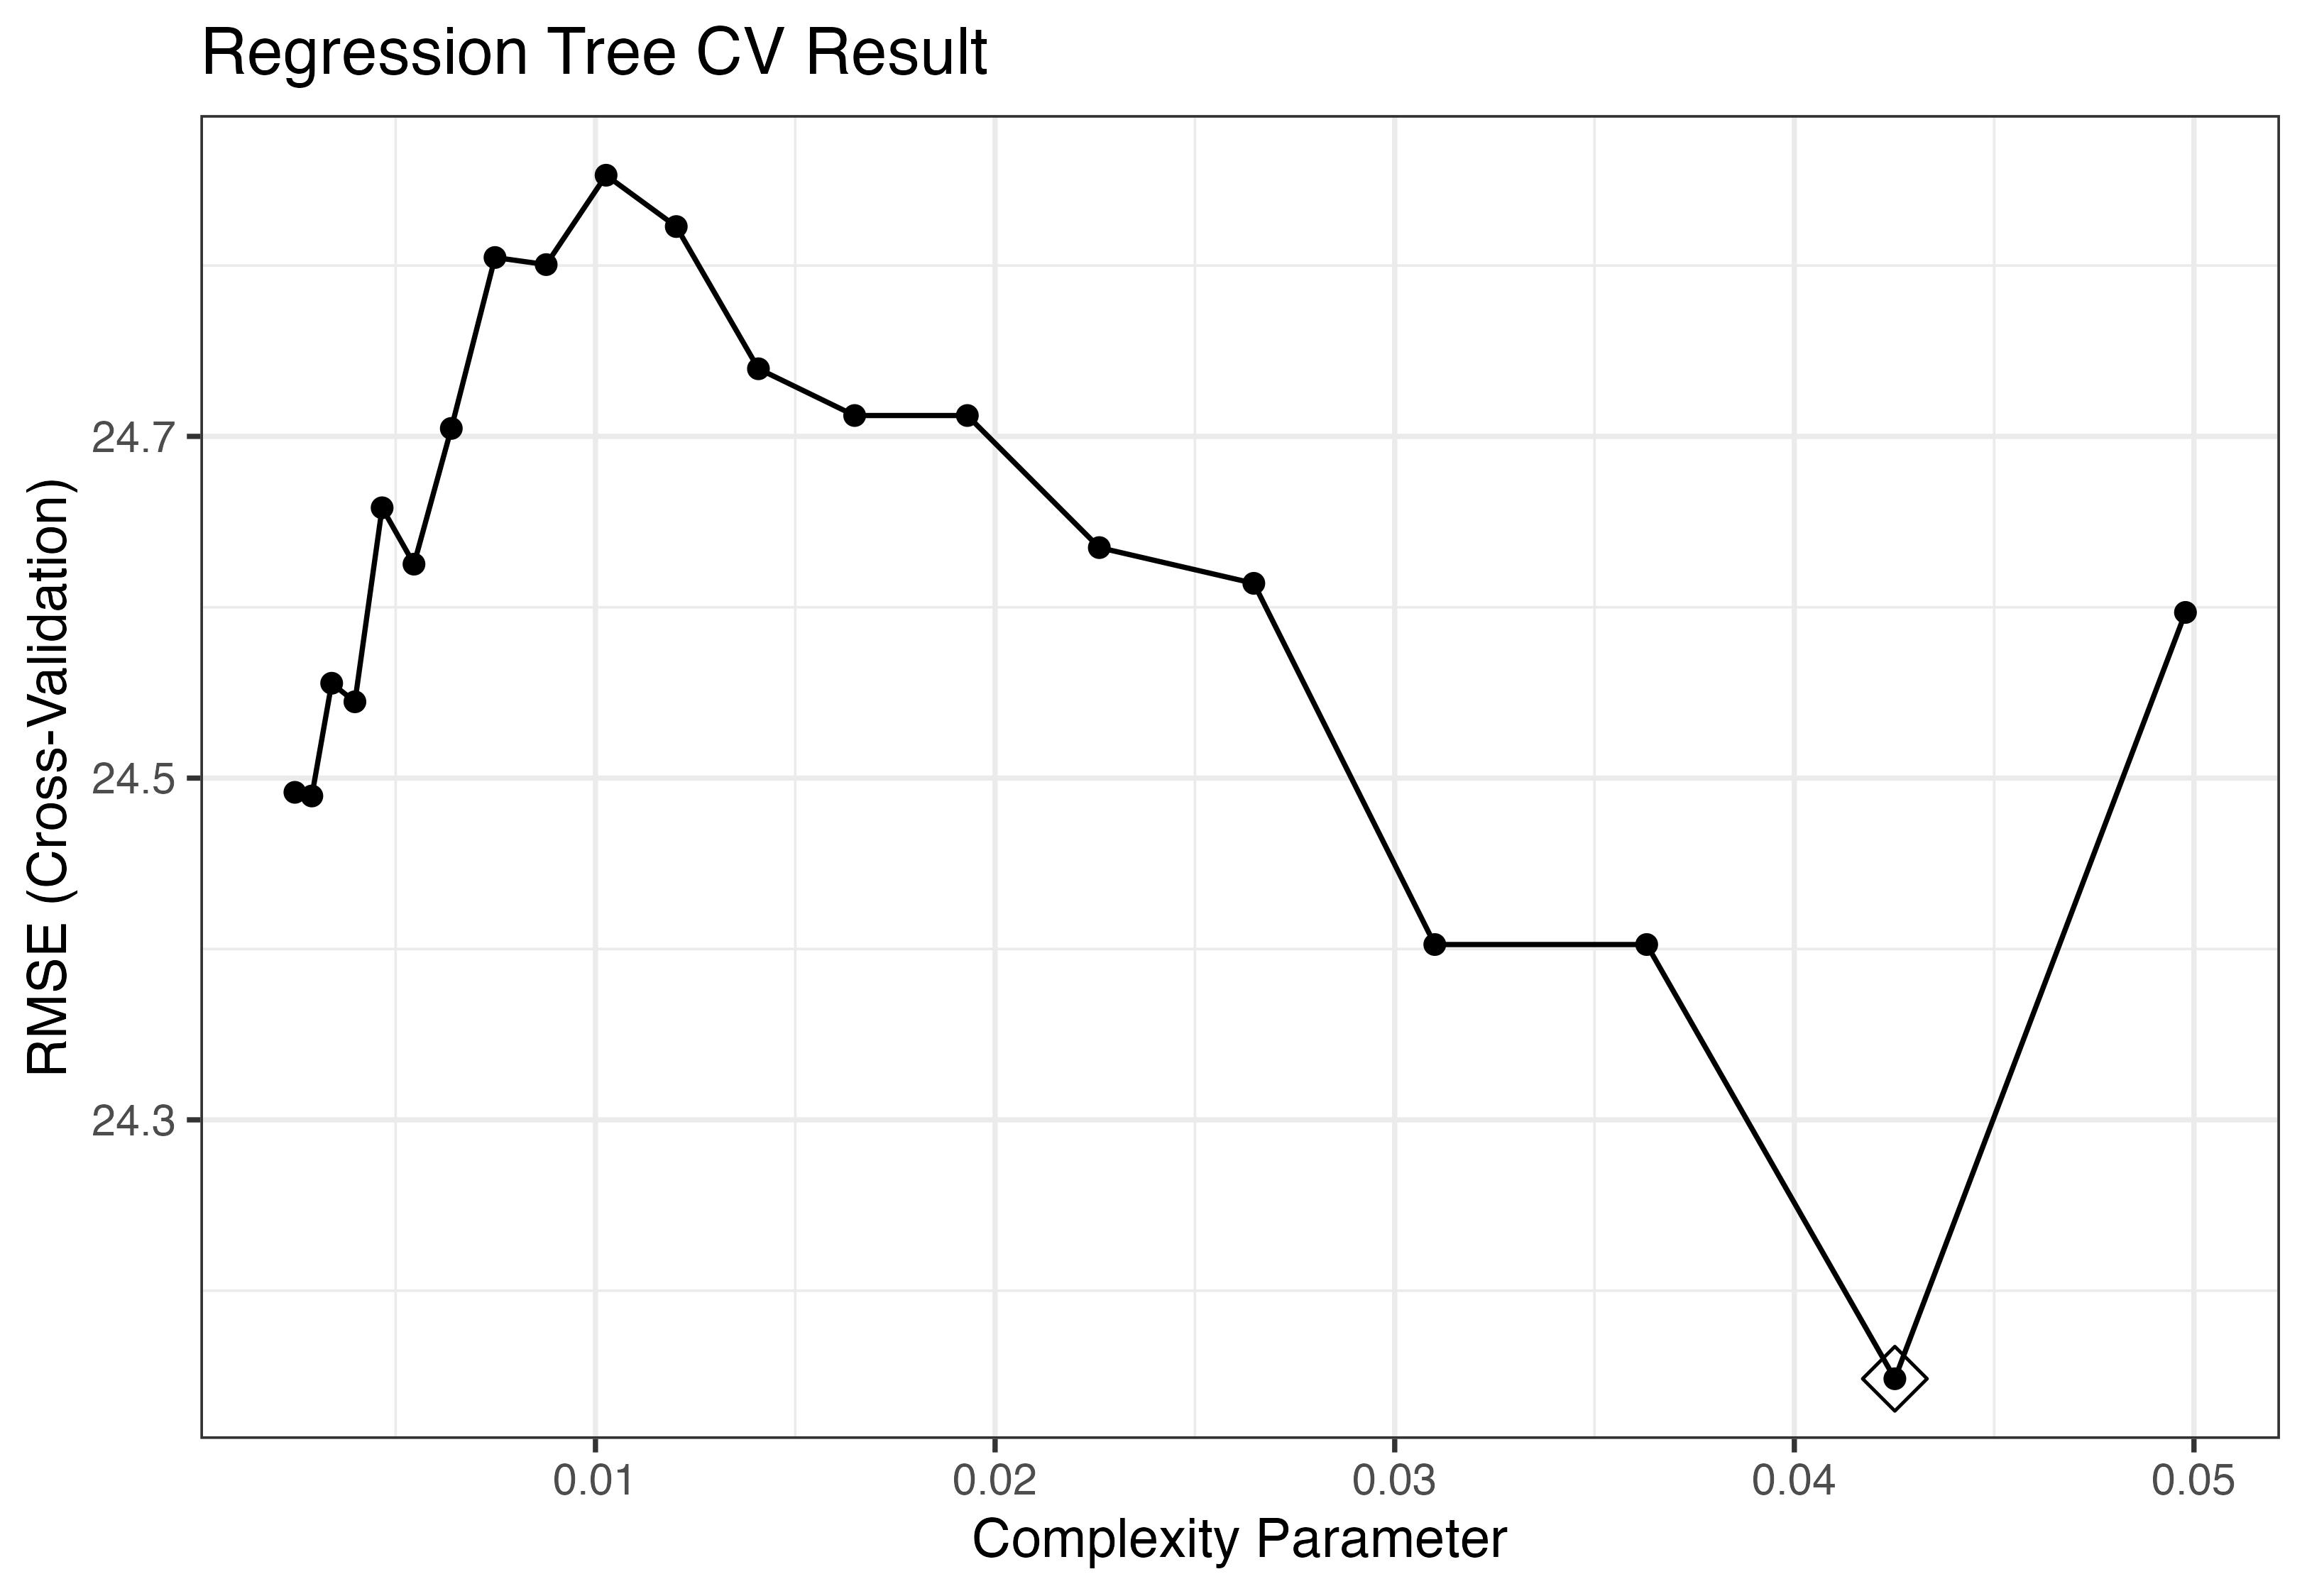
\includegraphics[width=0.32\textwidth]{primary/rpart1_cv.jpeg}\label{fig:regtree}}
    
    \caption{Primary analysis CV results}
    \label{fig:primary}
\end{figure}


\begin{figure}
    \centering
    % 1
    \subfigure[Penalized logistic regression]{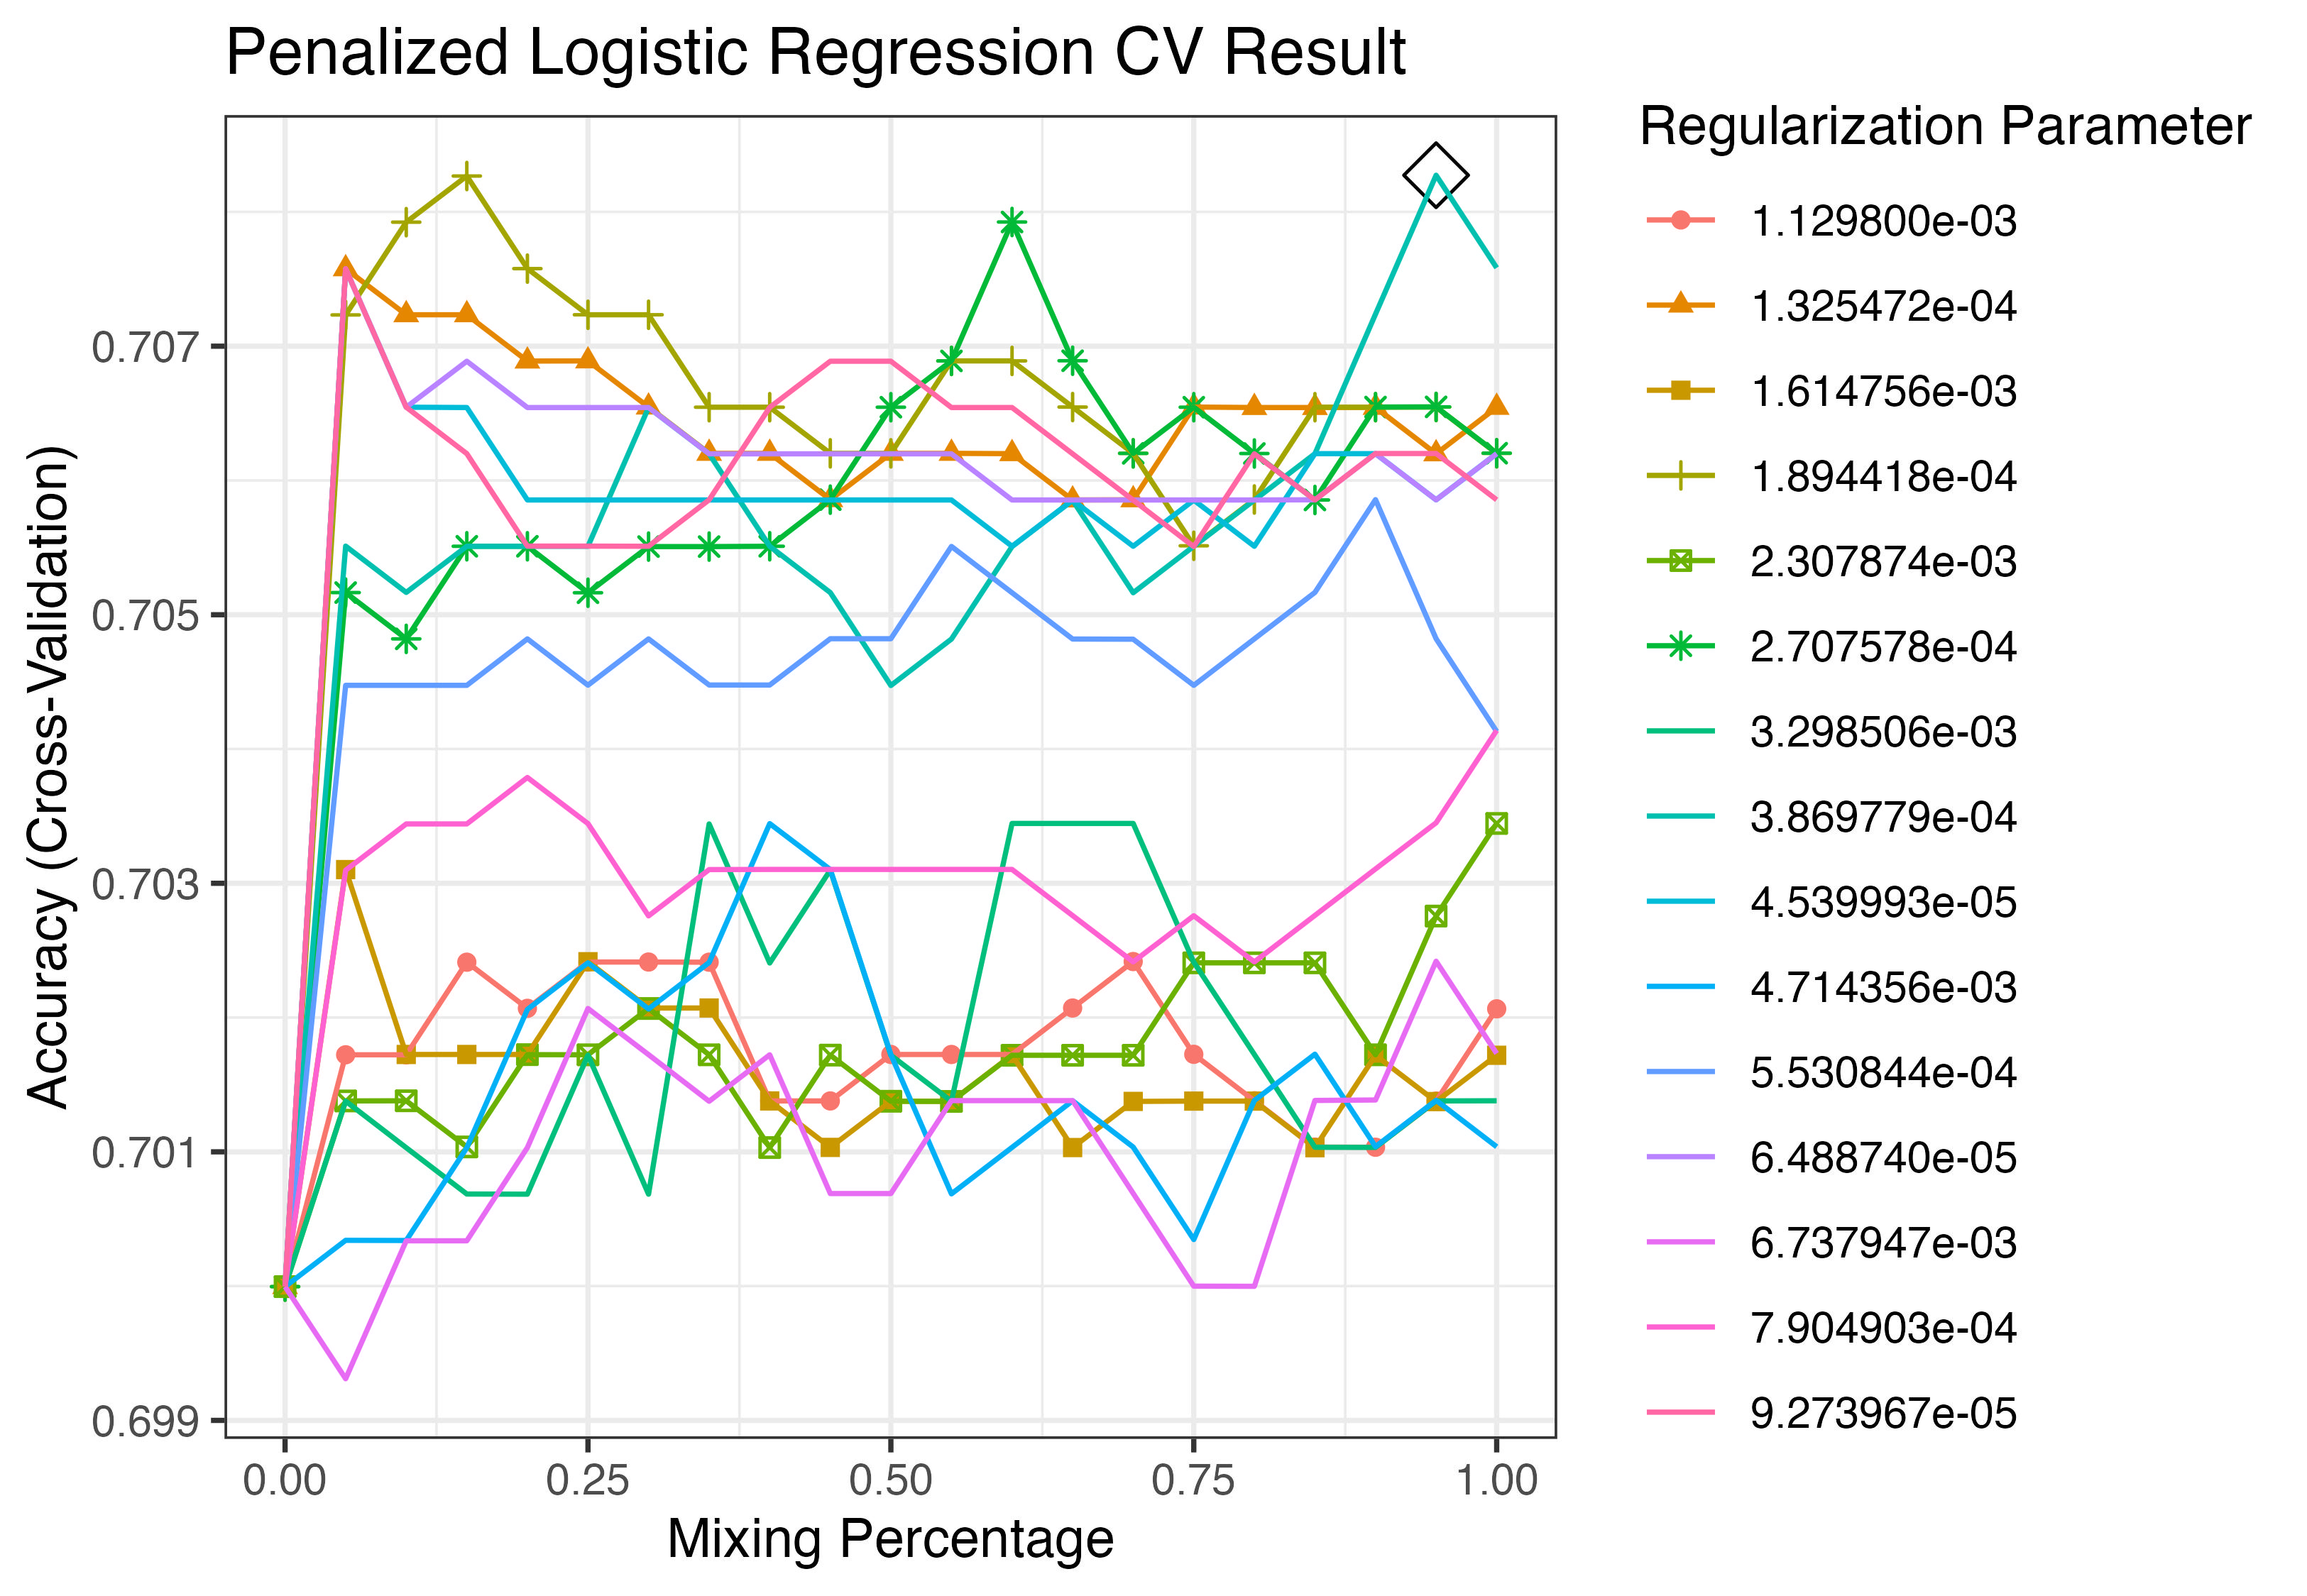
\includegraphics[width=0.32\textwidth]{secondary/penal_logi_cv.jpeg}\label{fig:plogi}}
    \hspace{0.1cm}
    % 2
    \subfigure[GAM]{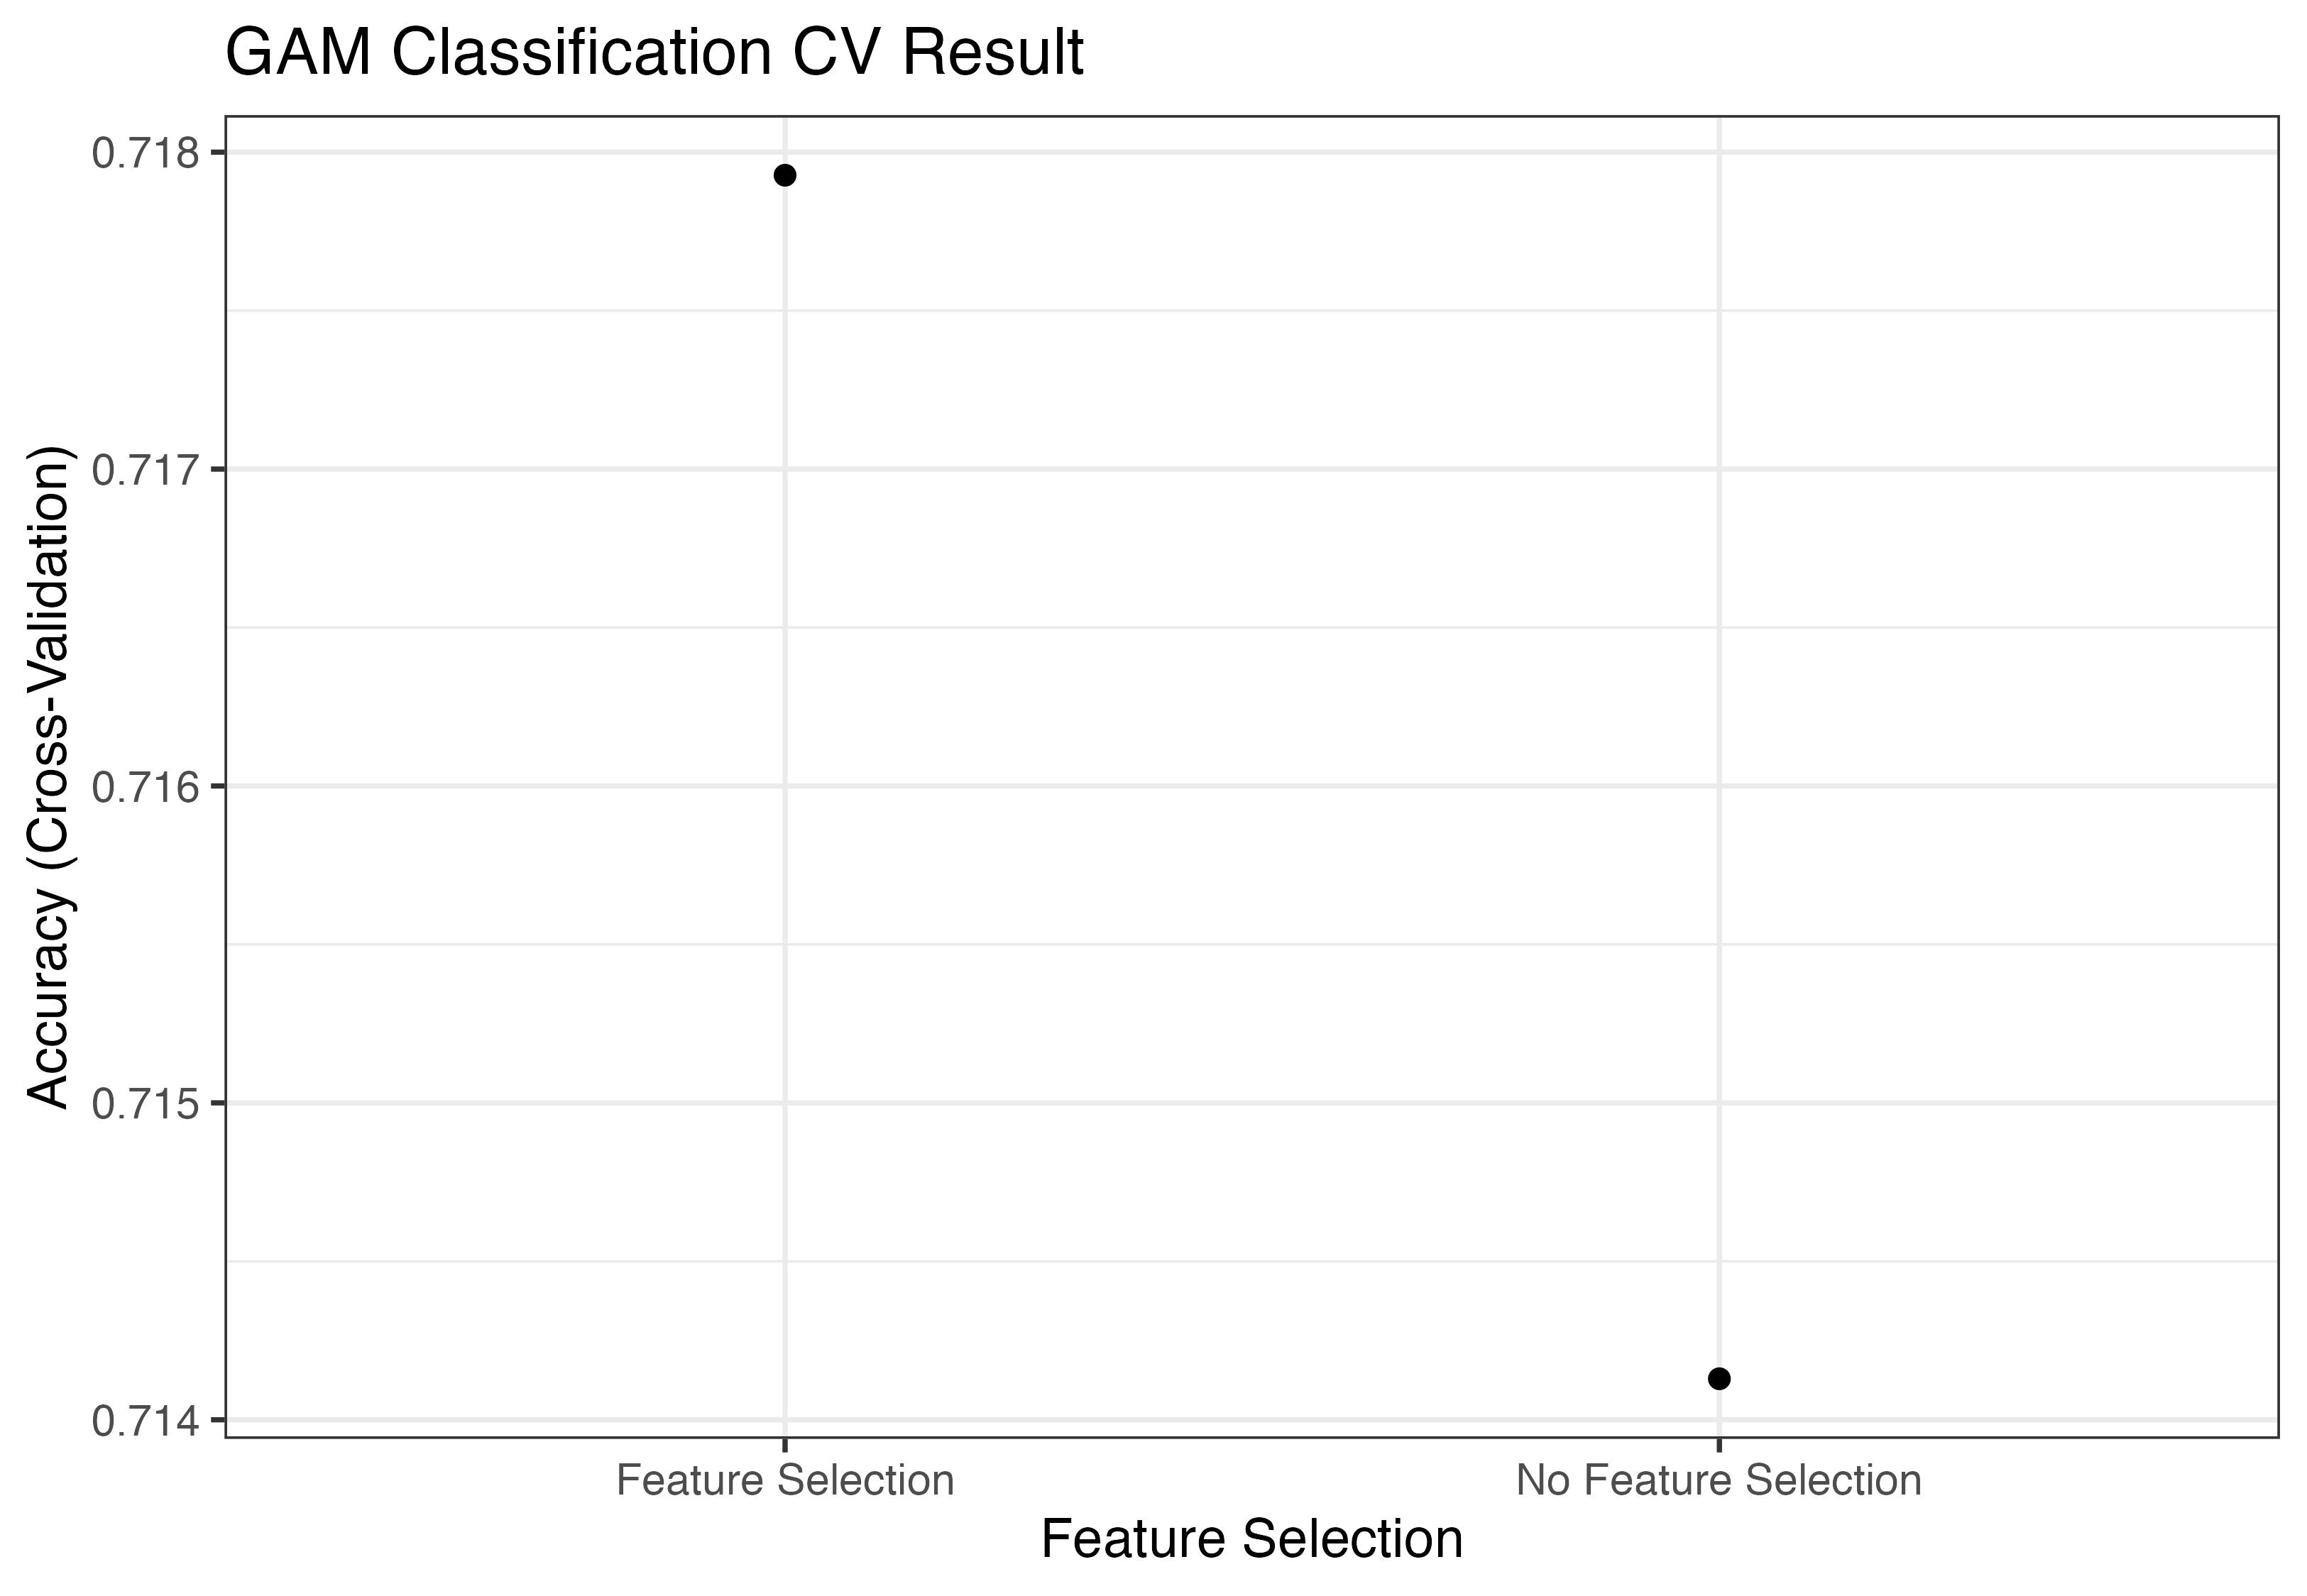
\includegraphics[width=0.32\textwidth]{secondary/gam_binned_cv.jpeg}\label{fig:gam_bin}}
    \hspace{0.1cm}
    % 3
    \subfigure[MARS]{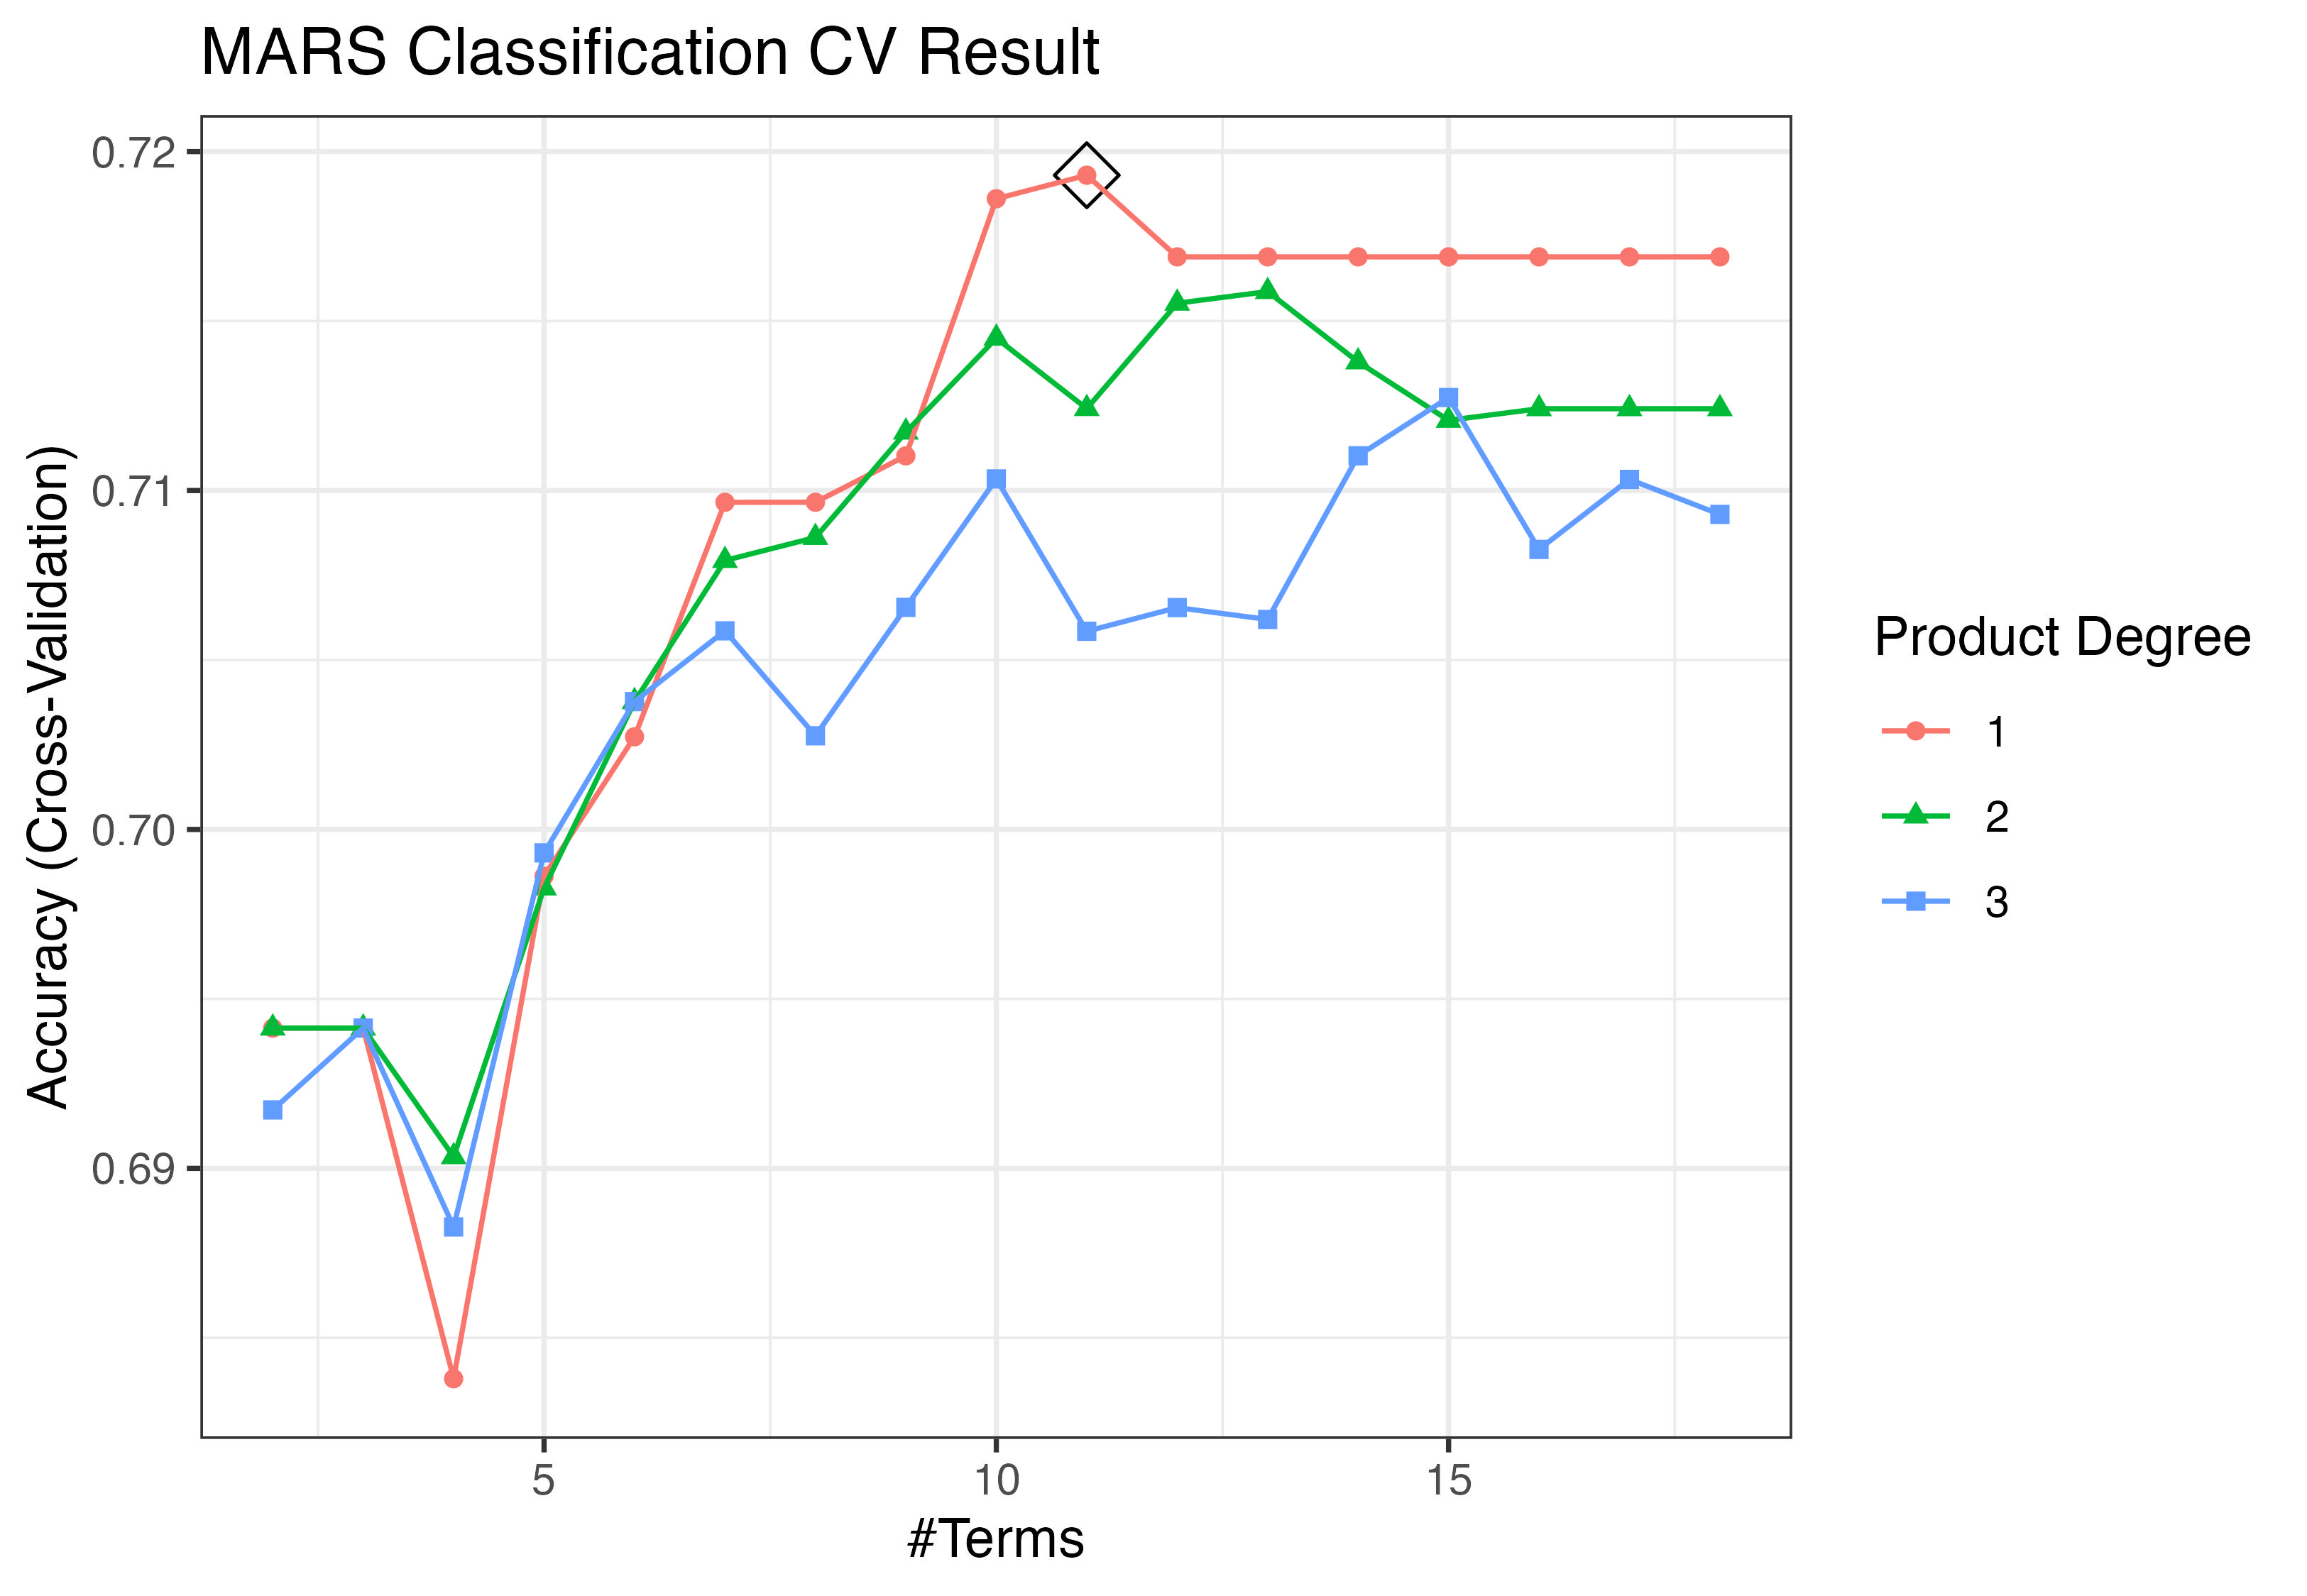
\includegraphics[width=0.32\textwidth]{secondary/mars_binned_cv.jpeg}\label{fig:mars_bin}}

    % 1
    \subfigure[Naive Bayes]{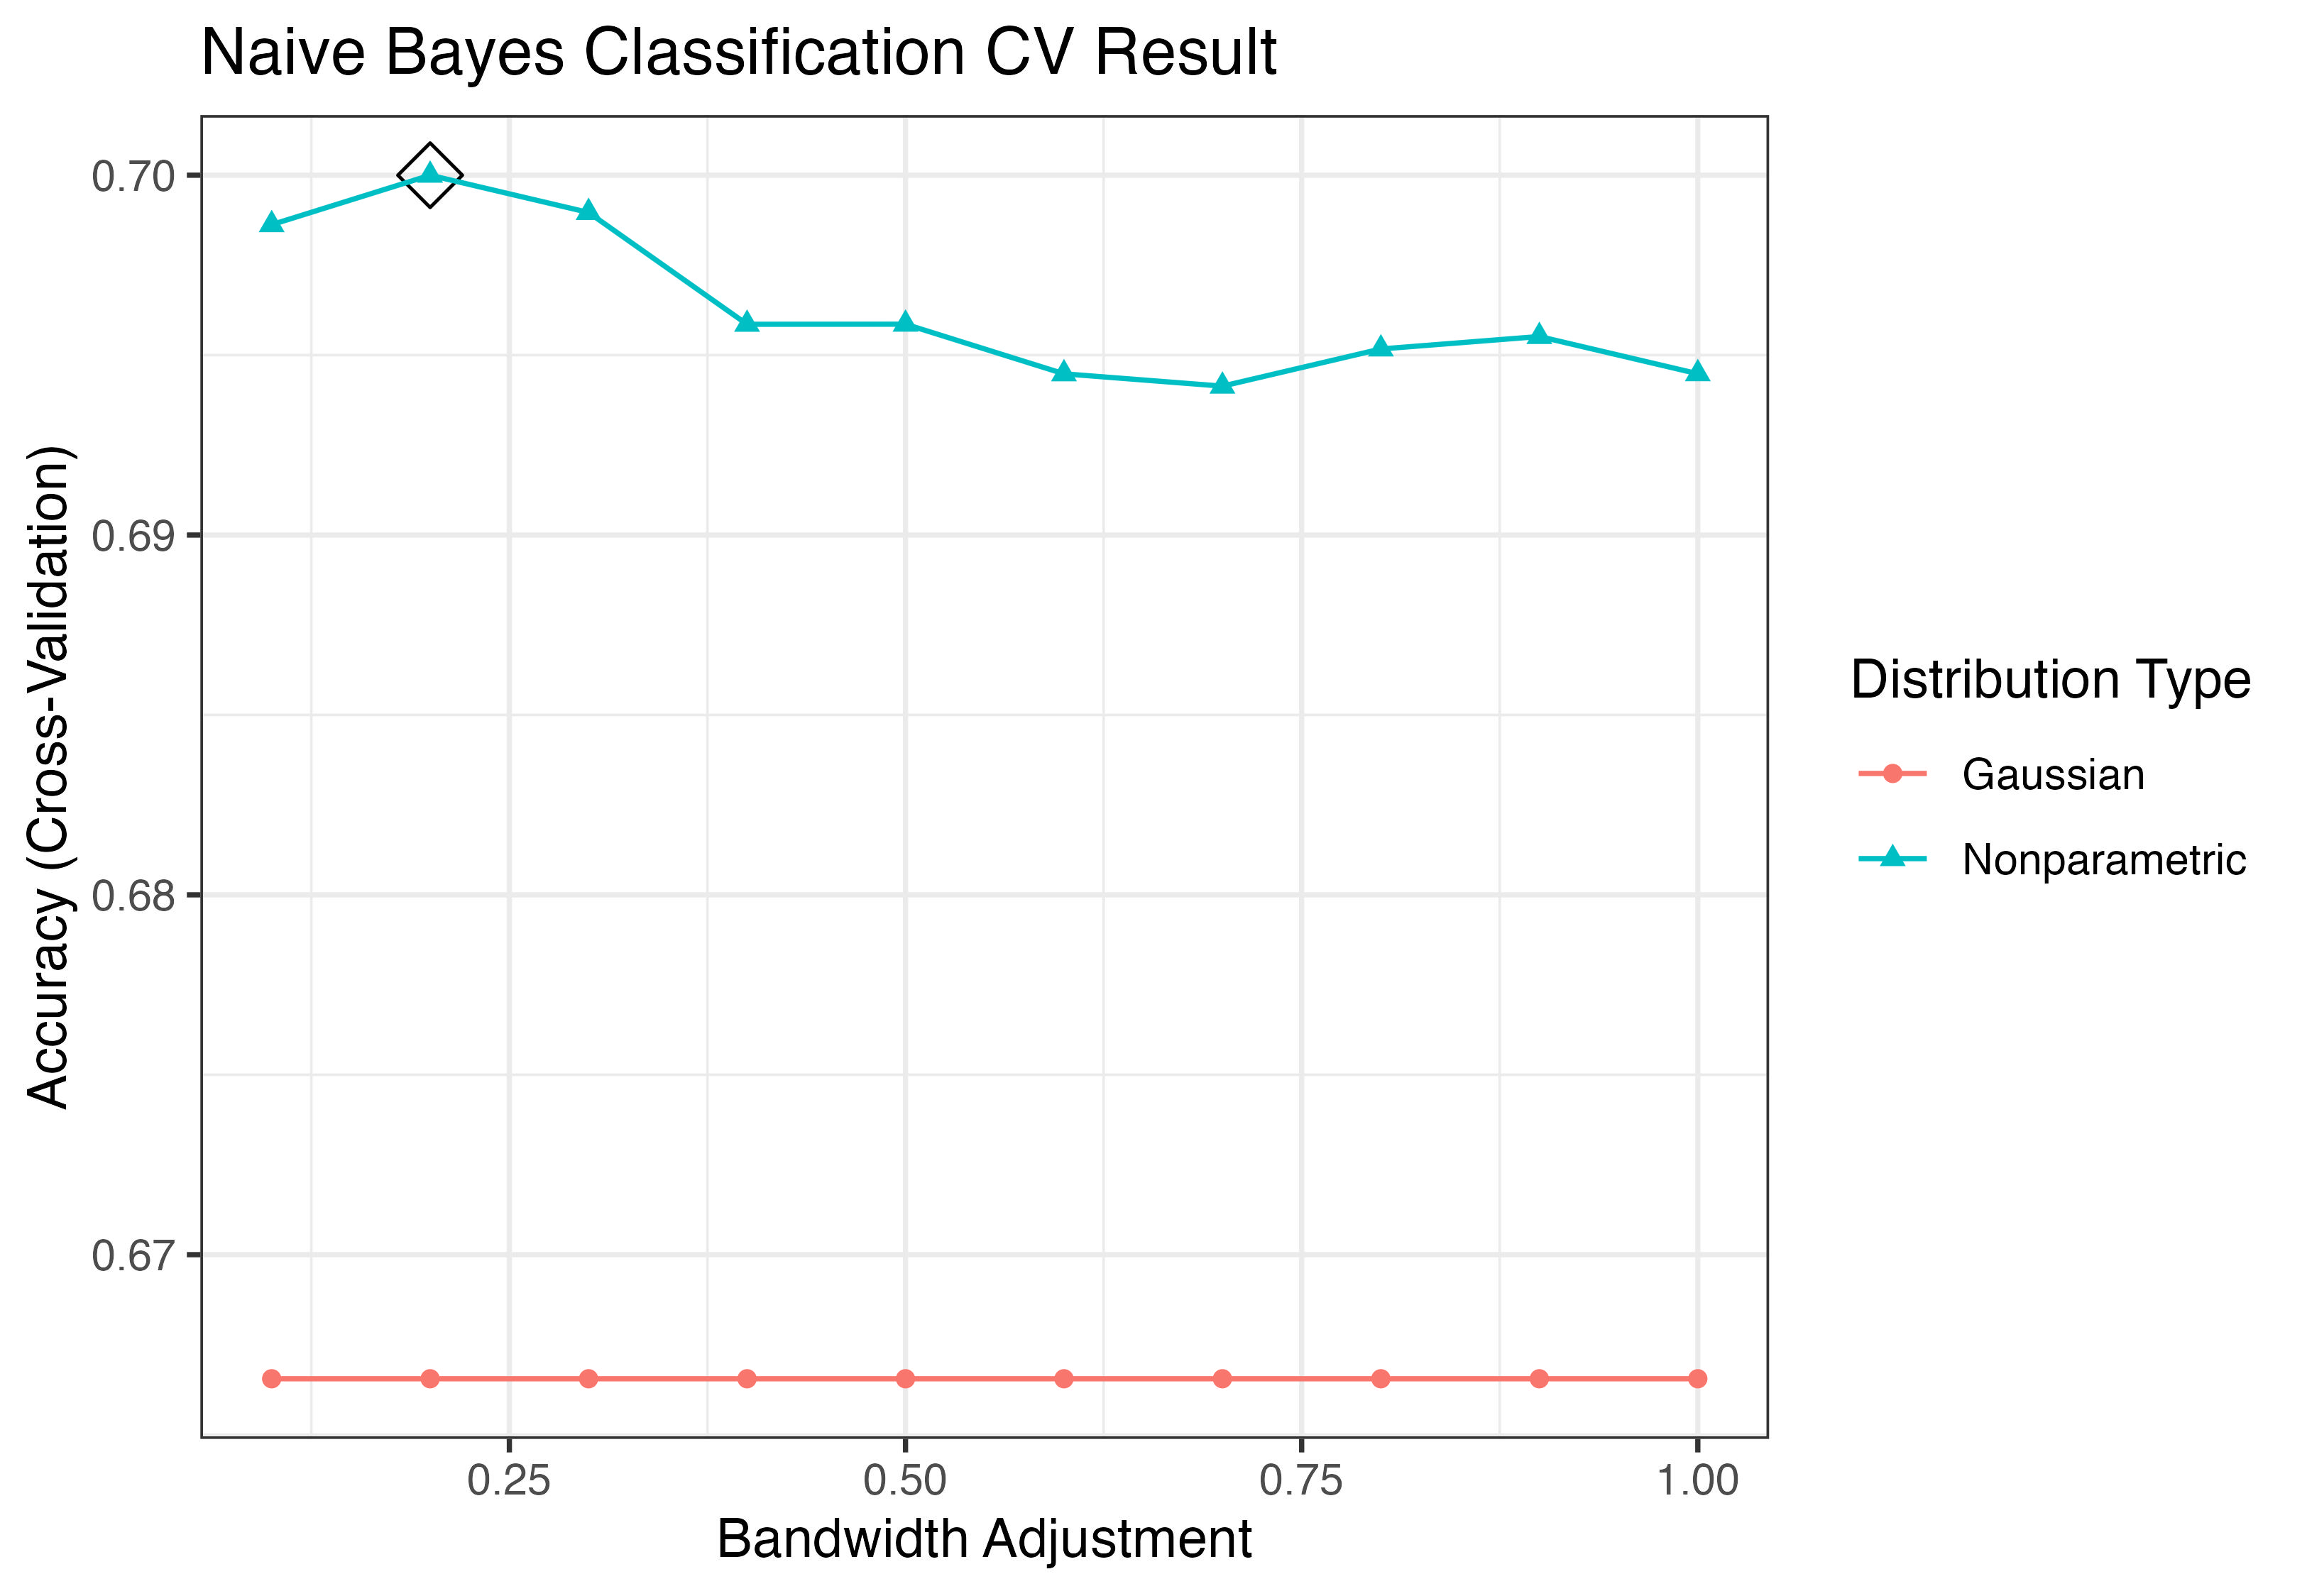
\includegraphics[width=0.32\textwidth]{secondary/nb_cv.jpeg}\label{fig:nb}}
    \hspace{0.1cm}
    % 2
    \subfigure[Bagging]{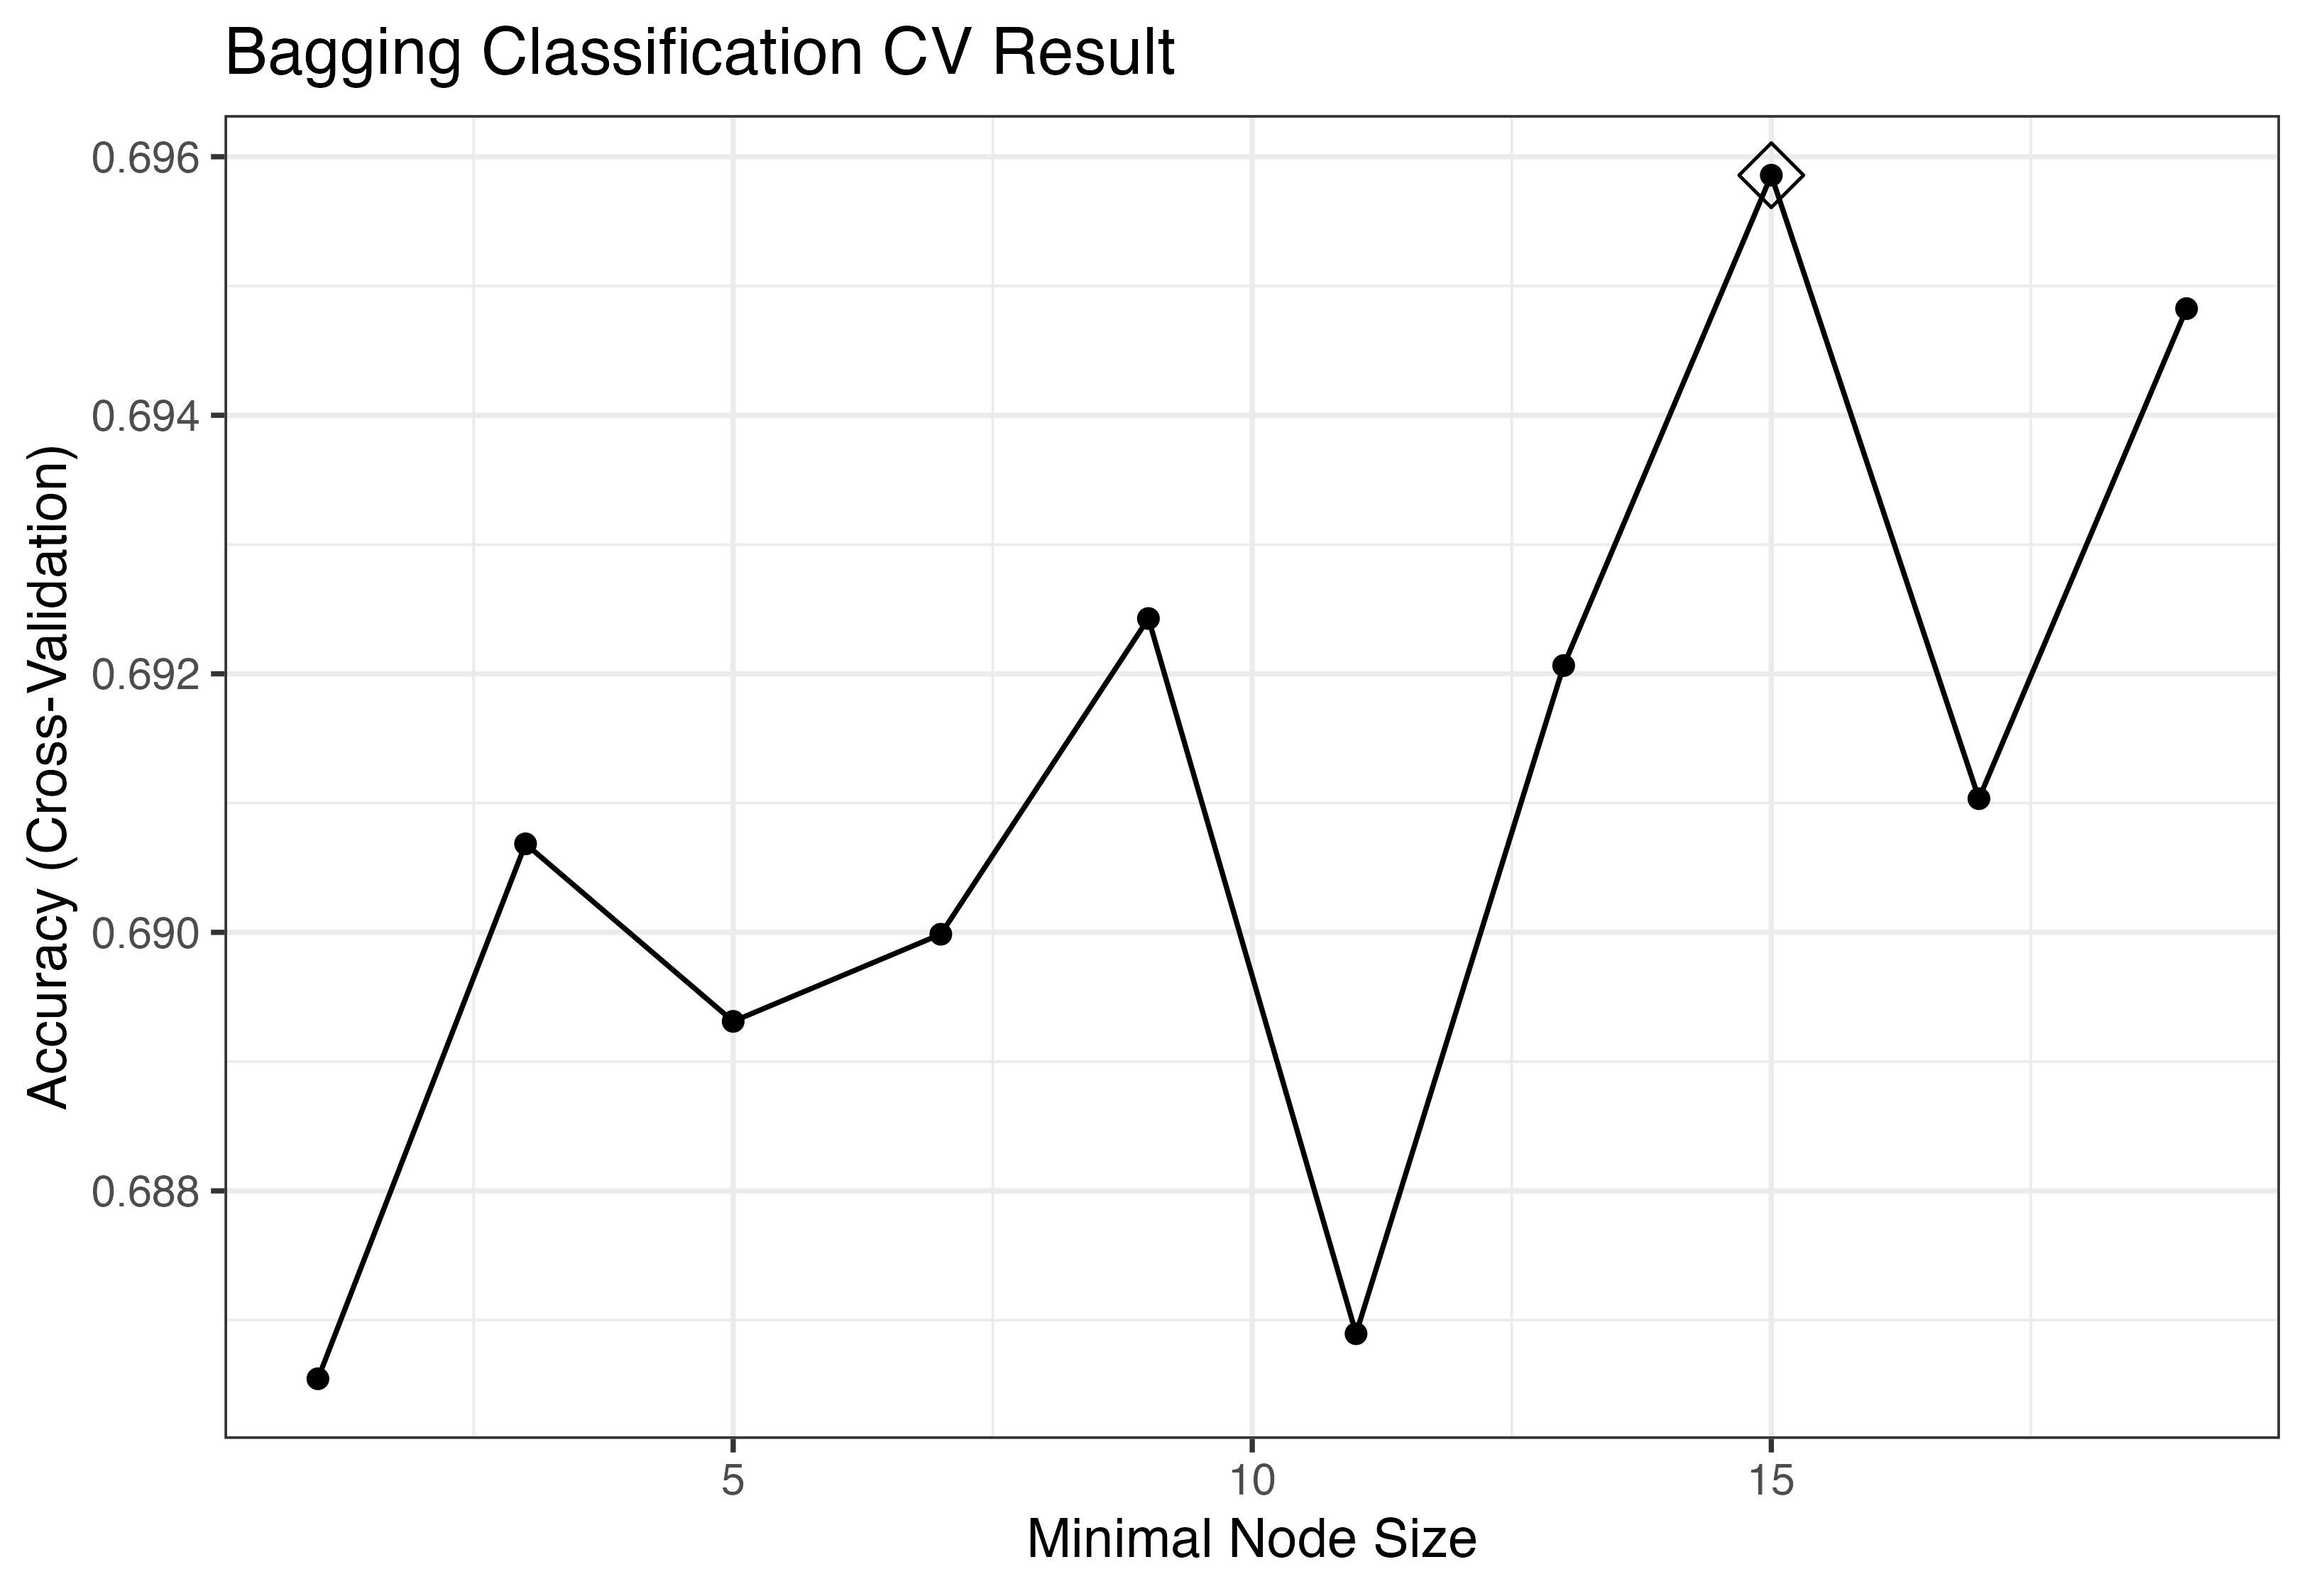
\includegraphics[width=0.32\textwidth]{secondary/bagging_classification_cv.jpeg}\label{fig:bagging_bin}}
    \hspace{0.1cm}
    % 3
    \subfigure[Random forest]{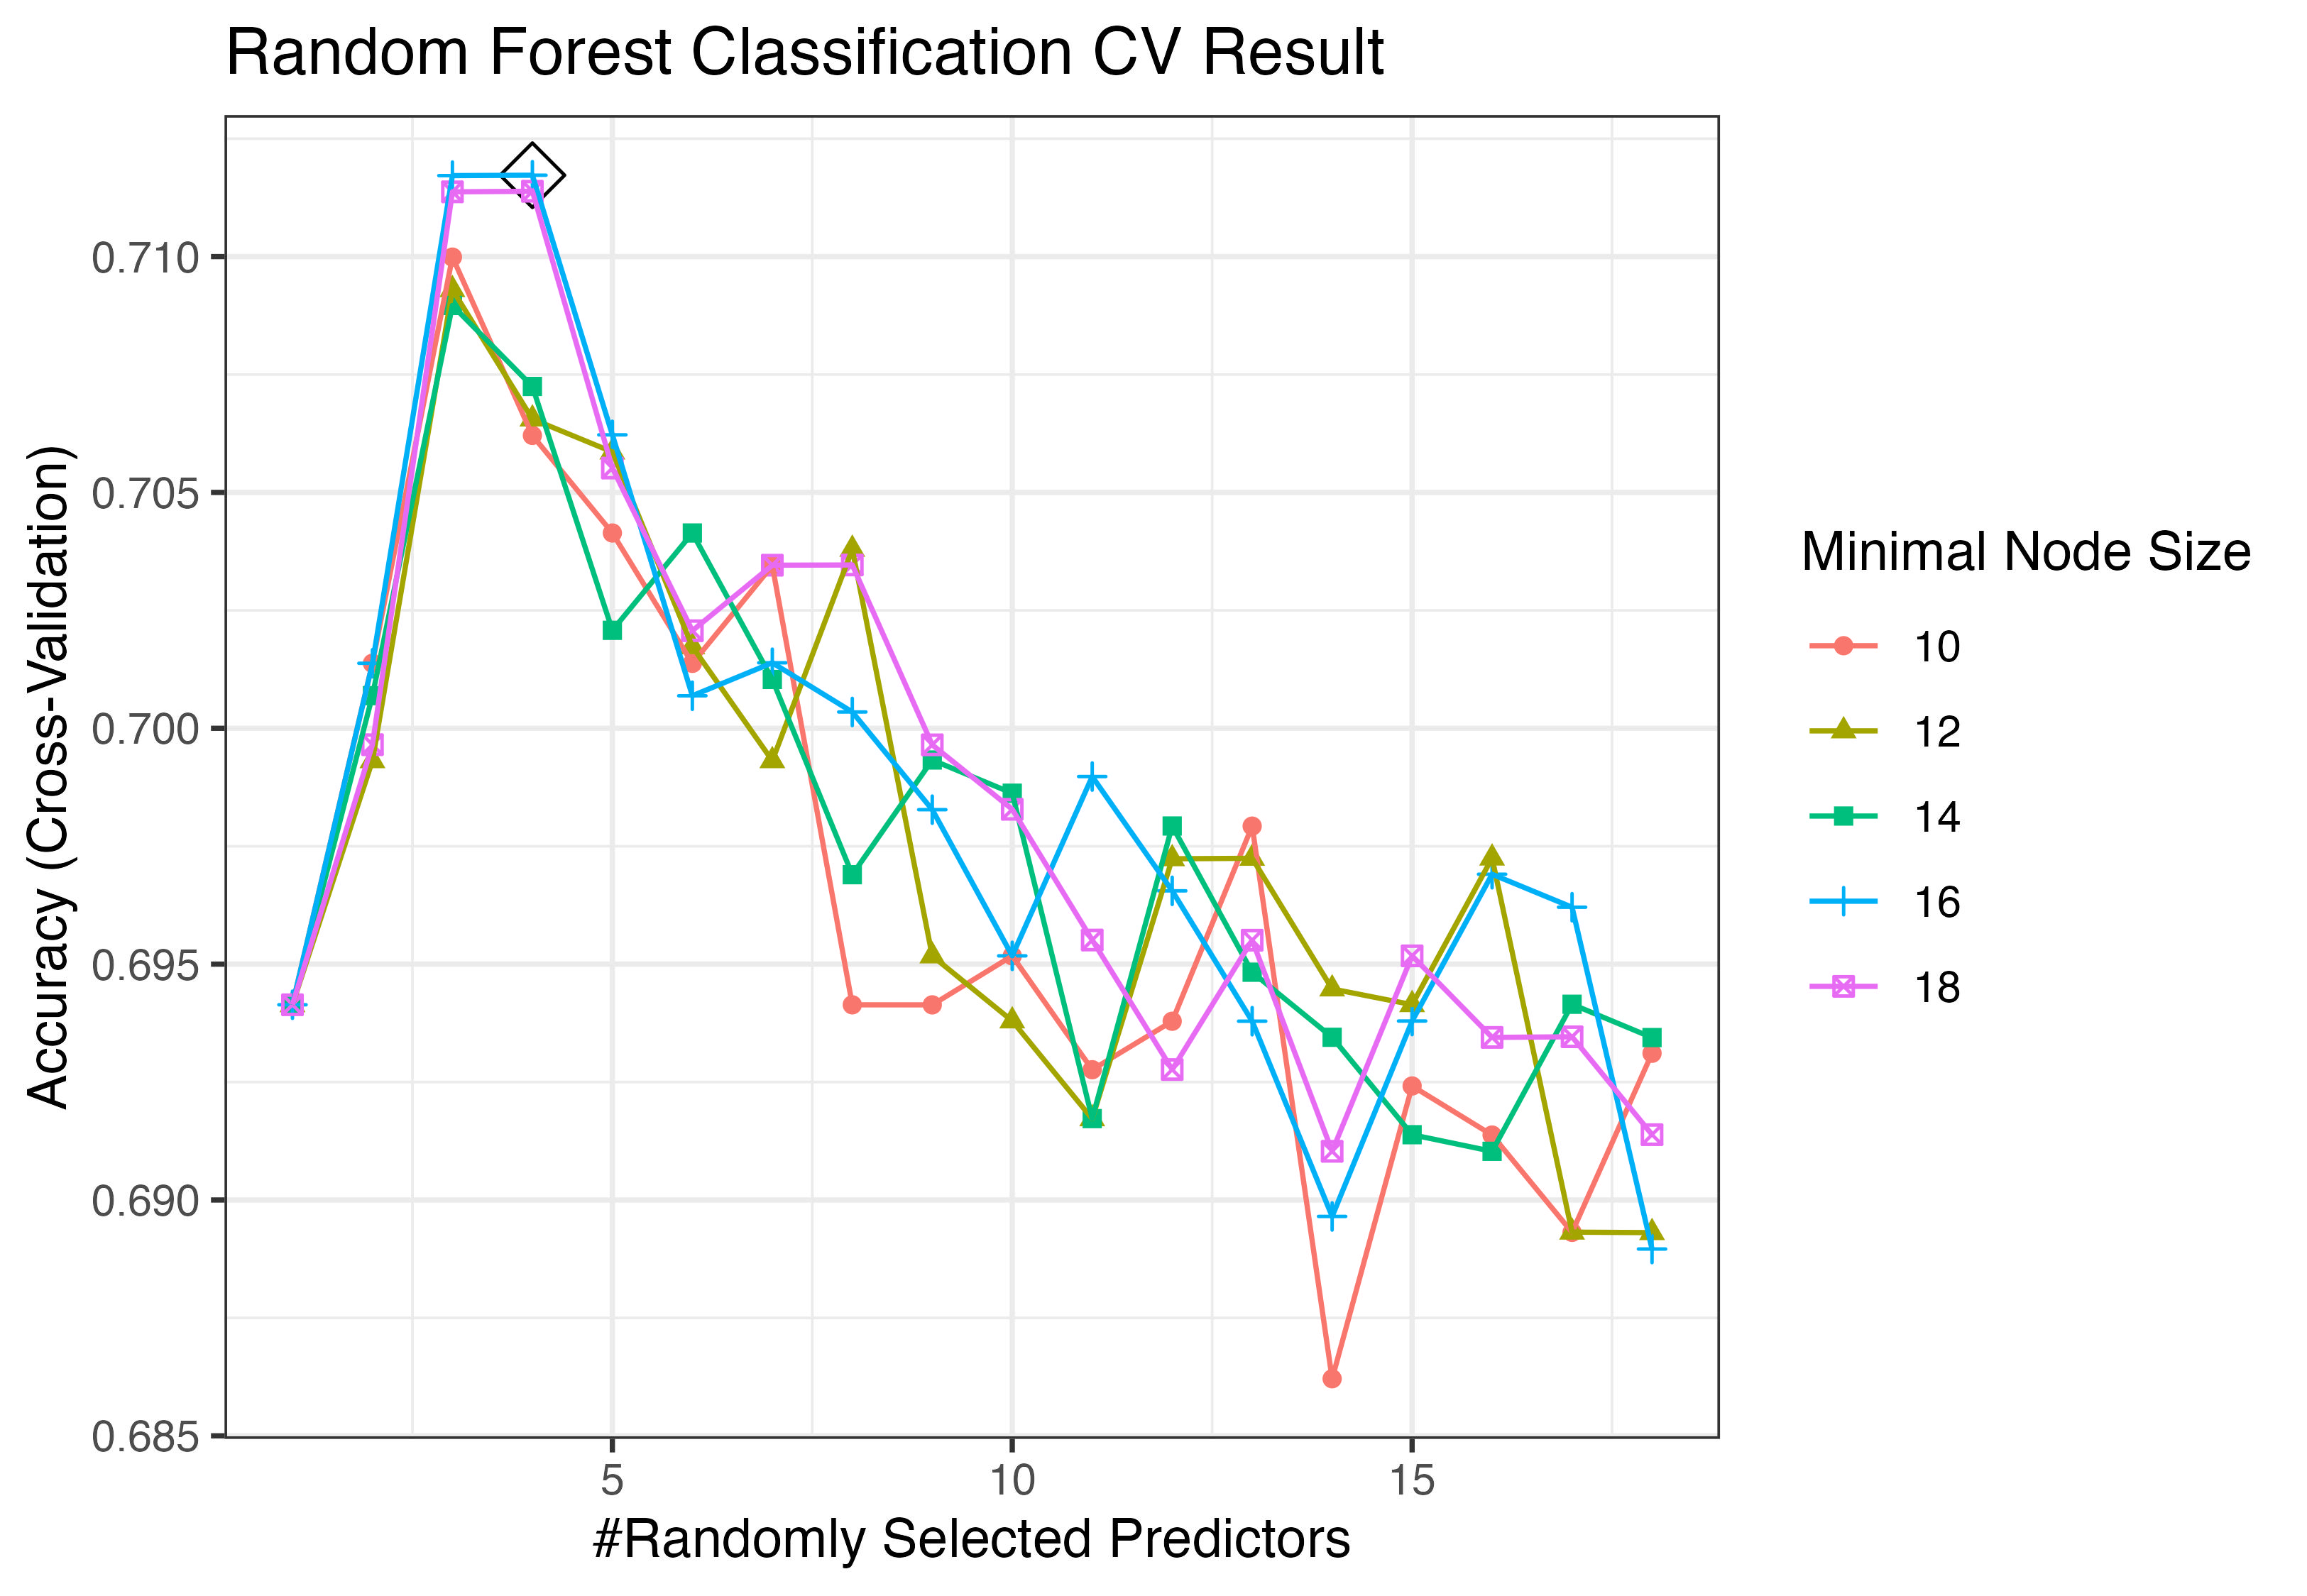
\includegraphics[width=0.32\textwidth]{secondary/rf_classification_cv.jpeg}\label{fig:rf_bin}}

    % 1
    \subfigure[Boosting]{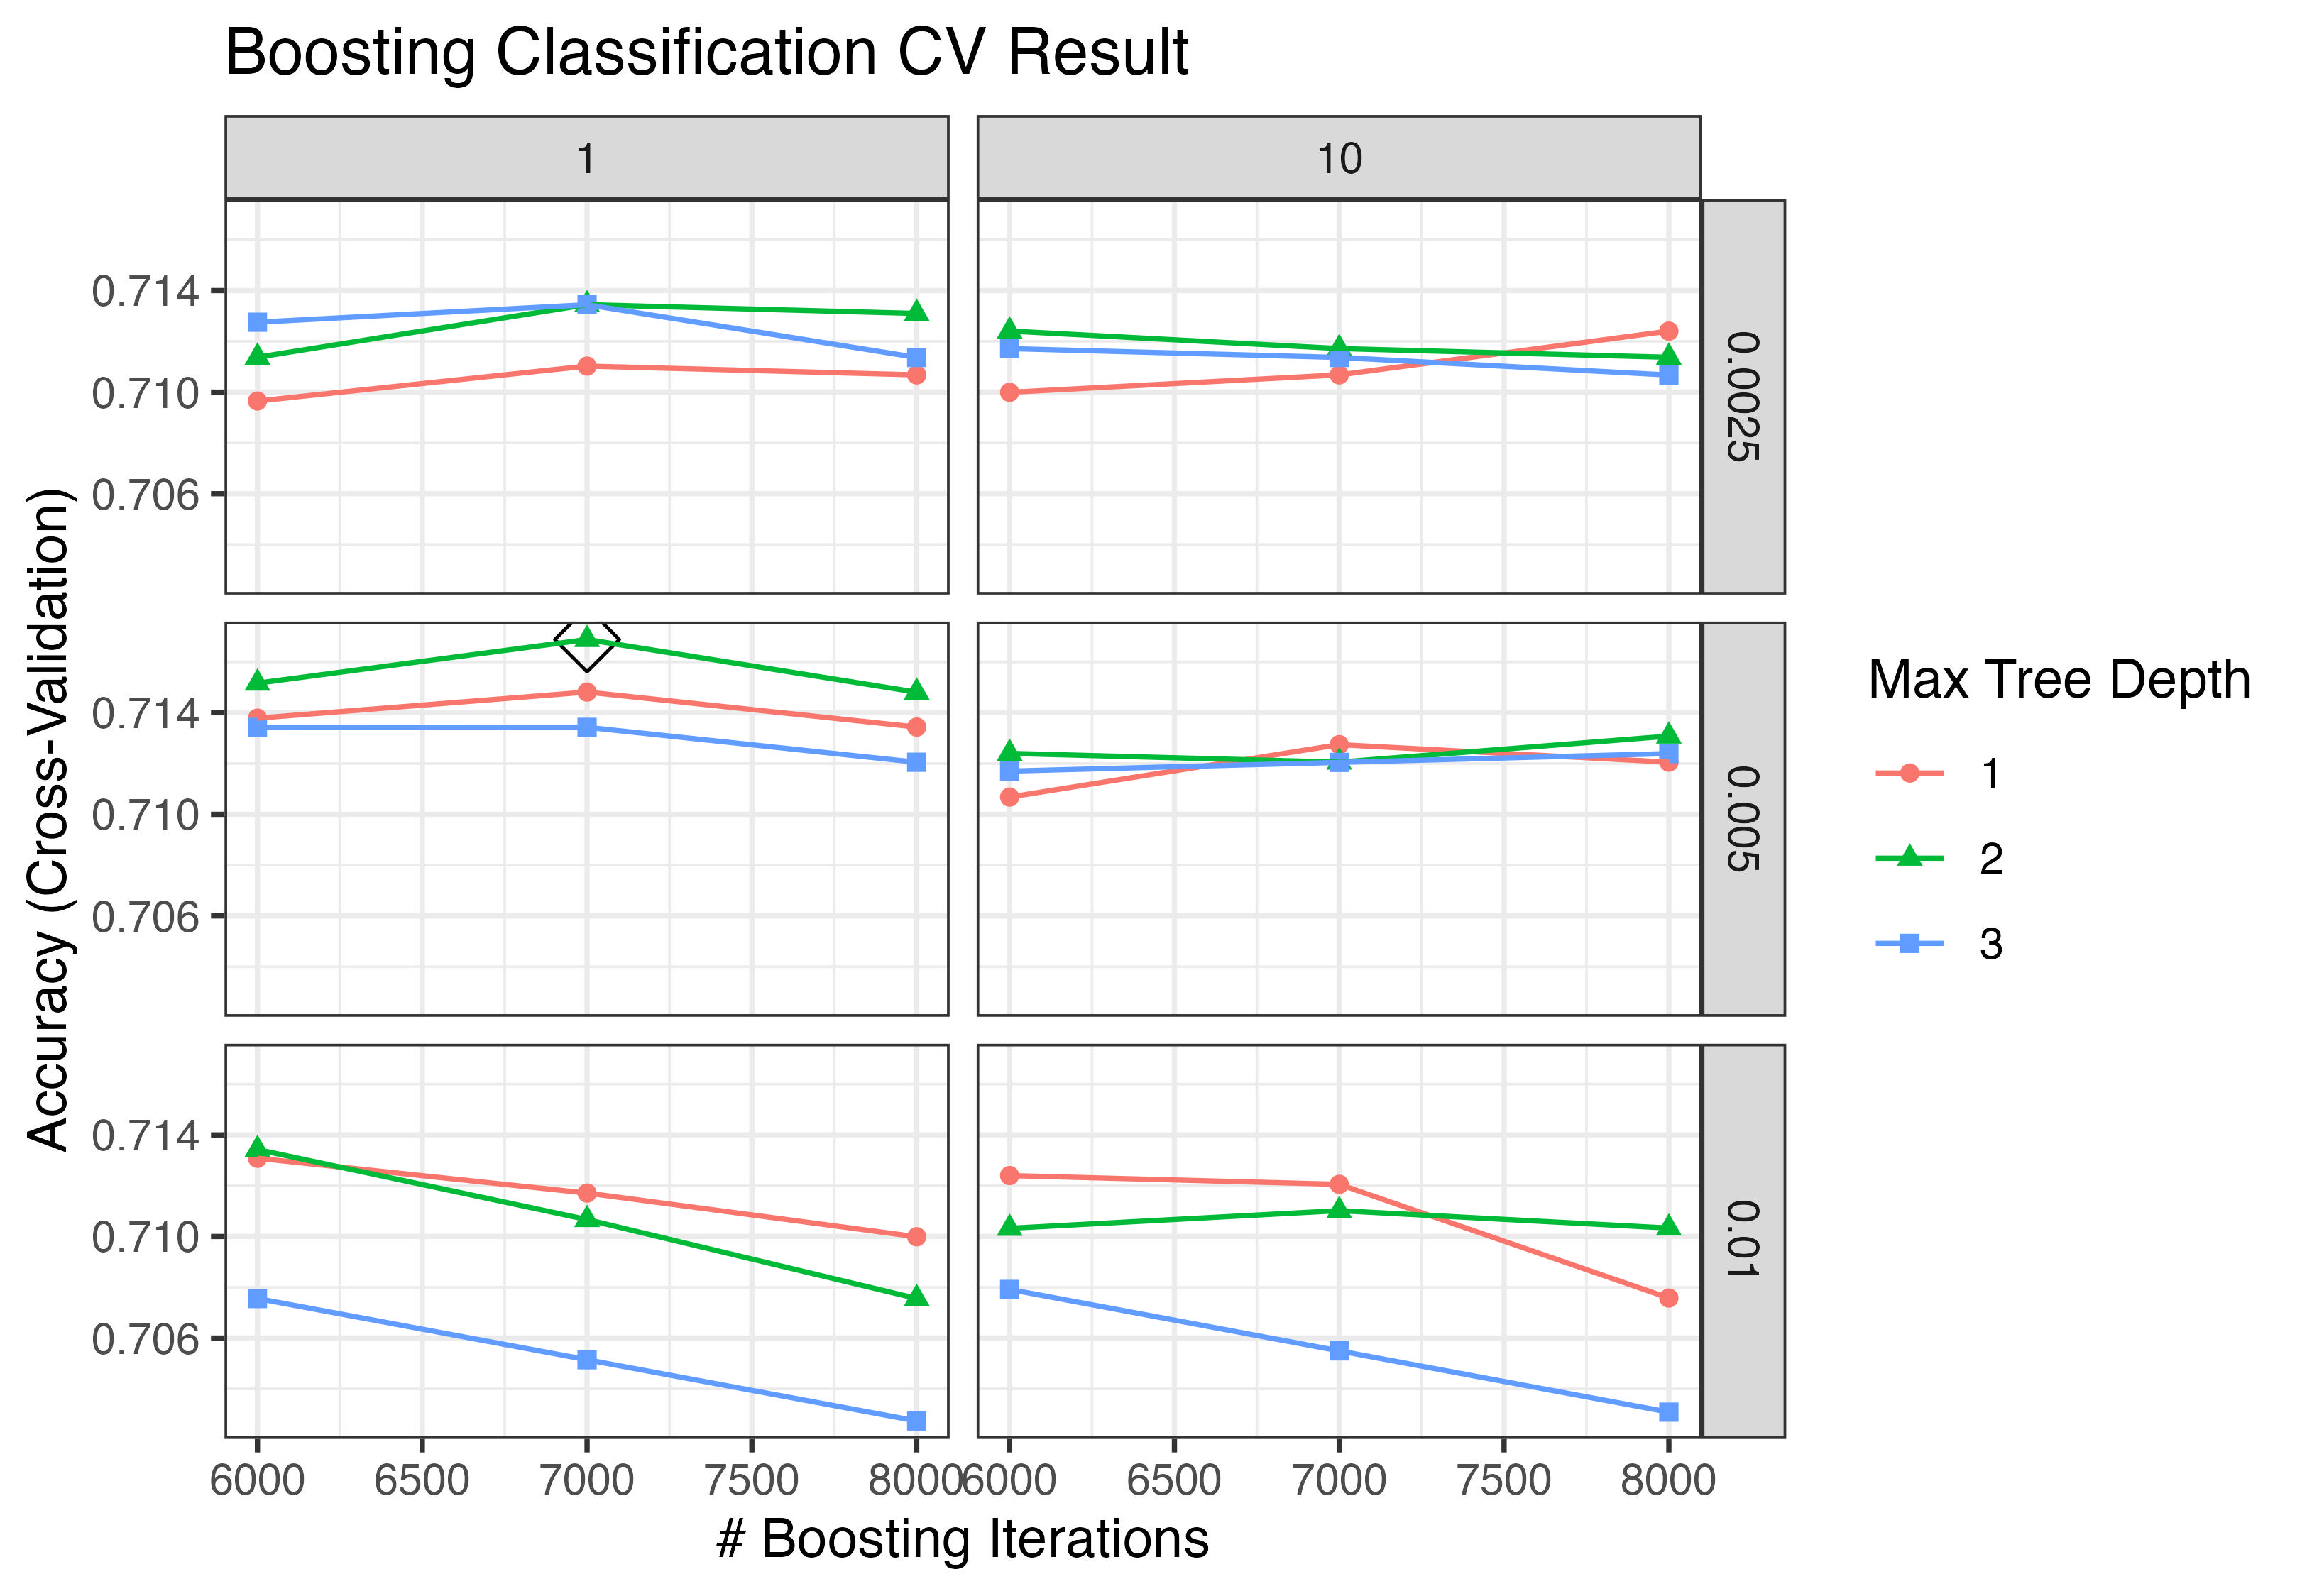
\includegraphics[width=0.32\textwidth]{secondary/boosting_classification_cv.jpeg}\label{fig:boosting_bin}}
    \hspace{0.1cm}
    % 2
    \subfigure[Classification tree]{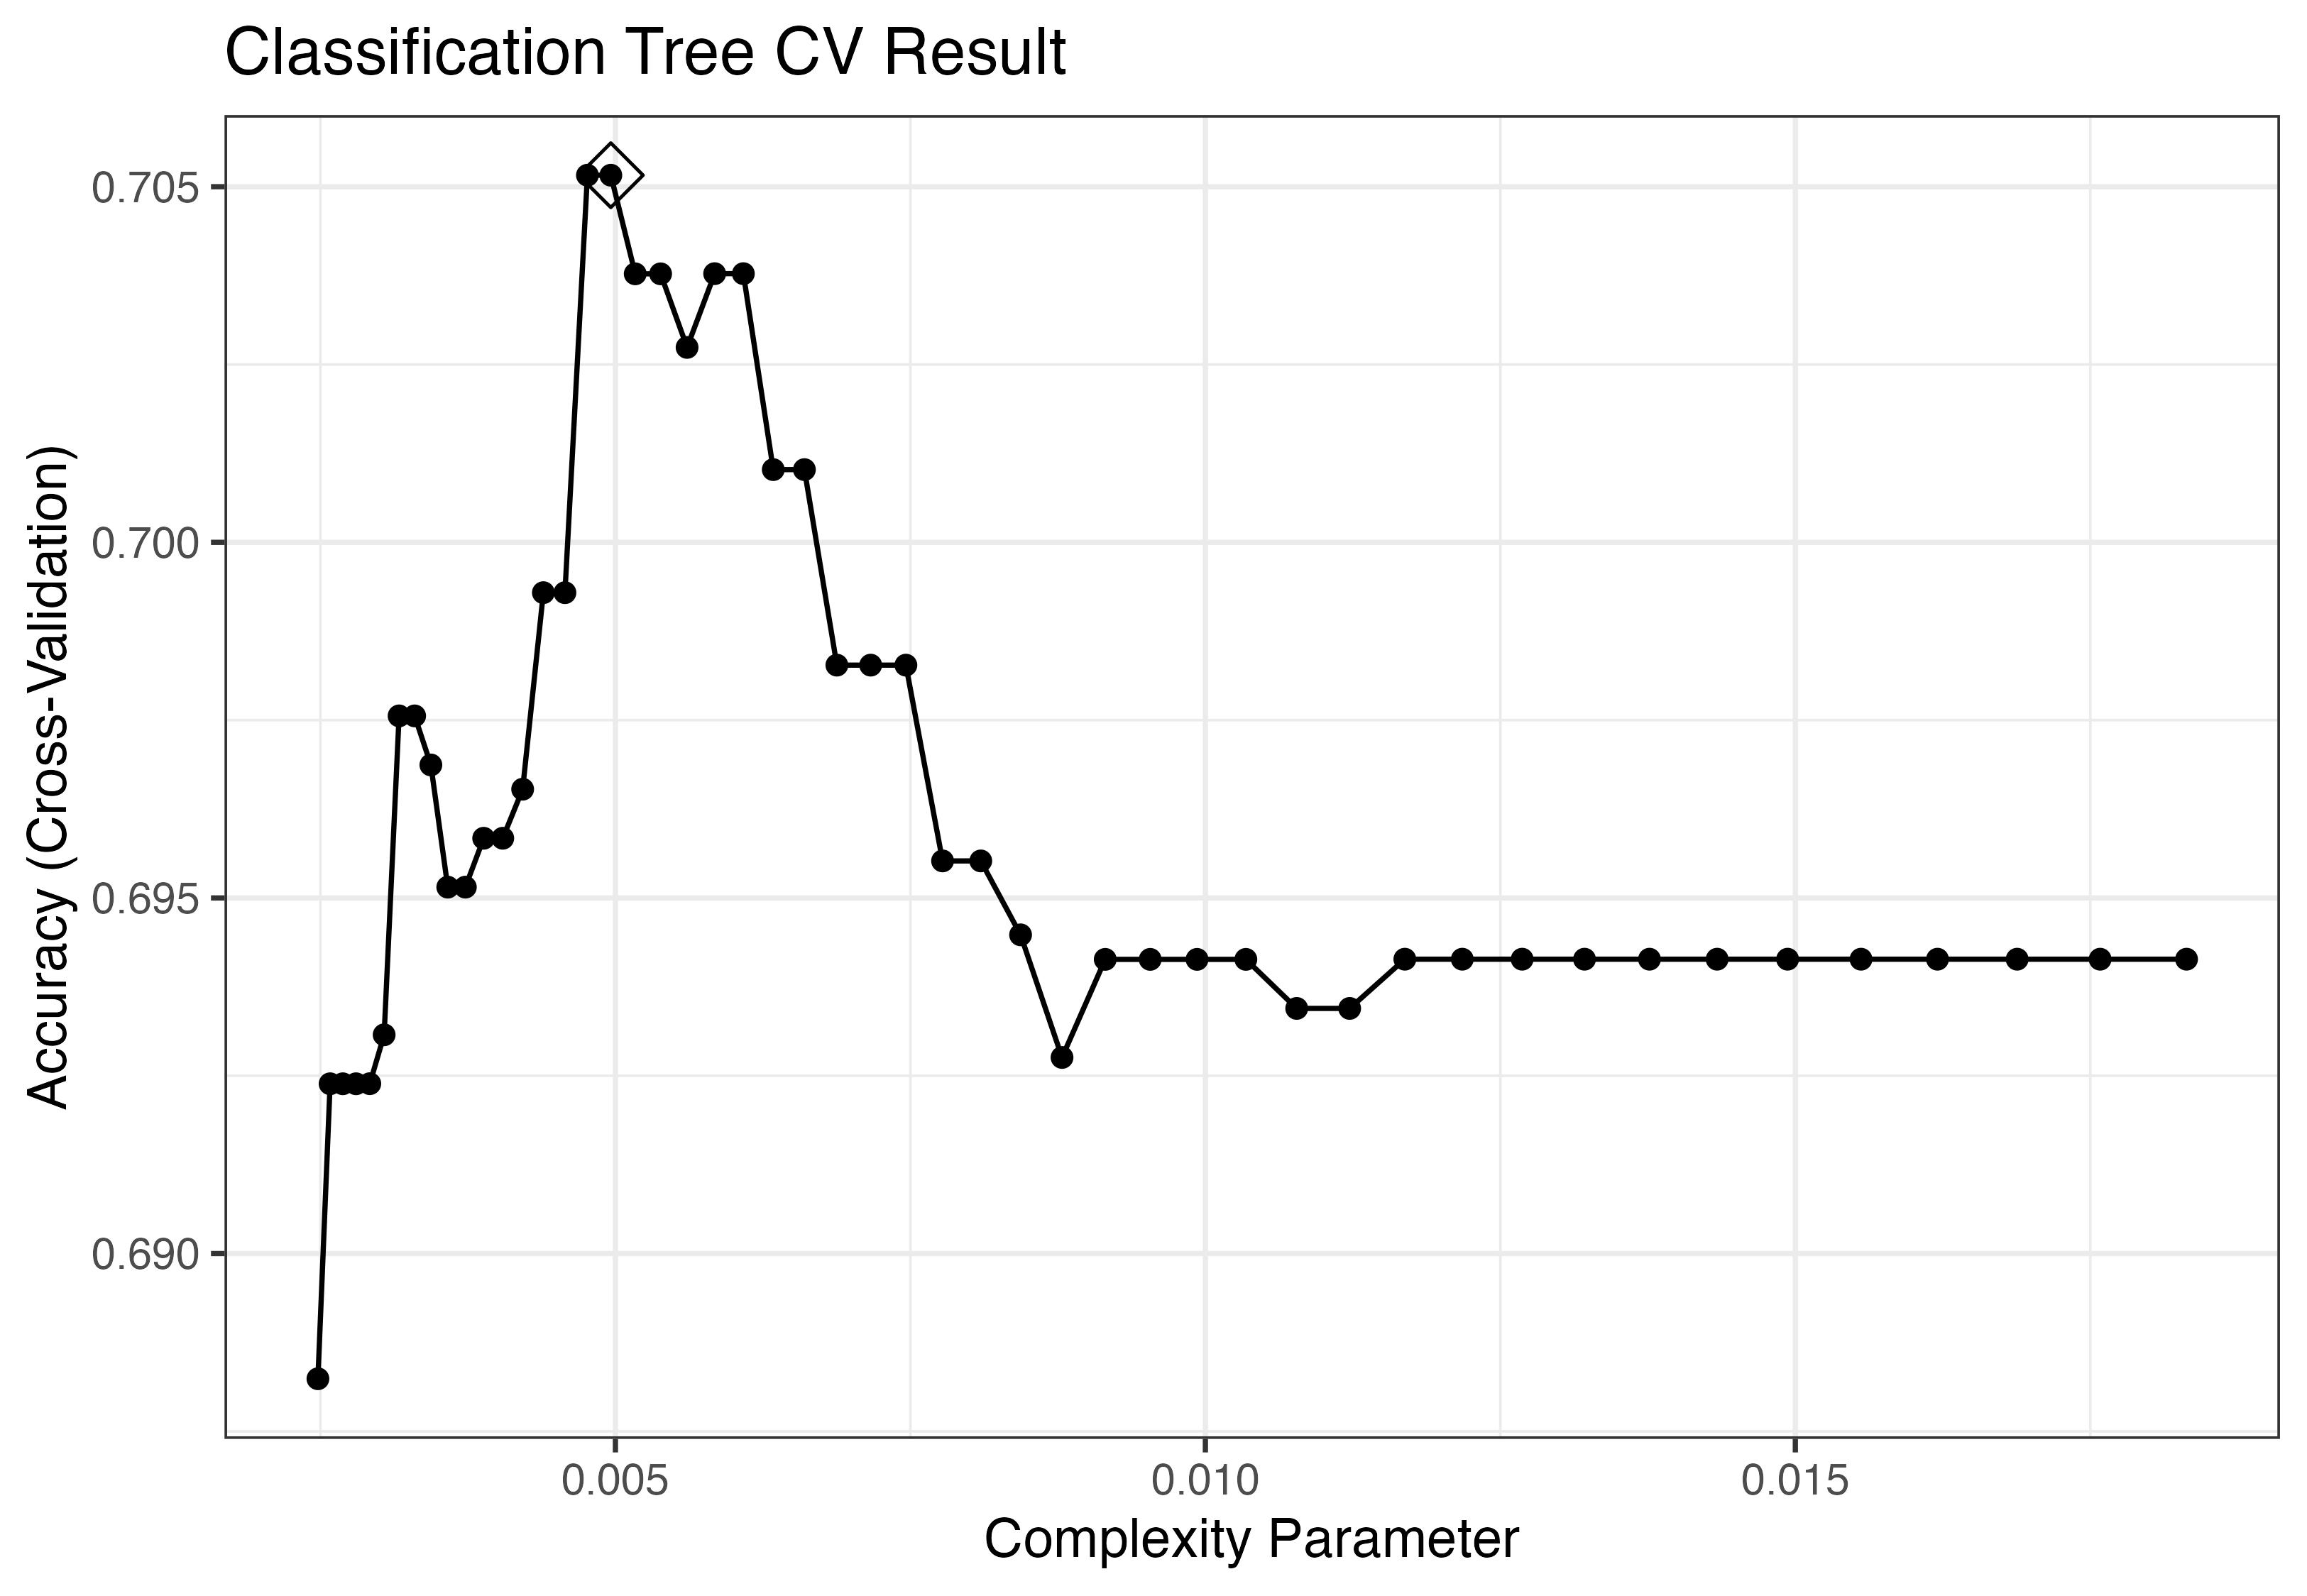
\includegraphics[width=0.32\textwidth]{secondary/rpart2_cv.jpeg}\label{fig:classtree}}
    \hspace{0.1cm}
    % 3
    \subfigure[SVMR]{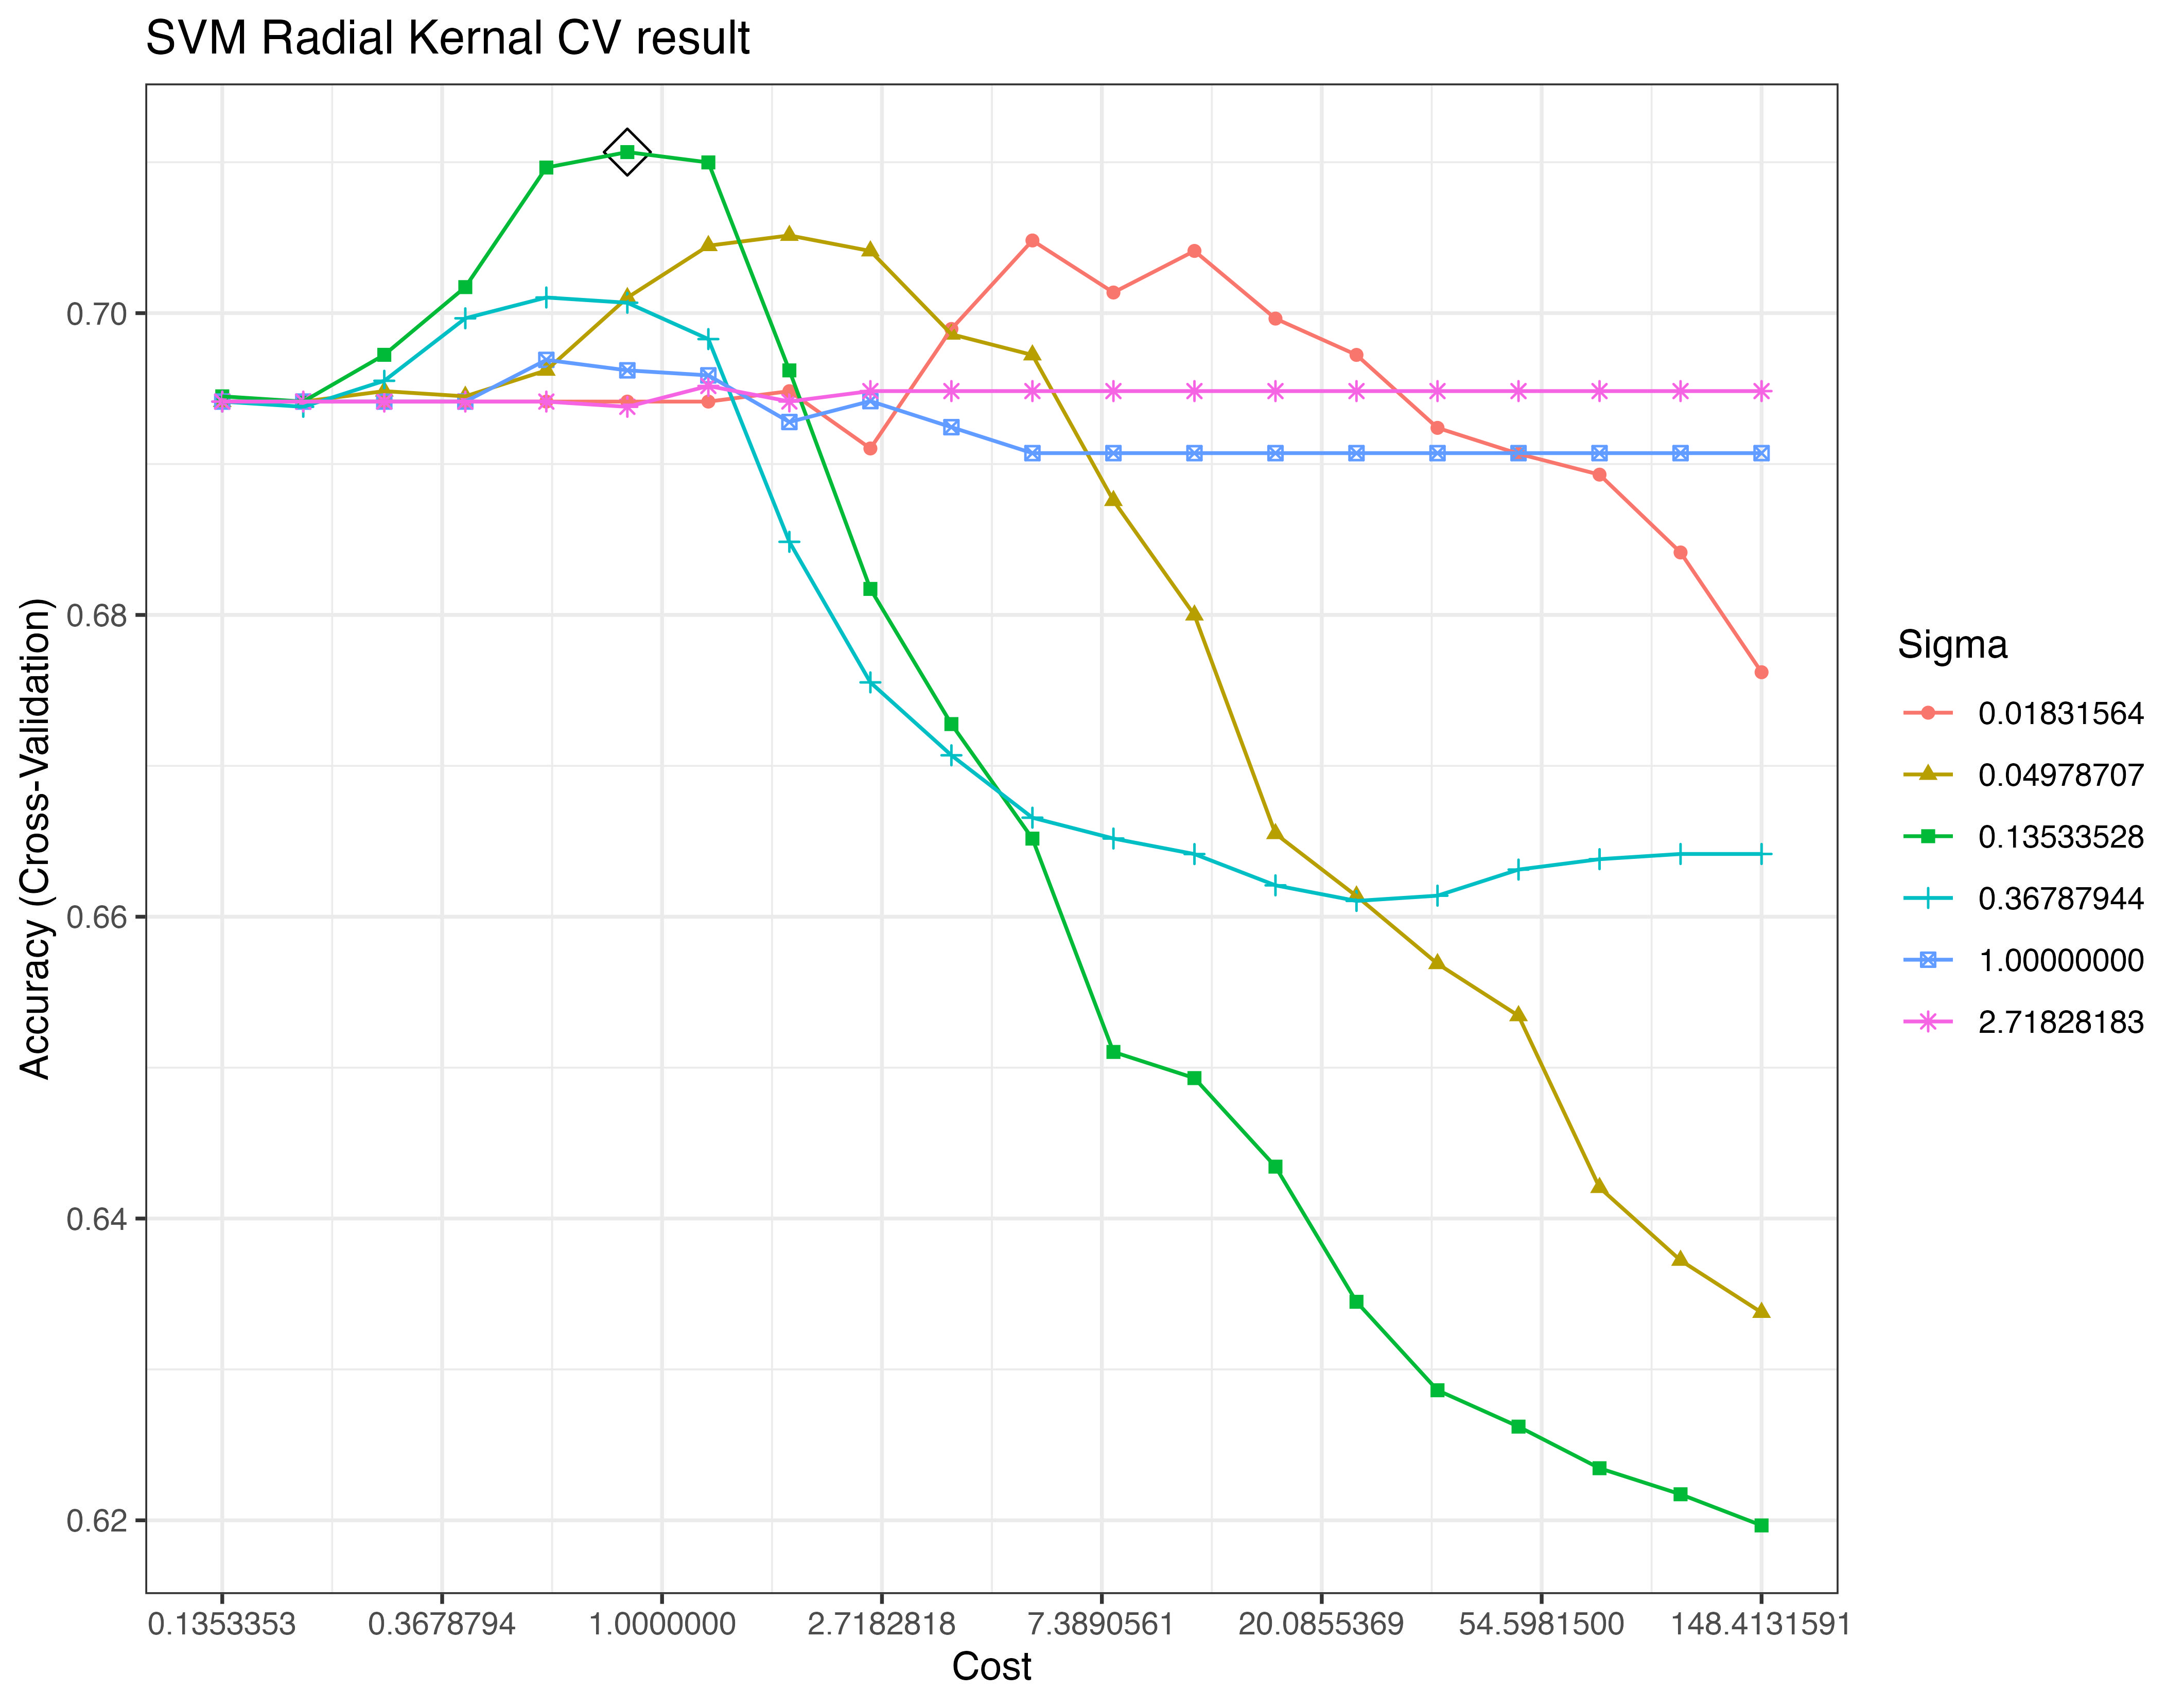
\includegraphics[width=0.32\textwidth]{secondary/svmr_cv.jpeg}\label{fig:svmr}}
    
    \caption{Secondary analysis CV results}
    \label{fig:secondary}
\end{figure}


\begin{figure}
    \centering
     % 1
    \subfigure[Primary analysis]{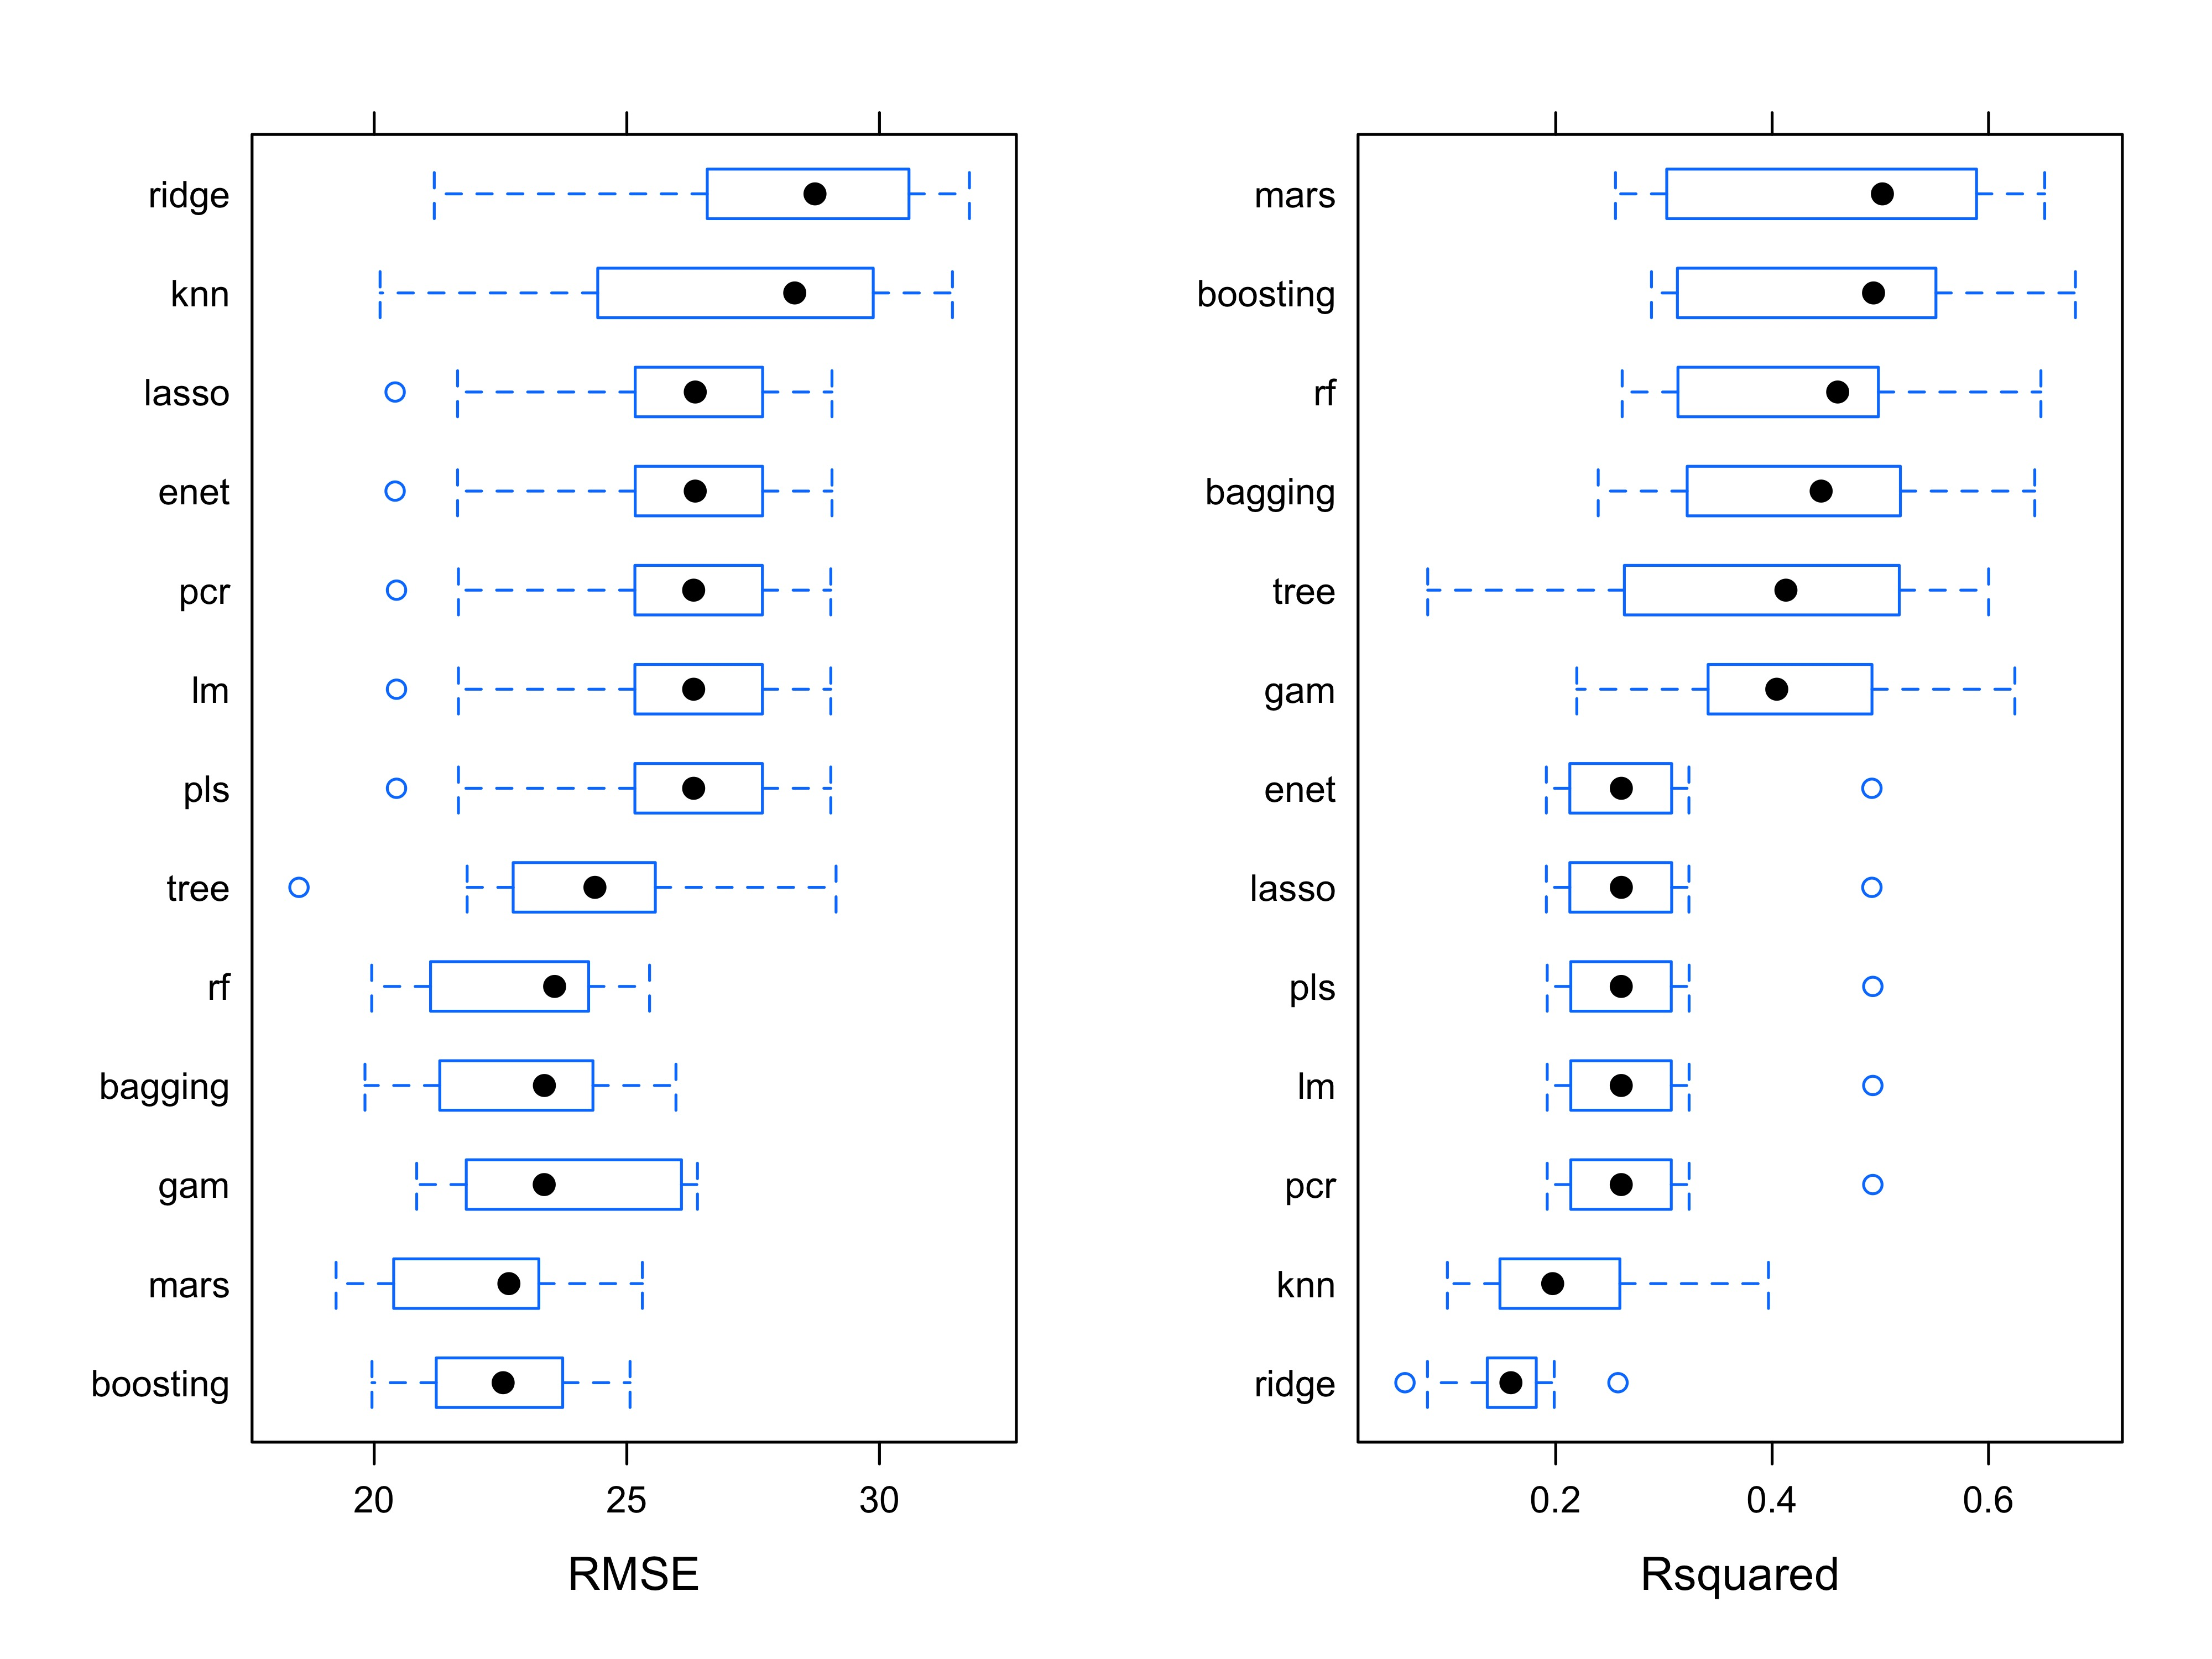
\includegraphics[width=0.8\textwidth]{primary/resample1.jpeg}\label{fig:resample1}}

    % 2
    \subfigure[Secondary analysis]{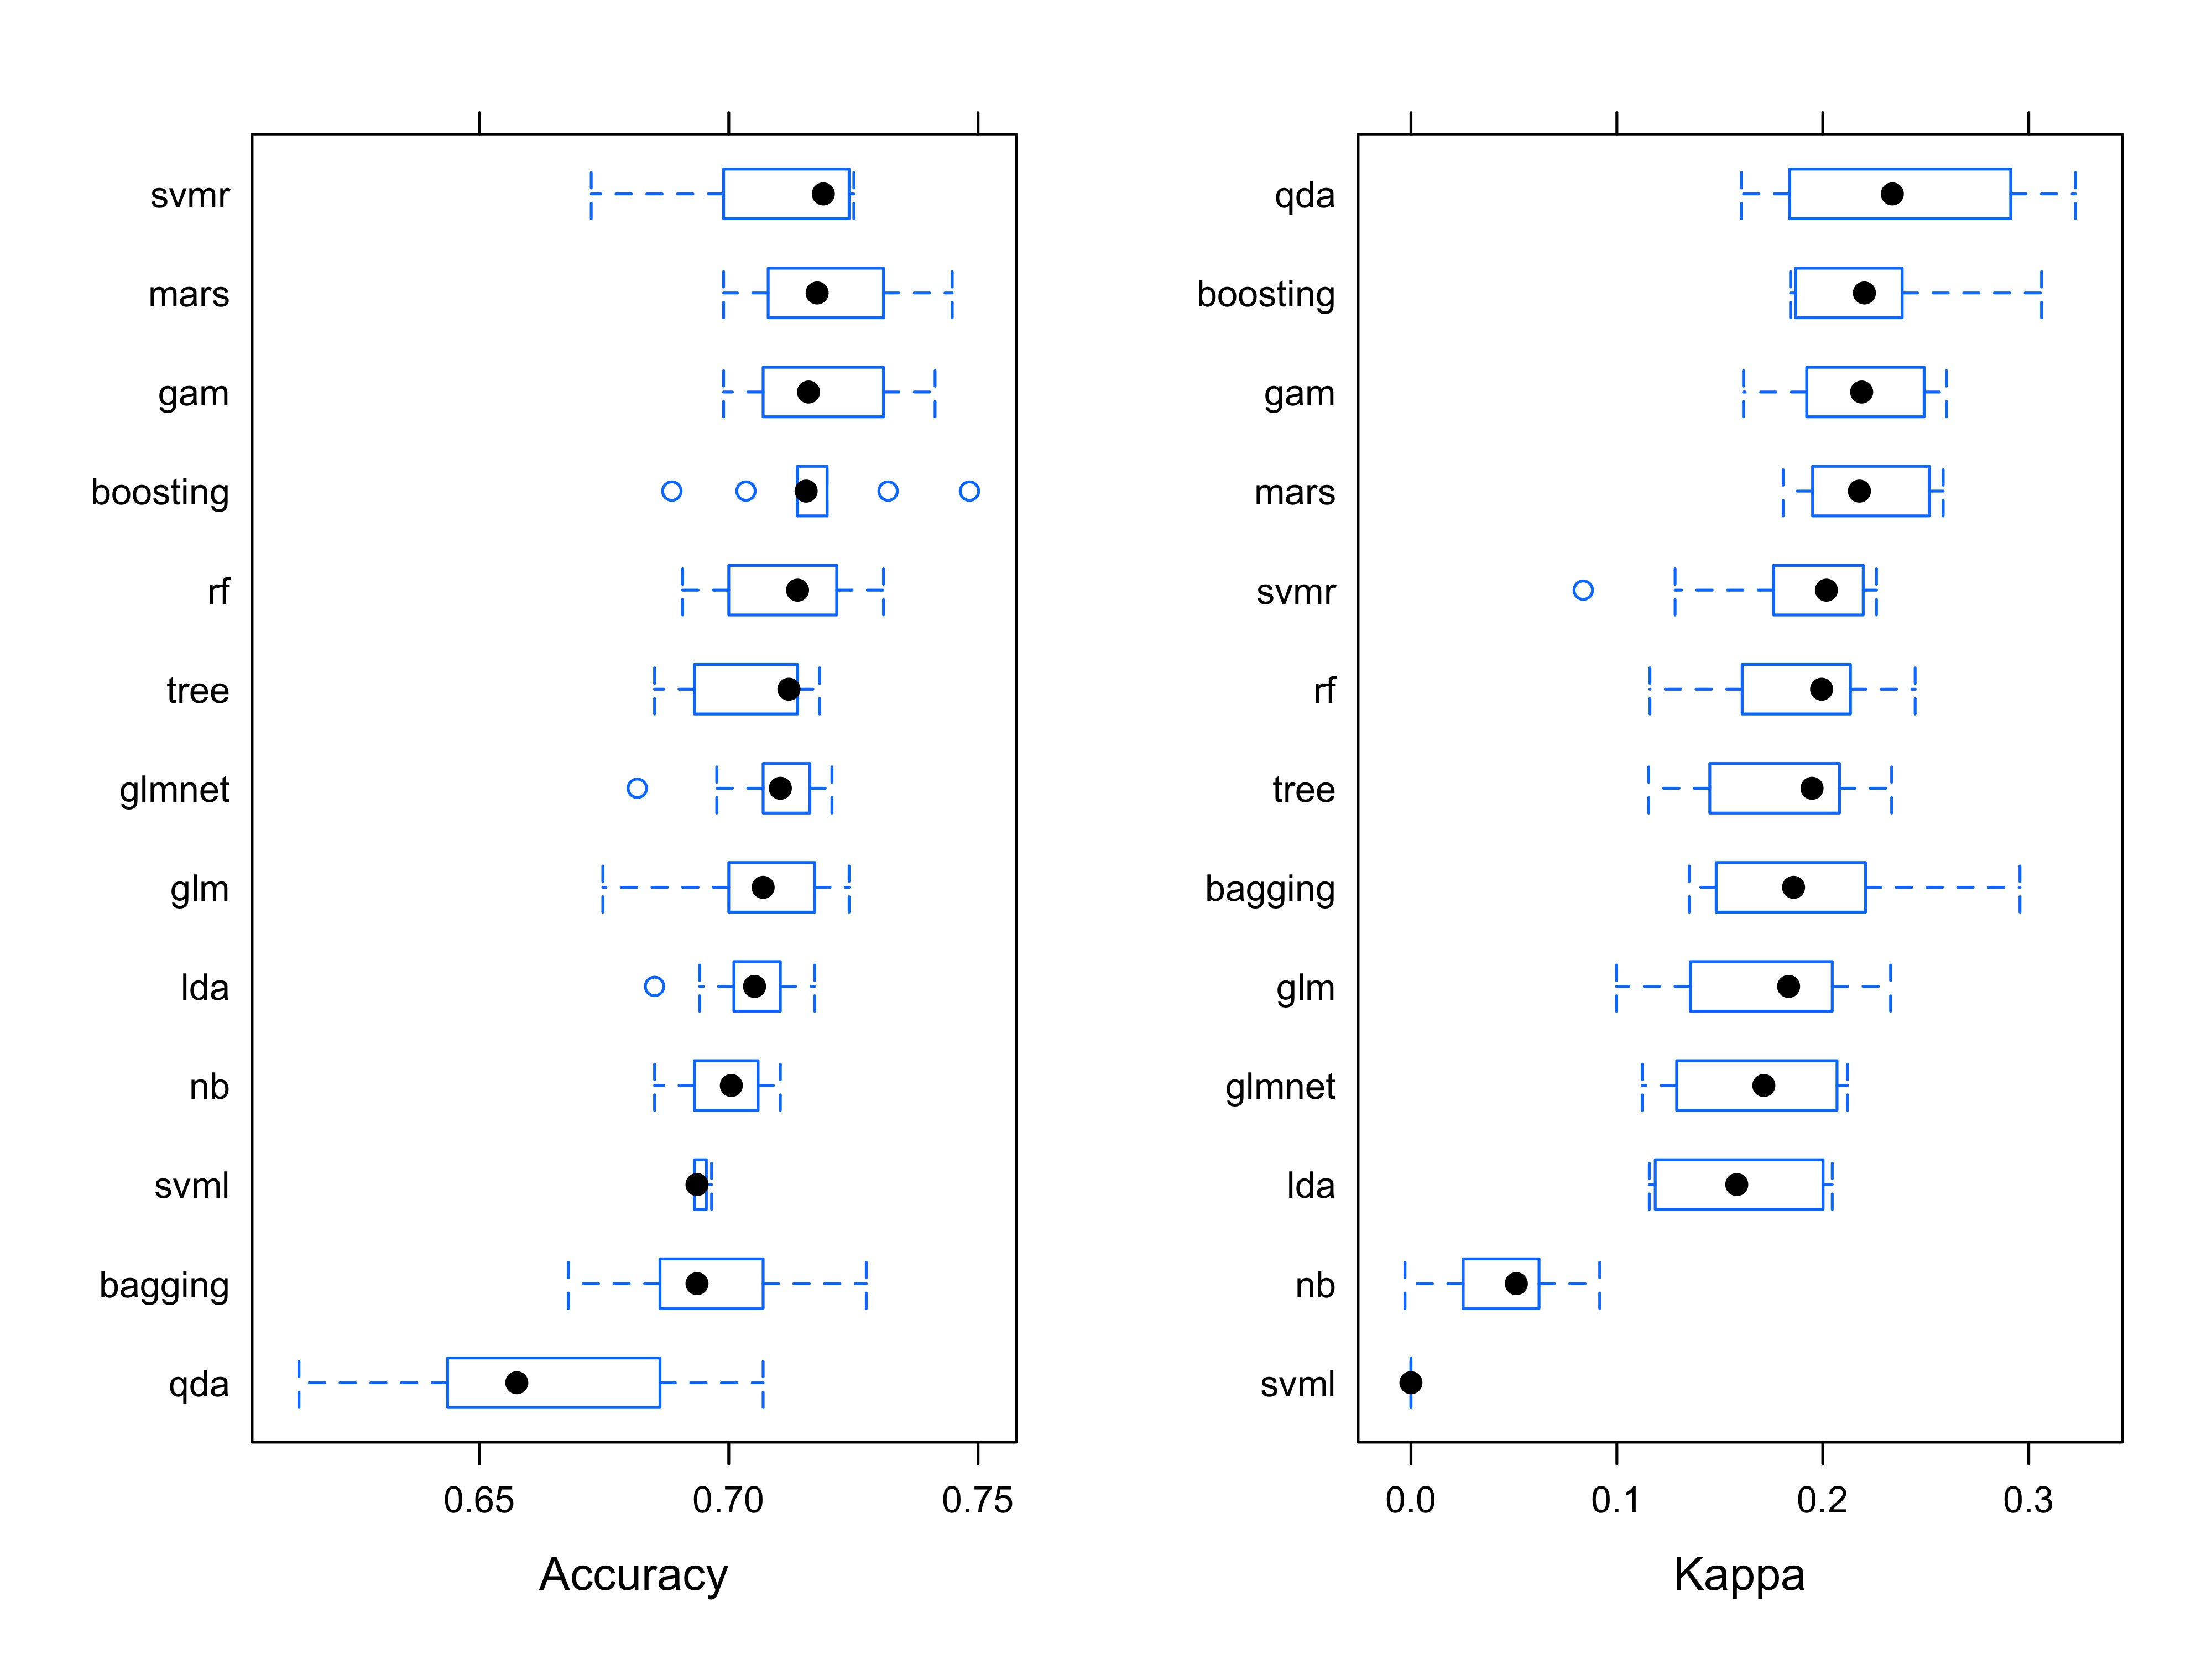
\includegraphics[width=0.8\textwidth]{secondary/resample2.jpeg}\label{fig:resample2}}

    \caption{Resample results}
    \label{fig:resample}
\end{figure}

\begin{figure}
    \centering
     % 1
    \subfigure[Variable importance scores]{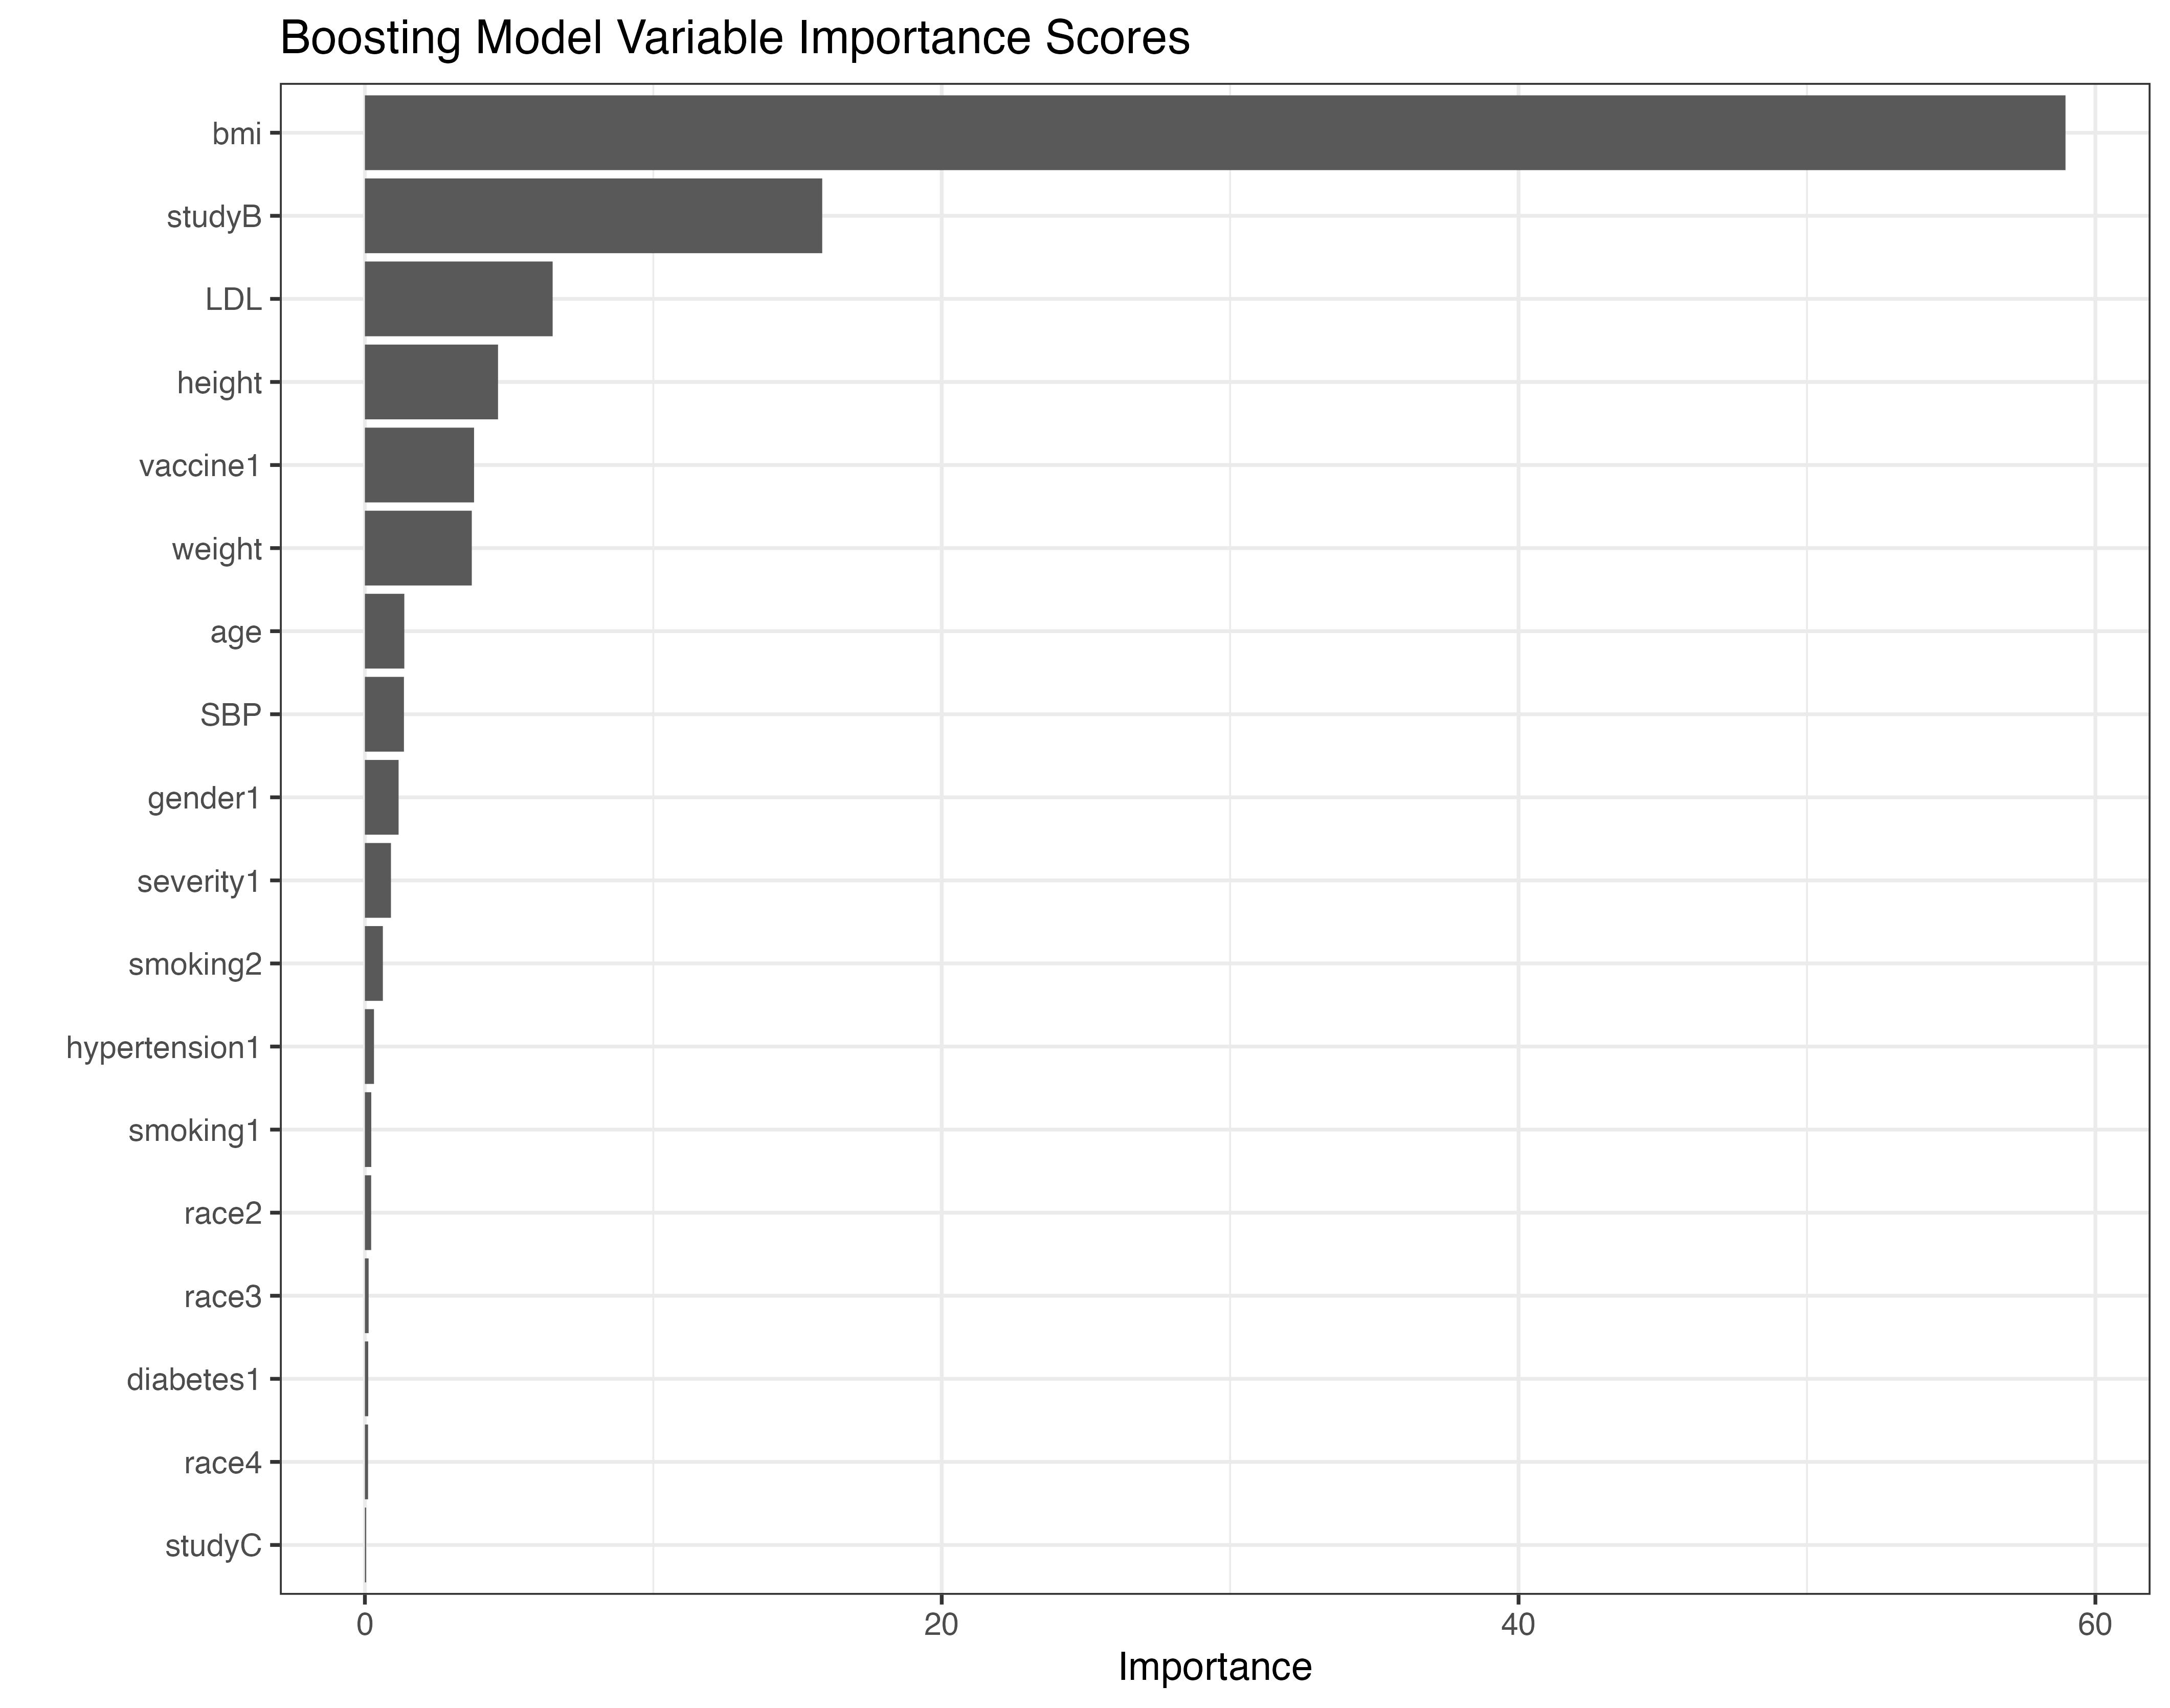
\includegraphics[width=0.8\textwidth]{result/boosting_vip.jpeg}\label{fig:boostingvip}}
    % 2
    \subfigure[Partial dependence plots]{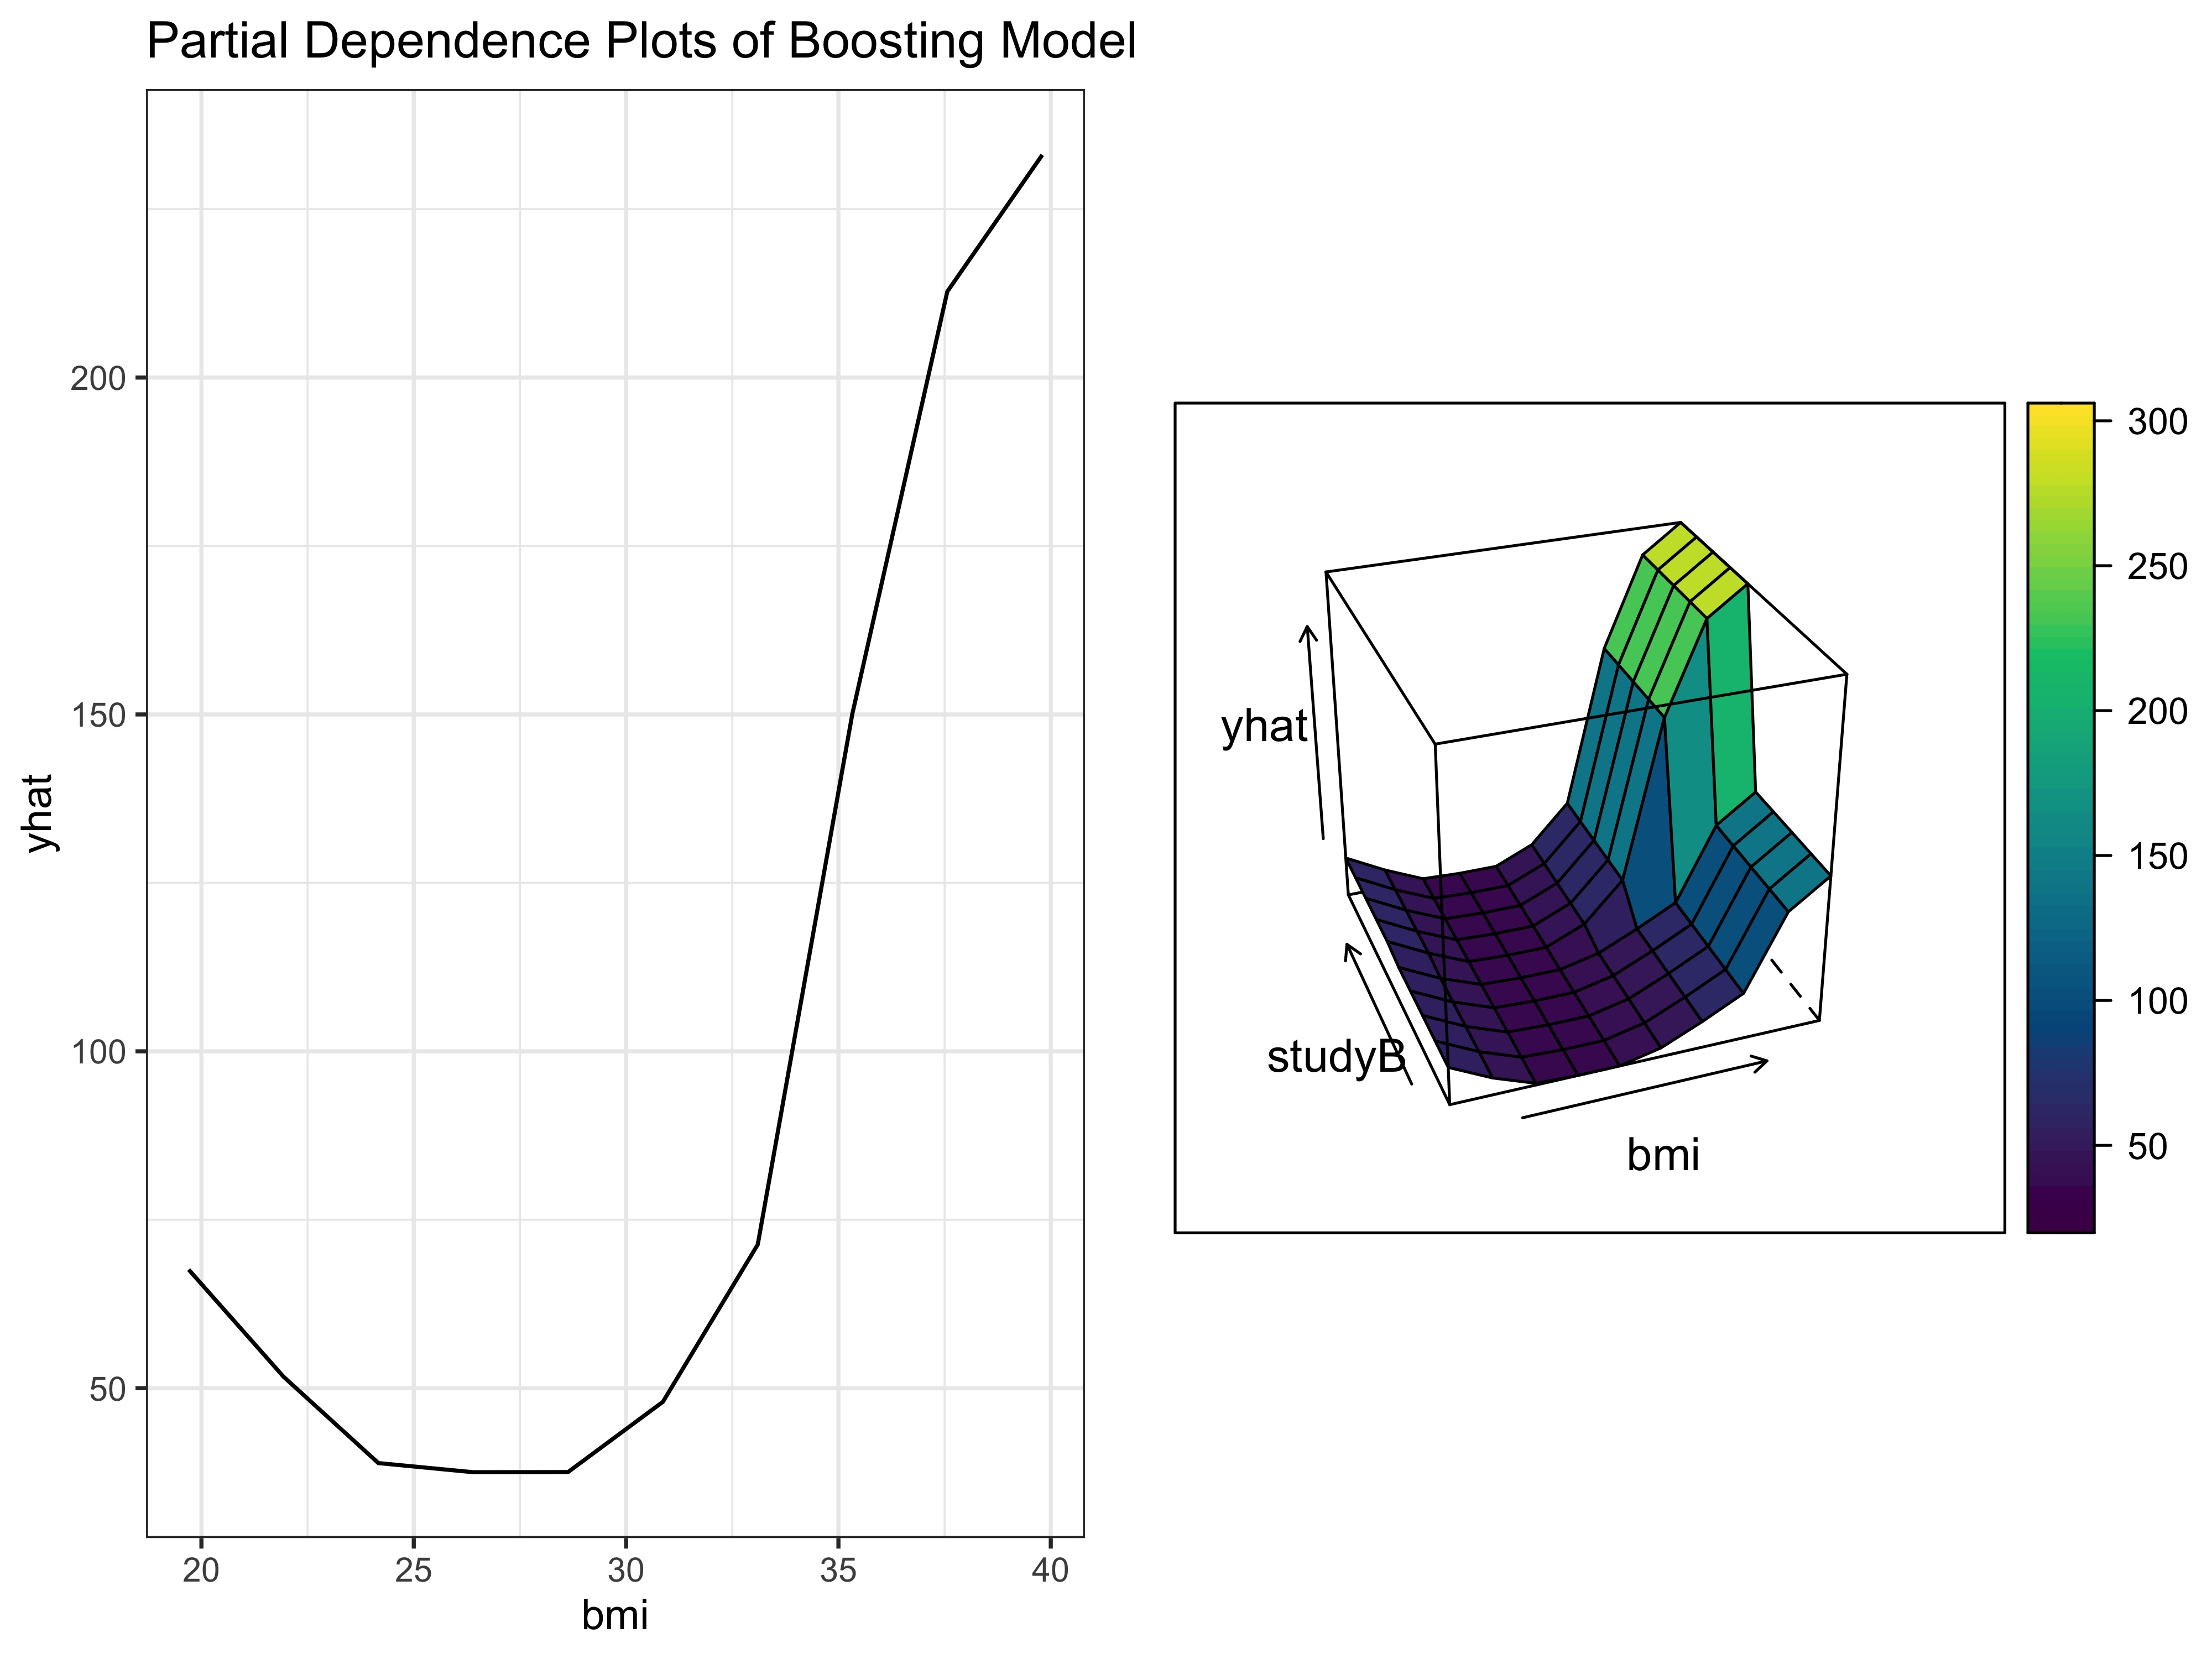
\includegraphics[width=0.8\textwidth]{result/partial_dependence.jpeg}\label{fig:boostingpdp}}
    \caption{Boosting model interpretation}
    \label{fig:bst}
\end{figure}

\begin{figure}
    \centering
     % 1
     \subfigure[Variable importance scores]{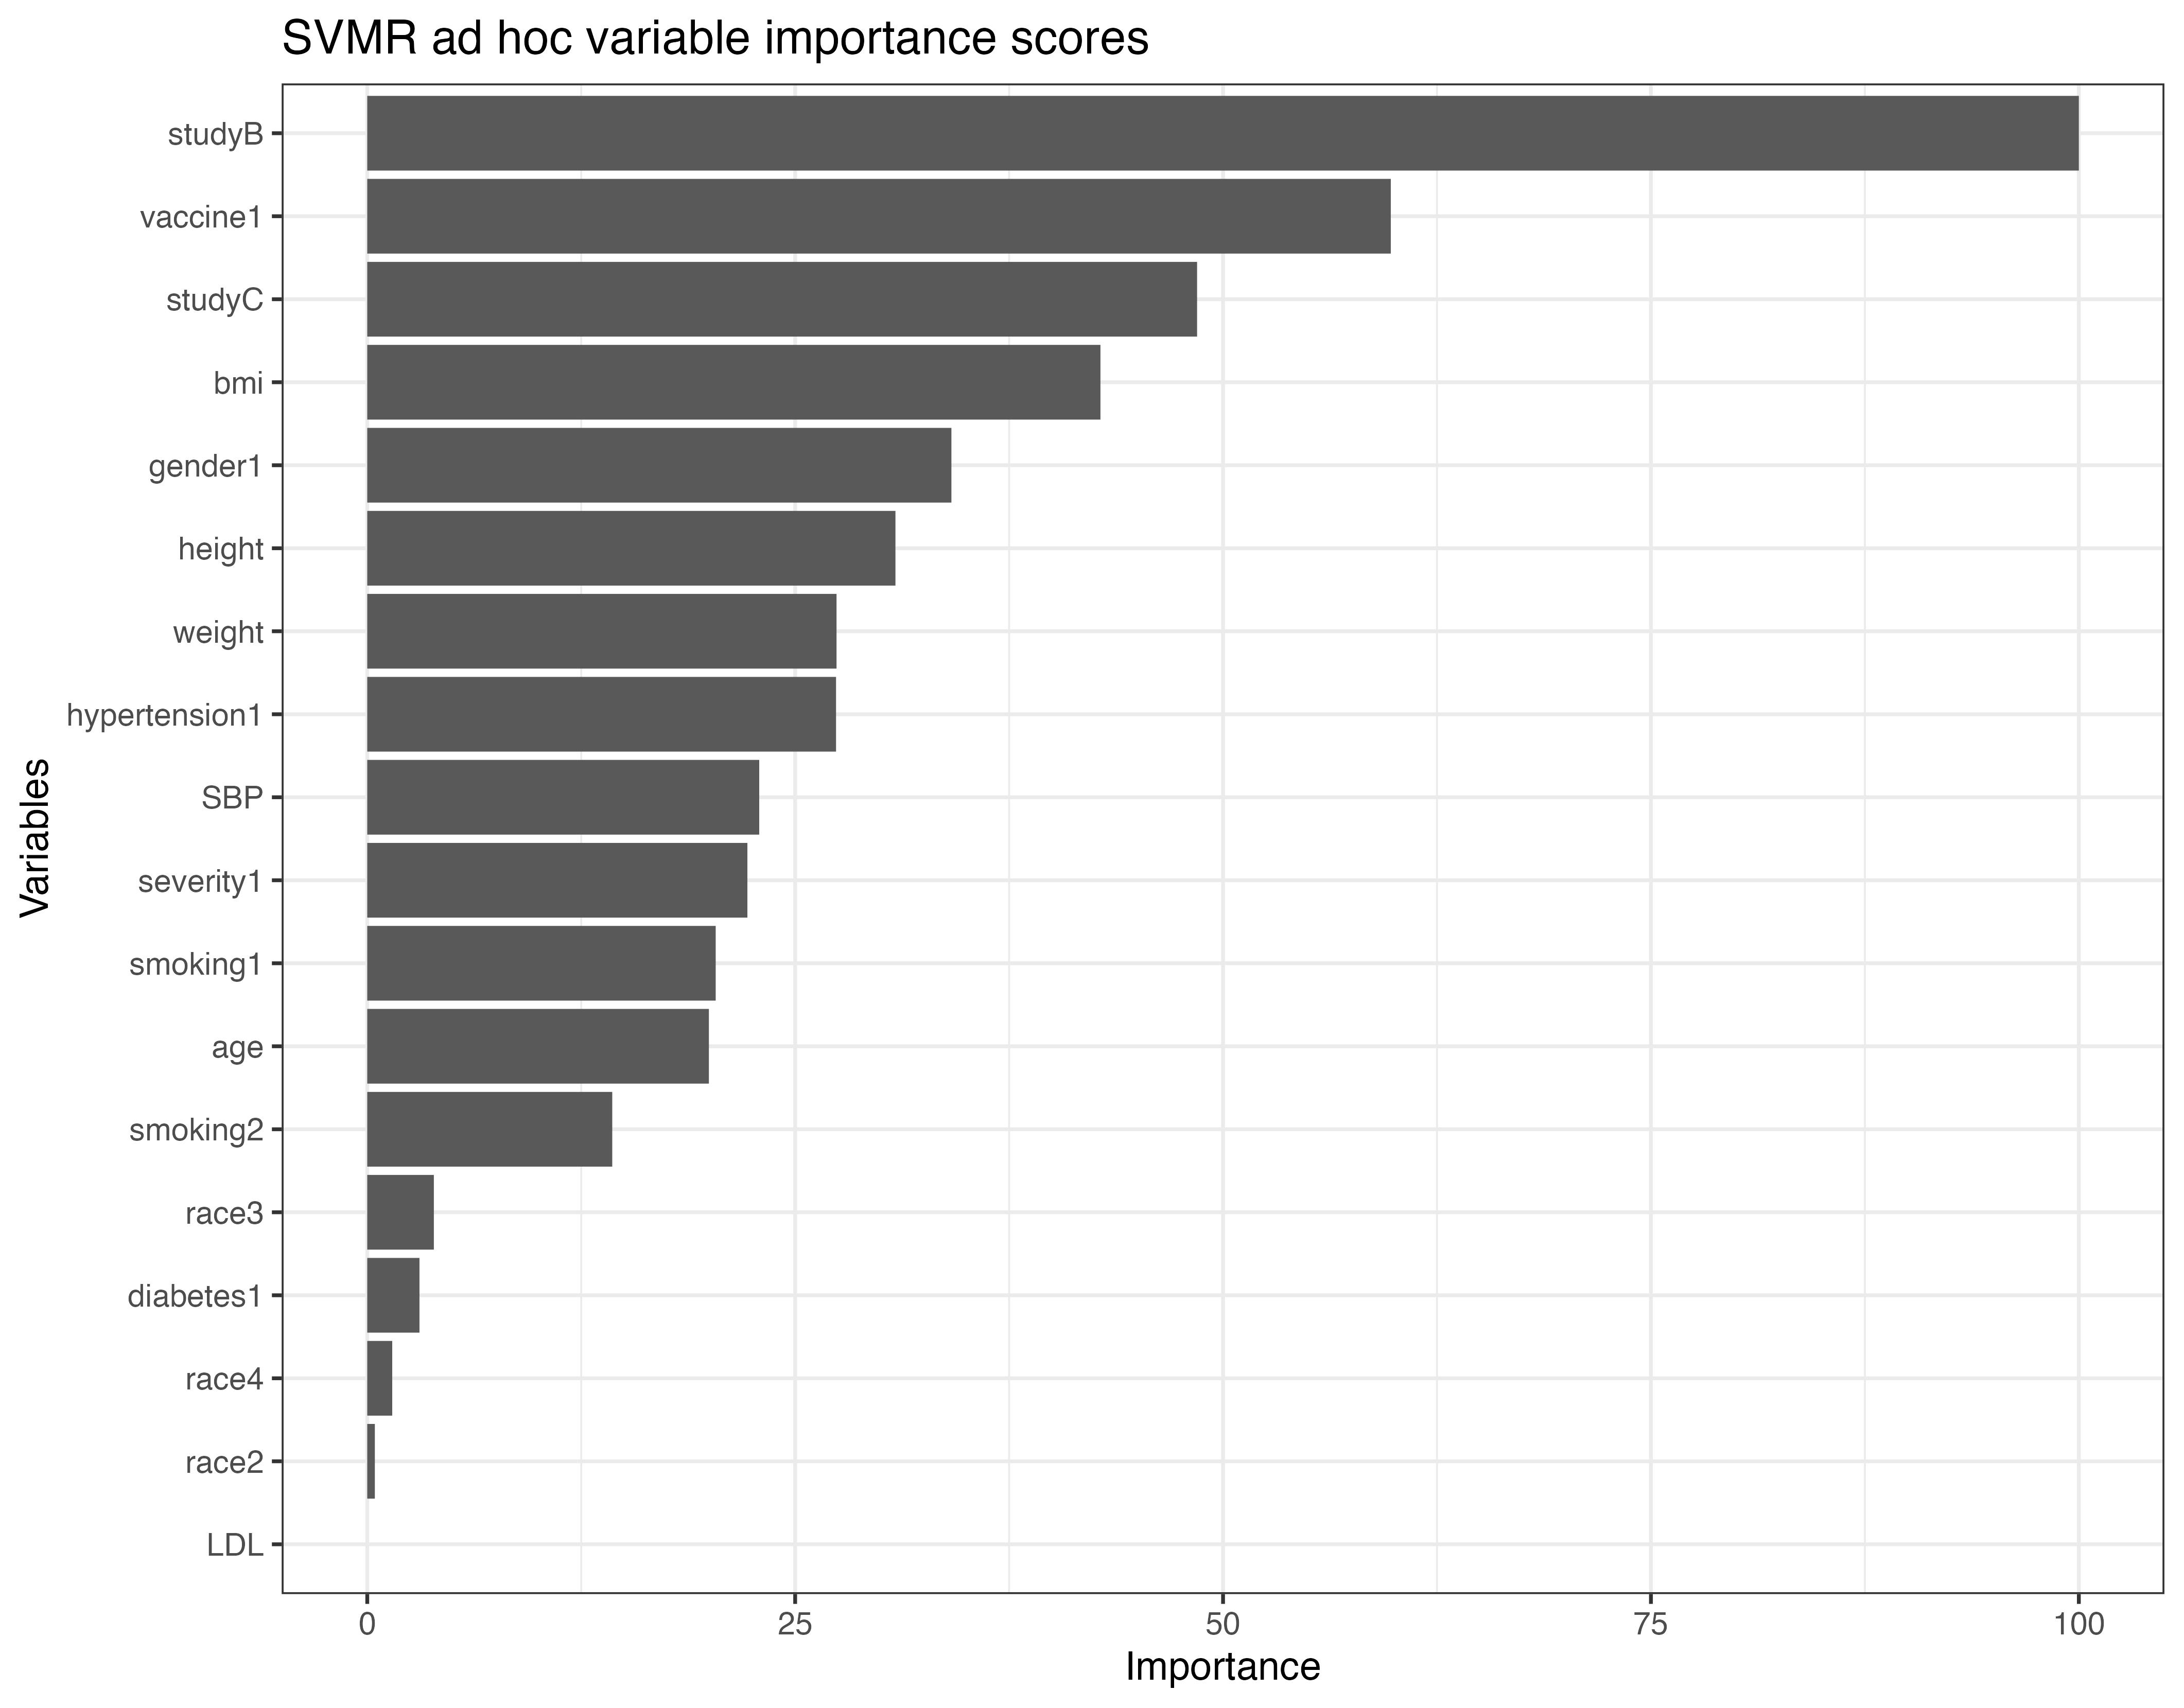
\includegraphics[width=0.8\textwidth]{result/svmr_vip.jpeg}\label{fig:svmrvip}}
    % 2
    \subfigure[Partial dependence plots]{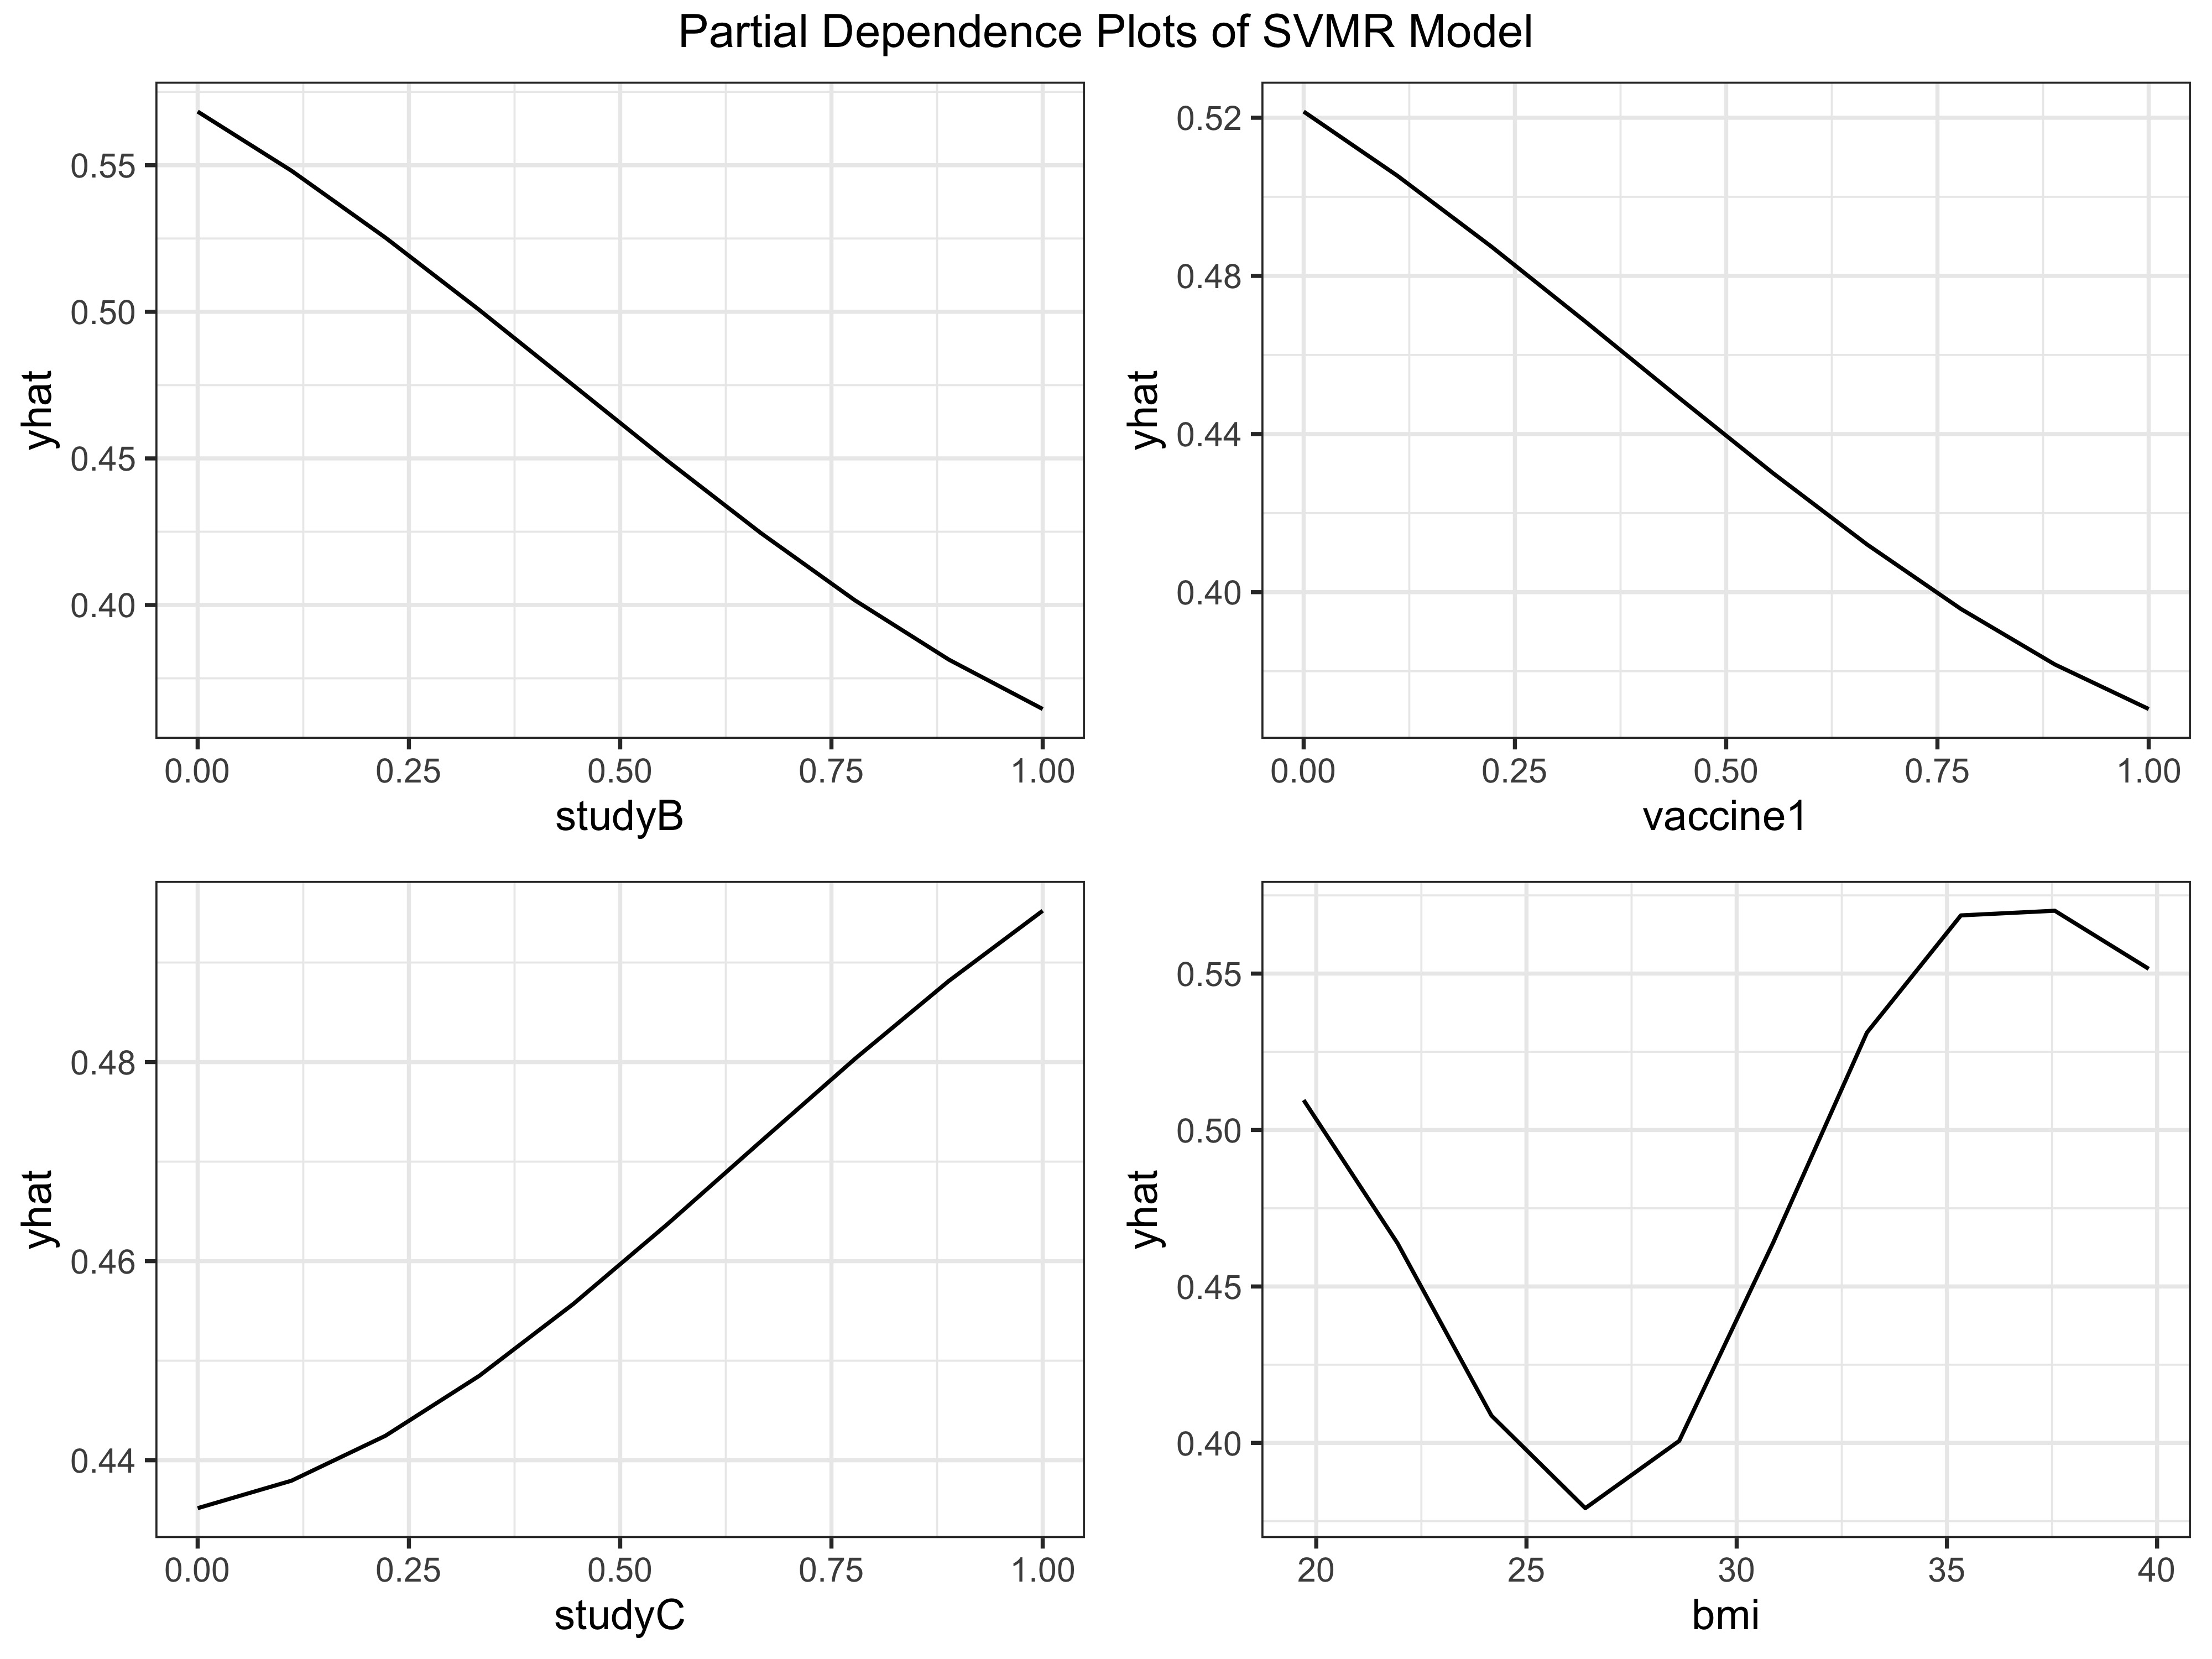
\includegraphics[width=0.8\textwidth]{result/svmr_pdp.jpeg}\label{fig:svmrpdp}}

    \caption{SVMR model interpretation}
    \label{fig:svm}
\end{figure}



\end{document}
